\documentclass[twoside]{book}

% Packages required by doxygen
\usepackage{calc}
\usepackage{doxygen}
\usepackage{graphicx}
\usepackage[utf8]{inputenc}
\usepackage{makeidx}
\usepackage{multicol}
\usepackage{multirow}
\usepackage{textcomp}
\usepackage[table]{xcolor}

% Font selection
\usepackage[T1]{fontenc}
\usepackage{mathptmx}
\usepackage[scaled=.90]{helvet}
\usepackage{courier}
\usepackage{amssymb}
\usepackage{sectsty}
\renewcommand{\familydefault}{\sfdefault}
\allsectionsfont{%
  \fontseries{bc}\selectfont%
  \color{darkgray}%
}
\renewcommand{\DoxyLabelFont}{%
  \fontseries{bc}\selectfont%
  \color{darkgray}%
}

% Page & text layout
\usepackage{geometry}
\geometry{%
  a4paper,%
  top=2.5cm,%
  bottom=2.5cm,%
  left=2.5cm,%
  right=2.5cm%
}
\tolerance=750
\hfuzz=15pt
\hbadness=750
\setlength{\emergencystretch}{15pt}
\setlength{\parindent}{0cm}
\setlength{\parskip}{0.2cm}
\makeatletter
\renewcommand{\paragraph}{%
  \@startsection{paragraph}{4}{0ex}{-1.0ex}{1.0ex}{%
    \normalfont\normalsize\bfseries\SS@parafont%
  }%
}
\renewcommand{\subparagraph}{%
  \@startsection{subparagraph}{5}{0ex}{-1.0ex}{1.0ex}{%
    \normalfont\normalsize\bfseries\SS@subparafont%
  }%
}
\makeatother

% Headers & footers
\usepackage{fancyhdr}
\pagestyle{fancyplain}
\fancyhead[LE]{\fancyplain{}{\bfseries\thepage}}
\fancyhead[CE]{\fancyplain{}{}}
\fancyhead[RE]{\fancyplain{}{\bfseries\leftmark}}
\fancyhead[LO]{\fancyplain{}{\bfseries\rightmark}}
\fancyhead[CO]{\fancyplain{}{}}
\fancyhead[RO]{\fancyplain{}{\bfseries\thepage}}
\fancyfoot[LE]{\fancyplain{}{}}
\fancyfoot[CE]{\fancyplain{}{}}
\fancyfoot[RE]{\fancyplain{}{\bfseries\scriptsize Generated on Wed Dec 9 2015 18\-:49\-:05 for Network simulator by Doxygen }}
\fancyfoot[LO]{\fancyplain{}{\bfseries\scriptsize Generated on Wed Dec 9 2015 18\-:49\-:05 for Network simulator by Doxygen }}
\fancyfoot[CO]{\fancyplain{}{}}
\fancyfoot[RO]{\fancyplain{}{}}
\renewcommand{\footrulewidth}{0.4pt}
\renewcommand{\chaptermark}[1]{%
  \markboth{#1}{}%
}
\renewcommand{\sectionmark}[1]{%
  \markright{\thesection\ #1}%
}

% Indices & bibliography
\usepackage{natbib}
\usepackage[titles]{tocloft}
\setcounter{tocdepth}{3}
\setcounter{secnumdepth}{5}
\makeindex

% Hyperlinks (required, but should be loaded last)
\usepackage{ifpdf}
\ifpdf
  \usepackage[pdftex,pagebackref=true]{hyperref}
\else
  \usepackage[ps2pdf,pagebackref=true]{hyperref}
\fi
\hypersetup{%
  colorlinks=true,%
  linkcolor=blue,%
  citecolor=blue,%
  unicode%
}

% Custom commands
\newcommand{\clearemptydoublepage}{%
  \newpage{\pagestyle{empty}\cleardoublepage}%
}


%===== C O N T E N T S =====

\begin{document}

% Titlepage & ToC
\hypersetup{pageanchor=false}
\pagenumbering{roman}
\begin{titlepage}
\vspace*{7cm}
\begin{center}%
{\Large Network simulator }\\
\vspace*{1cm}
{\large Generated by Doxygen 1.8.6}\\
\vspace*{0.5cm}
{\small Wed Dec 9 2015 18:49:05}\\
\end{center}
\end{titlepage}
\clearemptydoublepage
\tableofcontents
\clearemptydoublepage
\pagenumbering{arabic}
\hypersetup{pageanchor=true}

%--- Begin generated contents ---
\chapter{Deprecated List}
\label{deprecated}
\hypertarget{deprecated}{}

\begin{DoxyRefList}
\item[\label{deprecated__deprecated000001}%
\hypertarget{deprecated__deprecated000001}{}%
Class \hyperlink{classtimeout__event}{timeout\-\_\-event} ]because timeouts aren't currently being used 
\end{DoxyRefList}
\chapter{Hierarchical Index}
\section{Class Hierarchy}
This inheritance list is sorted roughly, but not completely, alphabetically\-:\begin{DoxyCompactList}
\item \contentsline{section}{event}{\pageref{classevent}}{}
\begin{DoxyCompactList}
\item \contentsline{section}{ack\-\_\-event}{\pageref{classack__event}}{}
\item \contentsline{section}{receive\-\_\-packet\-\_\-event}{\pageref{classreceive__packet__event}}{}
\item \contentsline{section}{router\-\_\-discovery\-\_\-event}{\pageref{classrouter__discovery__event}}{}
\item \contentsline{section}{send\-\_\-packet\-\_\-event}{\pageref{classsend__packet__event}}{}
\item \contentsline{section}{start\-\_\-flow\-\_\-event}{\pageref{classstart__flow__event}}{}
\item \contentsline{section}{timeout\-\_\-event}{\pageref{classtimeout__event}}{}
\item \contentsline{section}{update\-\_\-window\-\_\-event}{\pageref{classupdate__window__event}}{}
\end{DoxyCompactList}
\item \contentsline{section}{netelement}{\pageref{classnetelement}}{}
\begin{DoxyCompactList}
\item \contentsline{section}{netflow}{\pageref{classnetflow}}{}
\item \contentsline{section}{netlink}{\pageref{classnetlink}}{}
\item \contentsline{section}{netnode}{\pageref{classnetnode}}{}
\begin{DoxyCompactList}
\item \contentsline{section}{nethost}{\pageref{classnethost}}{}
\item \contentsline{section}{netrouter}{\pageref{classnetrouter}}{}
\end{DoxyCompactList}
\item \contentsline{section}{packet}{\pageref{classpacket}}{}
\end{DoxyCompactList}
\item \contentsline{section}{simulation}{\pageref{classsimulation}}{}
\end{DoxyCompactList}

\chapter{Class Index}
\section{Class List}
Here are the classes, structs, unions and interfaces with brief descriptions\-:\begin{DoxyCompactList}
\item\contentsline{section}{\hyperlink{classack__event}{ack\-\_\-event} \\*This event should be queued when a destination host wants to send an A\-C\-K (not just duplicate A\-C\-Ks--any A\-C\-K\-S) }{\pageref{classack__event}}{}
\item\contentsline{section}{\hyperlink{classevent}{event} \\*Base class for events in our event-\/driven network simulation }{\pageref{classevent}}{}
\item\contentsline{section}{\hyperlink{classnetelement}{netelement} \\*Superclass of all network elements including routers, hosts, links, packets, flows }{\pageref{classnetelement}}{}
\item\contentsline{section}{\hyperlink{classnetflow}{netflow} \\*Represents a flow in a simple network }{\pageref{classnetflow}}{}
\item\contentsline{section}{\hyperlink{classnethost}{nethost} \\*Represents a host }{\pageref{classnethost}}{}
\item\contentsline{section}{\hyperlink{classnetlink}{netlink} \\*Represents a half-\/duplex link }{\pageref{classnetlink}}{}
\item\contentsline{section}{\hyperlink{classnetnode}{netnode} \\*Represents a node, which is either a node or a host, in a simple network }{\pageref{classnetnode}}{}
\item\contentsline{section}{\hyperlink{classnetrouter}{netrouter} \\*Represents a router in a simple network }{\pageref{classnetrouter}}{}
\item\contentsline{section}{\hyperlink{classpacket}{packet} \\*Describes a packet in the simulated network, which can be one of the types in the enumerated type {\ttfamily packet\-Type} }{\pageref{classpacket}}{}
\item\contentsline{section}{\hyperlink{classreceive__packet__event}{receive\-\_\-packet\-\_\-event} \\*Event that represents the arrival of a packet at either an intermediate node (router) or a final destination (host) }{\pageref{classreceive__packet__event}}{}
\item\contentsline{section}{\hyperlink{classrouter__discovery__event}{router\-\_\-discovery\-\_\-event} \\*Event that triggers a given router's routing-\/table-\/population algorithm }{\pageref{classrouter__discovery__event}}{}
\item\contentsline{section}{\hyperlink{classsend__packet__event}{send\-\_\-packet\-\_\-event} \\*Sends a packet from a given departure node and down a given link whether it's an A\-C\-K, F\-L\-O\-W, or R\-O\-U\-T\-I\-N\-G packet }{\pageref{classsend__packet__event}}{}
\item\contentsline{section}{\hyperlink{classsimulation}{simulation} \\*Represents the simulation }{\pageref{classsimulation}}{}
\item\contentsline{section}{\hyperlink{classstart__flow__event}{start\-\_\-flow\-\_\-event} \\*Event that runs when a flow is about to start }{\pageref{classstart__flow__event}}{}
\item\contentsline{section}{\hyperlink{classtimeout__event}{timeout\-\_\-event} \\*Event that sets the window size to one then sends a packet }{\pageref{classtimeout__event}}{}
\item\contentsline{section}{\hyperlink{classupdate__window__event}{update\-\_\-window\-\_\-event} \\*Event that triggers update of a given flow's window size }{\pageref{classupdate__window__event}}{}
\end{DoxyCompactList}

\chapter{File Index}
\section{File List}
Here is a list of all documented files with brief descriptions\-:\begin{DoxyCompactList}
\item\contentsline{section}{plot/\hyperlink{plotNetSimData_8py}{plot\-Net\-Sim\-Data.\-py} \\*In Network Simulation project for Caltech C\-S 143, the following metrics are measured and then graphed as a time trace and overall average }{\pageref{plotNetSimData_8py}}{}
\item\contentsline{section}{src/\hyperlink{driver_8cpp}{driver.\-cpp} \\*This file reads a network description from a J\-S\-O\-N file then starts a simulation of the network }{\pageref{driver_8cpp}}{}
\item\contentsline{section}{src/\hyperlink{events_8h}{events.\-h} \\*Contains the declarations of all the event classes used in this simulation }{\pageref{events_8h}}{}
\item\contentsline{section}{src/\hyperlink{network_8h}{network.\-h} \\*Contains the declarations of all the network device classes as well as the packet class }{\pageref{network_8h}}{}
\item\contentsline{section}{src/\hyperlink{simulation_8h}{simulation.\-h} \\*Contains the declaration of the simulation class }{\pageref{simulation_8h}}{}
\item\contentsline{section}{src/\hyperlink{util_8h}{util.\-h} \\*Contains some constants used in the simulation }{\pageref{util_8h}}{}
\end{DoxyCompactList}

\chapter{Class Documentation}
\hypertarget{classack__event}{\section{ack\-\_\-event Class Reference}
\label{classack__event}\index{ack\-\_\-event@{ack\-\_\-event}}
}


This event should be queued when a destination host wants to send an A\-C\-K (not just duplicate A\-C\-Ks--any A\-C\-K\-S).  




{\ttfamily \#include $<$events.\-h$>$}

Inheritance diagram for ack\-\_\-event\-:\begin{figure}[H]
\begin{center}
\leavevmode
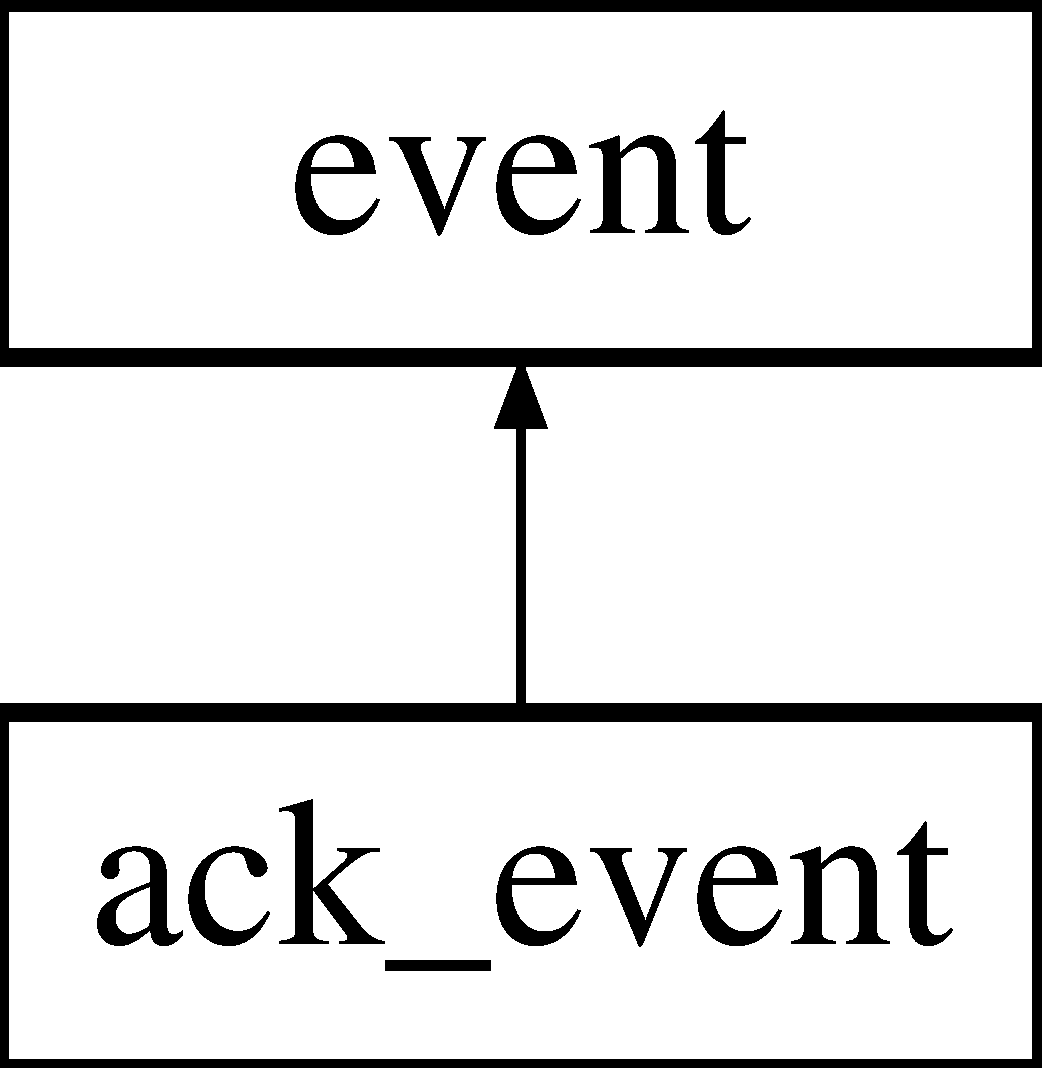
\includegraphics[height=2.000000cm]{classack__event}
\end{center}
\end{figure}
\subsection*{Public Member Functions}
\begin{DoxyCompactItemize}
\item 
\hyperlink{classack__event_ad3ac242accdc6db4f37da57a28e7f120}{ack\-\_\-event} ()
\begin{DoxyCompactList}\small\item\em Default constructor, sets everything to dummy or N\-U\-L\-L. \end{DoxyCompactList}\item 
\hypertarget{classack__event_a5a1e4cc597de2f0fda0a454a47544ef6}{\hyperlink{classack__event_a5a1e4cc597de2f0fda0a454a47544ef6}{ack\-\_\-event} (double time, \hyperlink{classsimulation}{simulation} \&\hyperlink{classevent_a08c6d828bfb6f5539dcd1491e8ac77d2}{sim}, \hyperlink{classnetflow}{netflow} \&flow, \hyperlink{classpacket}{packet} \&dup\-\_\-pkt)}\label{classack__event_a5a1e4cc597de2f0fda0a454a47544ef6}

\begin{DoxyCompactList}\small\item\em Initializes this event's time to the given one, sets the event I\-D, and sets the flow to which this \hyperlink{classack__event}{ack\-\_\-event} belongs. \end{DoxyCompactList}\item 
\hyperlink{classack__event_aa5e993d447f4d3bccc2559af3526a138}{$\sim$ack\-\_\-event} ()
\begin{DoxyCompactList}\small\item\em Destructor. \end{DoxyCompactList}\item 
\hypertarget{classack__event_a7c56c7da987f6092c855d27a114e9b33}{void \hyperlink{classack__event_a7c56c7da987f6092c855d27a114e9b33}{run\-Event} ()}\label{classack__event_a7c56c7da987f6092c855d27a114e9b33}

\begin{DoxyCompactList}\small\item\em Send an A\-C\-K packet then chains (queues another) \hyperlink{classack__event}{ack\-\_\-event}. \end{DoxyCompactList}\item 
void \hyperlink{classack__event_a56be0eef82f482ebb0d63277ae9429de}{print\-Helper} (ostream \&os)
\begin{DoxyCompactList}\small\item\em Print helper function. \end{DoxyCompactList}\end{DoxyCompactItemize}
\subsection*{Additional Inherited Members}


\subsection{Detailed Description}
This event should be queued when a destination host wants to send an A\-C\-K (not just duplicate A\-C\-Ks--any A\-C\-K\-S). 

The event automatically queues another \hyperlink{classack__event}{ack\-\_\-event} so that duplicate A\-C\-Ks will be sent in the future if the destination doesn't get the correct F\-L\-O\-W packets. Pending ack\-\_\-events should be cancelled when the destination gets the correct F\-L\-O\-W packet. 

\subsection{Constructor \& Destructor Documentation}
\hypertarget{classack__event_ad3ac242accdc6db4f37da57a28e7f120}{\index{ack\-\_\-event@{ack\-\_\-event}!ack\-\_\-event@{ack\-\_\-event}}
\index{ack\-\_\-event@{ack\-\_\-event}!ack_event@{ack\-\_\-event}}
\subsubsection[{ack\-\_\-event}]{\setlength{\rightskip}{0pt plus 5cm}ack\-\_\-event\-::ack\-\_\-event (
\begin{DoxyParamCaption}
{}
\end{DoxyParamCaption}
)}}\label{classack__event_ad3ac242accdc6db4f37da57a28e7f120}


Default constructor, sets everything to dummy or N\-U\-L\-L. 

\hypertarget{classack__event_aa5e993d447f4d3bccc2559af3526a138}{\index{ack\-\_\-event@{ack\-\_\-event}!$\sim$ack\-\_\-event@{$\sim$ack\-\_\-event}}
\index{$\sim$ack\-\_\-event@{$\sim$ack\-\_\-event}!ack_event@{ack\-\_\-event}}
\subsubsection[{$\sim$ack\-\_\-event}]{\setlength{\rightskip}{0pt plus 5cm}ack\-\_\-event\-::$\sim$ack\-\_\-event (
\begin{DoxyParamCaption}
{}
\end{DoxyParamCaption}
)}}\label{classack__event_aa5e993d447f4d3bccc2559af3526a138}


Destructor. 



\subsection{Member Function Documentation}
\hypertarget{classack__event_a56be0eef82f482ebb0d63277ae9429de}{\index{ack\-\_\-event@{ack\-\_\-event}!print\-Helper@{print\-Helper}}
\index{print\-Helper@{print\-Helper}!ack_event@{ack\-\_\-event}}
\subsubsection[{print\-Helper}]{\setlength{\rightskip}{0pt plus 5cm}void ack\-\_\-event\-::print\-Helper (
\begin{DoxyParamCaption}
\item[{ostream \&}]{os}
\end{DoxyParamCaption}
)\hspace{0.3cm}{\ttfamily [virtual]}}}\label{classack__event_a56be0eef82f482ebb0d63277ae9429de}


Print helper function. 


\begin{DoxyParams}{Parameters}
{\em os} & The output stream to which to write event information. \\
\hline
\end{DoxyParams}


Reimplemented from \hyperlink{classevent_a14ef1b59ef1f5a8311c7cac315c271df}{event}.



The documentation for this class was generated from the following files\-:\begin{DoxyCompactItemize}
\item 
src/\hyperlink{events_8h}{events.\-h}\item 
src/events.\-cpp\end{DoxyCompactItemize}

\hypertarget{classevent}{\section{event Class Reference}
\label{classevent}\index{event@{event}}
}


Base class for events in our event-\/driven network simulation.  




{\ttfamily \#include $<$events.\-h$>$}

Inheritance diagram for event\-:\begin{figure}[H]
\begin{center}
\leavevmode
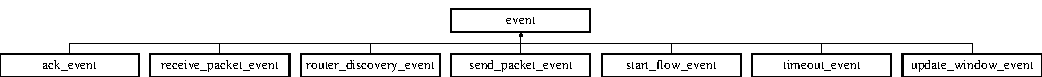
\includegraphics[height=1.032258cm]{classevent}
\end{center}
\end{figure}
\subsection*{Public Member Functions}
\begin{DoxyCompactItemize}
\item 
\hyperlink{classevent_a84a06dad1594d2d2a1d8bddff672d0a4}{event} ()
\begin{DoxyCompactList}\small\item\em Default constructor; sets time and I\-D to -\/1 and simulation to N\-U\-L\-L. \end{DoxyCompactList}\item 
\hyperlink{classevent_a10e6da45183cb40ae459dd2ab85e703d}{event} (double time, \hyperlink{classsimulation}{simulation} \&\hyperlink{classevent_a08c6d828bfb6f5539dcd1491e8ac77d2}{sim})
\begin{DoxyCompactList}\small\item\em Initializes this event's time to the given one and sets the event id to whatever the static I\-D generates spits out. \end{DoxyCompactList}\item 
\hypertarget{classevent_a9027354d797205dd1369b46f3485b8c4}{virtual \hyperlink{classevent_a9027354d797205dd1369b46f3485b8c4}{$\sim$event} ()}\label{classevent_a9027354d797205dd1369b46f3485b8c4}

\begin{DoxyCompactList}\small\item\em Destructor. \end{DoxyCompactList}\item 
double \hyperlink{classevent_a2ae66b1312a12b3b9f1bb7fa52bd8cc8}{get\-Time} () const 
\begin{DoxyCompactList}\small\item\em Getter for the time at which this event should run. \end{DoxyCompactList}\item 
long \hyperlink{classevent_ae287298290b26de20a09d6b63a201697}{get\-Id} () const 
\begin{DoxyCompactList}\small\item\em Getter for the unique I\-D number generated for this event. \end{DoxyCompactList}\item 
virtual void \hyperlink{classevent_a74b7b9e3b4dd30fb42a2612968def7ef}{run\-Event} ()
\begin{DoxyCompactList}\small\item\em Subclasses--i.\-e. \end{DoxyCompactList}\item 
virtual void \hyperlink{classevent_a14ef1b59ef1f5a8311c7cac315c271df}{print\-Helper} (ostream \&os)
\begin{DoxyCompactList}\small\item\em Print helper function. \end{DoxyCompactList}\end{DoxyCompactItemize}
\subsection*{Static Public Attributes}
\begin{DoxyCompactItemize}
\item 
static long \hyperlink{classevent_acdf8529e2178b7f7604beee6d8d459c3}{id\-\_\-generator} = 1
\begin{DoxyCompactList}\small\item\em Unique I\-D number generator. \end{DoxyCompactList}\end{DoxyCompactItemize}
\subsection*{Protected Attributes}
\begin{DoxyCompactItemize}
\item 
\hypertarget{classevent_a08c6d828bfb6f5539dcd1491e8ac77d2}{\hyperlink{classsimulation}{simulation} $\ast$ \hyperlink{classevent_a08c6d828bfb6f5539dcd1491e8ac77d2}{sim}}\label{classevent_a08c6d828bfb6f5539dcd1491e8ac77d2}

\begin{DoxyCompactList}\small\item\em Pointer to simulation this event is in so generated events can be added to its events queue. \end{DoxyCompactList}\end{DoxyCompactItemize}


\subsection{Detailed Description}
Base class for events in our event-\/driven network simulation. 

\subsection{Constructor \& Destructor Documentation}
\hypertarget{classevent_a84a06dad1594d2d2a1d8bddff672d0a4}{\index{event@{event}!event@{event}}
\index{event@{event}!event@{event}}
\subsubsection[{event}]{\setlength{\rightskip}{0pt plus 5cm}event\-::event (
\begin{DoxyParamCaption}
{}
\end{DoxyParamCaption}
)}}\label{classevent_a84a06dad1594d2d2a1d8bddff672d0a4}


Default constructor; sets time and I\-D to -\/1 and simulation to N\-U\-L\-L. 

\hypertarget{classevent_a10e6da45183cb40ae459dd2ab85e703d}{\index{event@{event}!event@{event}}
\index{event@{event}!event@{event}}
\subsubsection[{event}]{\setlength{\rightskip}{0pt plus 5cm}event\-::event (
\begin{DoxyParamCaption}
\item[{double}]{time, }
\item[{{\bf simulation} \&}]{sim}
\end{DoxyParamCaption}
)}}\label{classevent_a10e6da45183cb40ae459dd2ab85e703d}


Initializes this event's time to the given one and sets the event id to whatever the static I\-D generates spits out. 

Also sets the simulation pointer. 
\begin{DoxyParams}{Parameters}
{\em time} & at which this event should run \\
\hline
{\em sim} & \\
\hline
\end{DoxyParams}


\subsection{Member Function Documentation}
\hypertarget{classevent_ae287298290b26de20a09d6b63a201697}{\index{event@{event}!get\-Id@{get\-Id}}
\index{get\-Id@{get\-Id}!event@{event}}
\subsubsection[{get\-Id}]{\setlength{\rightskip}{0pt plus 5cm}long event\-::get\-Id (
\begin{DoxyParamCaption}
{}
\end{DoxyParamCaption}
) const}}\label{classevent_ae287298290b26de20a09d6b63a201697}


Getter for the unique I\-D number generated for this event. 

\begin{DoxyReturn}{Returns}
I\-D number 
\end{DoxyReturn}
\hypertarget{classevent_a2ae66b1312a12b3b9f1bb7fa52bd8cc8}{\index{event@{event}!get\-Time@{get\-Time}}
\index{get\-Time@{get\-Time}!event@{event}}
\subsubsection[{get\-Time}]{\setlength{\rightskip}{0pt plus 5cm}double event\-::get\-Time (
\begin{DoxyParamCaption}
{}
\end{DoxyParamCaption}
) const}}\label{classevent_a2ae66b1312a12b3b9f1bb7fa52bd8cc8}


Getter for the time at which this event should run. 

\begin{DoxyReturn}{Returns}
time at which this event should run. 
\end{DoxyReturn}
\hypertarget{classevent_a14ef1b59ef1f5a8311c7cac315c271df}{\index{event@{event}!print\-Helper@{print\-Helper}}
\index{print\-Helper@{print\-Helper}!event@{event}}
\subsubsection[{print\-Helper}]{\setlength{\rightskip}{0pt plus 5cm}void event\-::print\-Helper (
\begin{DoxyParamCaption}
\item[{ostream \&}]{os}
\end{DoxyParamCaption}
)\hspace{0.3cm}{\ttfamily [virtual]}}}\label{classevent_a14ef1b59ef1f5a8311c7cac315c271df}


Print helper function. 

Derived classes should (partially) override this. 
\begin{DoxyParams}{Parameters}
{\em os} & The output stream to which to write event information. \\
\hline
\end{DoxyParams}


Reimplemented in \hyperlink{classack__event_a56be0eef82f482ebb0d63277ae9429de}{ack\-\_\-event}, \hyperlink{classtimeout__event_a0c9c73de650b271dccfc6a7d3dedd3ec}{timeout\-\_\-event}, \hyperlink{classstart__flow__event_a75f4d4c3599f5ebc7813caccf07cde54}{start\-\_\-flow\-\_\-event}, \hyperlink{classsend__packet__event_a6f0f2911a15eef124ee57b1443a0b1d6}{send\-\_\-packet\-\_\-event}, \hyperlink{classupdate__window__event_ae533c05504abbf5dd9285a375c44e307}{update\-\_\-window\-\_\-event}, \hyperlink{classrouter__discovery__event_a32edb9914a54c925bbcb8a48d26451ed}{router\-\_\-discovery\-\_\-event}, and \hyperlink{classreceive__packet__event_a0da19ff9fc6f51c9599b095e064ee8ce}{receive\-\_\-packet\-\_\-event}.

\hypertarget{classevent_a74b7b9e3b4dd30fb42a2612968def7ef}{\index{event@{event}!run\-Event@{run\-Event}}
\index{run\-Event@{run\-Event}!event@{event}}
\subsubsection[{run\-Event}]{\setlength{\rightskip}{0pt plus 5cm}void event\-::run\-Event (
\begin{DoxyParamCaption}
{}
\end{DoxyParamCaption}
)\hspace{0.3cm}{\ttfamily [virtual]}}}\label{classevent_a74b7b9e3b4dd30fb42a2612968def7ef}


Subclasses--i.\-e. 

more specific events--will run operations like sending packets, adding new events to the simulation event queue, etc. Every event will log data. 

Reimplemented in \hyperlink{classack__event_a7c56c7da987f6092c855d27a114e9b33}{ack\-\_\-event}, \hyperlink{classtimeout__event_abacd620618ef70149548ca014fa7fd57}{timeout\-\_\-event}, \hyperlink{classstart__flow__event_a91f8f55565468bc294d89ccba846f759}{start\-\_\-flow\-\_\-event}, \hyperlink{classsend__packet__event_a844d3bf4a98011f4d128d05a8fb1a2db}{send\-\_\-packet\-\_\-event}, \hyperlink{classupdate__window__event_a41d9c1b343cd0ddceef94de6bc4abb68}{update\-\_\-window\-\_\-event}, \hyperlink{classrouter__discovery__event_a170768272244ac6578a7c38ffd82733f}{router\-\_\-discovery\-\_\-event}, and \hyperlink{classreceive__packet__event_ae7c0b0f1defa3e225373bea73f98b2ba}{receive\-\_\-packet\-\_\-event}.



\subsection{Member Data Documentation}
\hypertarget{classevent_acdf8529e2178b7f7604beee6d8d459c3}{\index{event@{event}!id\-\_\-generator@{id\-\_\-generator}}
\index{id\-\_\-generator@{id\-\_\-generator}!event@{event}}
\subsubsection[{id\-\_\-generator}]{\setlength{\rightskip}{0pt plus 5cm}long event\-::id\-\_\-generator = 1\hspace{0.3cm}{\ttfamily [static]}}}\label{classevent_acdf8529e2178b7f7604beee6d8d459c3}


Unique I\-D number generator. 

Initialized in corresponding cpp file. 

The documentation for this class was generated from the following files\-:\begin{DoxyCompactItemize}
\item 
src/\hyperlink{events_8h}{events.\-h}\item 
src/events.\-cpp\end{DoxyCompactItemize}

\hypertarget{classnetelement}{\section{netelement Class Reference}
\label{classnetelement}\index{netelement@{netelement}}
}


Superclass of all network elements including routers, hosts, links, packets, flows.  




{\ttfamily \#include $<$network.\-h$>$}

Inheritance diagram for netelement\-:\begin{figure}[H]
\begin{center}
\leavevmode
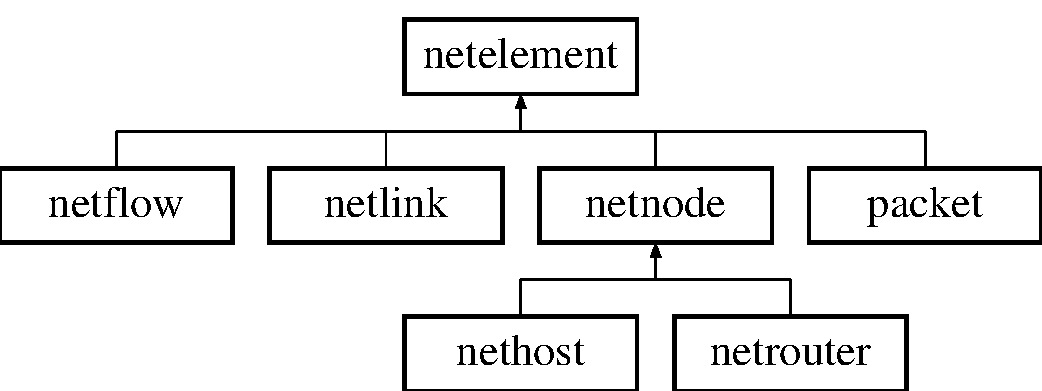
\includegraphics[height=3.000000cm]{classnetelement}
\end{center}
\end{figure}
\subsection*{Public Member Functions}
\begin{DoxyCompactItemize}
\item 
\hyperlink{classnetelement_a3c5679d2661bf66345db1e743bd3b134}{netelement} ()
\begin{DoxyCompactList}\small\item\em Default constructor. \end{DoxyCompactList}\item 
\hyperlink{classnetelement_a3bd01f2c0dba151f0f801ce3a9b64bd6}{netelement} (string name)
\begin{DoxyCompactList}\small\item\em Sets name to given one and sets nesting depth to 0. \end{DoxyCompactList}\item 
virtual \hyperlink{classnetelement_a5a19b5ac59274fe4e7da4588f9368f90}{$\sim$netelement} ()
\begin{DoxyCompactList}\small\item\em Destructor. \end{DoxyCompactList}\item 
const string \& \hyperlink{classnetelement_ae60065a5439cf34e8661a0f69e3a9b0e}{get\-Name} () const 
\begin{DoxyCompactList}\small\item\em Getter for name. \end{DoxyCompactList}\item 
void \hyperlink{classnetelement_a71b9122e5914b097d54453afd5f410dd}{set\-Nesting\-Depth} (int depth)
\begin{DoxyCompactList}\small\item\em Setter for the nesting depth. \end{DoxyCompactList}\item 
string \hyperlink{classnetelement_a6e5f6fd9636b94ecb10d9c60c3a52591}{nesting\-Prefix} (int delta) const 
\begin{DoxyCompactList}\small\item\em Gets a string with as many spaces as (nesting depth + delta) $\ast$ spaces per level. \end{DoxyCompactList}\item 
virtual void \hyperlink{classnetelement_a0763e38cebe07a50be6cfed014619de9}{print\-Helper} (std\-::ostream \&os) const 
\begin{DoxyCompactList}\small\item\em Print helper function. \end{DoxyCompactList}\end{DoxyCompactItemize}


\subsection{Detailed Description}
Superclass of all network elements including routers, hosts, links, packets, flows. 

\char`\"{}\-Device\char`\"{} is a bit of a misnomer for the latter but they all share a superclass so they can share an output operator overload and so they can co-\/exist in the same S\-T\-L collection if necessary. 

\subsection{Constructor \& Destructor Documentation}
\hypertarget{classnetelement_a3c5679d2661bf66345db1e743bd3b134}{\index{netelement@{netelement}!netelement@{netelement}}
\index{netelement@{netelement}!netelement@{netelement}}
\subsubsection[{netelement}]{\setlength{\rightskip}{0pt plus 5cm}netelement\-::netelement (
\begin{DoxyParamCaption}
{}
\end{DoxyParamCaption}
)}}\label{classnetelement_a3c5679d2661bf66345db1e743bd3b134}


Default constructor. 

Sets nesting depth to 0, name to empty string. \hypertarget{classnetelement_a3bd01f2c0dba151f0f801ce3a9b64bd6}{\index{netelement@{netelement}!netelement@{netelement}}
\index{netelement@{netelement}!netelement@{netelement}}
\subsubsection[{netelement}]{\setlength{\rightskip}{0pt plus 5cm}netelement\-::netelement (
\begin{DoxyParamCaption}
\item[{string}]{name}
\end{DoxyParamCaption}
)}}\label{classnetelement_a3bd01f2c0dba151f0f801ce3a9b64bd6}


Sets name to given one and sets nesting depth to 0. 


\begin{DoxyParams}{Parameters}
{\em name} & of this network element. \\
\hline
\end{DoxyParams}
\hypertarget{classnetelement_a5a19b5ac59274fe4e7da4588f9368f90}{\index{netelement@{netelement}!$\sim$netelement@{$\sim$netelement}}
\index{$\sim$netelement@{$\sim$netelement}!netelement@{netelement}}
\subsubsection[{$\sim$netelement}]{\setlength{\rightskip}{0pt plus 5cm}netelement\-::$\sim$netelement (
\begin{DoxyParamCaption}
{}
\end{DoxyParamCaption}
)\hspace{0.3cm}{\ttfamily [virtual]}}}\label{classnetelement_a5a19b5ac59274fe4e7da4588f9368f90}


Destructor. 



\subsection{Member Function Documentation}
\hypertarget{classnetelement_ae60065a5439cf34e8661a0f69e3a9b0e}{\index{netelement@{netelement}!get\-Name@{get\-Name}}
\index{get\-Name@{get\-Name}!netelement@{netelement}}
\subsubsection[{get\-Name}]{\setlength{\rightskip}{0pt plus 5cm}const string \& netelement\-::get\-Name (
\begin{DoxyParamCaption}
{}
\end{DoxyParamCaption}
) const}}\label{classnetelement_ae60065a5439cf34e8661a0f69e3a9b0e}


Getter for name. 

\begin{DoxyReturn}{Returns}
name of this network element. 
\end{DoxyReturn}
\hypertarget{classnetelement_a6e5f6fd9636b94ecb10d9c60c3a52591}{\index{netelement@{netelement}!nesting\-Prefix@{nesting\-Prefix}}
\index{nesting\-Prefix@{nesting\-Prefix}!netelement@{netelement}}
\subsubsection[{nesting\-Prefix}]{\setlength{\rightskip}{0pt plus 5cm}string netelement\-::nesting\-Prefix (
\begin{DoxyParamCaption}
\item[{int}]{delta}
\end{DoxyParamCaption}
) const}}\label{classnetelement_a6e5f6fd9636b94ecb10d9c60c3a52591}


Gets a string with as many spaces as (nesting depth + delta) $\ast$ spaces per level. 


\begin{DoxyParams}{Parameters}
{\em delta} & effective nesting depth will be actual depth + delta \\
\hline
\end{DoxyParams}
\begin{DoxyReturn}{Returns}
string with number of spaces determined by desting depth and the delta from that desting depth. 
\end{DoxyReturn}
\hypertarget{classnetelement_a0763e38cebe07a50be6cfed014619de9}{\index{netelement@{netelement}!print\-Helper@{print\-Helper}}
\index{print\-Helper@{print\-Helper}!netelement@{netelement}}
\subsubsection[{print\-Helper}]{\setlength{\rightskip}{0pt plus 5cm}void netelement\-::print\-Helper (
\begin{DoxyParamCaption}
\item[{std\-::ostream \&}]{os}
\end{DoxyParamCaption}
) const\hspace{0.3cm}{\ttfamily [virtual]}}}\label{classnetelement_a0763e38cebe07a50be6cfed014619de9}


Print helper function. 

Derived classes should (partially) override this. 
\begin{DoxyParams}{Parameters}
{\em os} & The output stream to which to write netdevice information. \\
\hline
\end{DoxyParams}


Reimplemented in \hyperlink{classnetnode_acf1330a7d57a1358064b3736b888b464}{netnode}.

\hypertarget{classnetelement_a71b9122e5914b097d54453afd5f410dd}{\index{netelement@{netelement}!set\-Nesting\-Depth@{set\-Nesting\-Depth}}
\index{set\-Nesting\-Depth@{set\-Nesting\-Depth}!netelement@{netelement}}
\subsubsection[{set\-Nesting\-Depth}]{\setlength{\rightskip}{0pt plus 5cm}void netelement\-::set\-Nesting\-Depth (
\begin{DoxyParamCaption}
\item[{int}]{depth}
\end{DoxyParamCaption}
)}}\label{classnetelement_a71b9122e5914b097d54453afd5f410dd}


Setter for the nesting depth. 


\begin{DoxyParams}{Parameters}
{\em depth} & \\
\hline
\end{DoxyParams}


The documentation for this class was generated from the following files\-:\begin{DoxyCompactItemize}
\item 
src/\hyperlink{network_8h}{network.\-h}\item 
src/network.\-cpp\end{DoxyCompactItemize}

\hypertarget{classnetflow}{\section{netflow Class Reference}
\label{classnetflow}\index{netflow@{netflow}}
}


Represents a flow in a simple network.  




{\ttfamily \#include $<$network.\-h$>$}

Inheritance diagram for netflow\-:\begin{figure}[H]
\begin{center}
\leavevmode
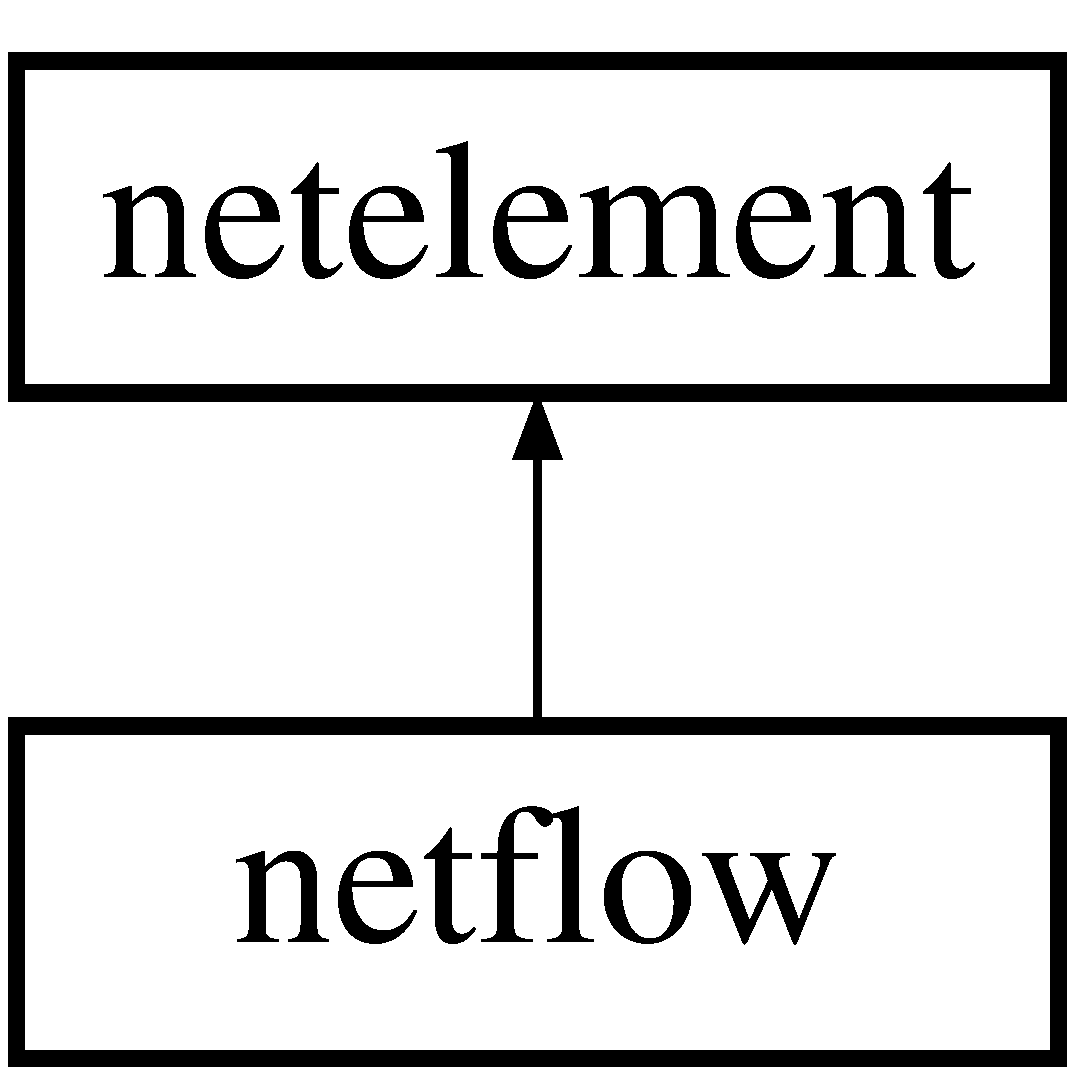
\includegraphics[height=2.000000cm]{classnetflow}
\end{center}
\end{figure}
\subsection*{Public Member Functions}
\begin{DoxyCompactItemize}
\item 
\hyperlink{classnetflow_aefd21ce2f7c362163e51776672e1ebeb}{netflow} (string name, double start\-\_\-time, double size\-\_\-mb, \hyperlink{classnethost}{nethost} \&source, \hyperlink{classnethost}{nethost} \&destination, bool using\-F\-A\-S\-T, \hyperlink{classsimulation}{simulation} \&sim)
\begin{DoxyCompactList}\small\item\em Initializes the flow's basic attributes as well as attributes required to perform T\-C\-P Reno transmissions, like window size, last A\-C\-K seen, number of duplicate A\-C\-Ks, etc. \end{DoxyCompactList}\item 
\hyperlink{classnetflow_ac64edff00ca0ff62217243ce8abb94e6}{netflow} (string name, double start\-\_\-time, double size\-\_\-mb, \hyperlink{classnethost}{nethost} \&source, \hyperlink{classnethost}{nethost} \&destination, \hyperlink{classsimulation}{simulation} \&sim)
\begin{DoxyCompactList}\small\item\em Same as other constructor but {\ttfamily using\-F\-A\-S\-T} is set to false. \end{DoxyCompactList}\item 
double \hyperlink{classnetflow_a6c89dfa31291104fd5207f10a4bb424b}{get\-Start\-Time\-Sec} () const 
\begin{DoxyCompactList}\small\item\em Getter for start time in seconds. \end{DoxyCompactList}\item 
double \hyperlink{classnetflow_a4ca3539d49814e6ffaf46c9db28d4cb1}{get\-Start\-Time\-Ms} () const 
\begin{DoxyCompactList}\small\item\em Getter for start time in milliseconds. \end{DoxyCompactList}\item 
double \hyperlink{classnetflow_a8afb866e40738f7038d18bdb9a572500}{get\-Size\-Mb} () const 
\begin{DoxyCompactList}\small\item\em Getter for size in megabits. \end{DoxyCompactList}\item 
\hyperlink{classnethost}{nethost} $\ast$ \hyperlink{classnetflow_a07af3290478934720fd1500f89c5586d}{get\-Destination} () const 
\begin{DoxyCompactList}\small\item\em Getter for pointer to destination host. \end{DoxyCompactList}\item 
\hyperlink{classnethost}{nethost} $\ast$ \hyperlink{classnetflow_a8a2f81127fcecaafeb83570dfb77d669}{get\-Source} () const 
\begin{DoxyCompactList}\small\item\em Getter for pointer to source host. \end{DoxyCompactList}\item 
int \hyperlink{classnetflow_a248e9f4bf73f873608bed283a7897340}{get\-Pkt\-Tally} () const 
\begin{DoxyCompactList}\small\item\em Getter for the count of flow packets received by destination within the interval. \end{DoxyCompactList}\item 
double \hyperlink{classnetflow_a21b2e6d775c5d8eab0adff3f238a41fc}{get\-Left\-Time} () const 
\begin{DoxyCompactList}\small\item\em Getter for the start time of the packet count interval. \end{DoxyCompactList}\item 
double \hyperlink{classnetflow_ad70e1973aa9856ec2eea2f54c578acc4}{get\-Right\-Time} () const 
\begin{DoxyCompactList}\small\item\em Getter for the ending time of the packet count interval. \end{DoxyCompactList}\item 
int \hyperlink{classnetflow_afd6c72736a88766d407f3a66871996bb}{get\-Num\-Total\-Packets} () const 
\begin{DoxyCompactList}\small\item\em Getter for number of packets used in a flawless transmission of this flow. \end{DoxyCompactList}\item 
double \hyperlink{classnetflow_a02e309d963c2bca12b77b66b890b9c66}{get\-Timeout\-Length\-Ms} () const 
\begin{DoxyCompactList}\small\item\em Getter for the dynamically adjusted timeout length in milliseconds. \end{DoxyCompactList}\item 
int \hyperlink{classnetflow_ac27a75c664720d1da286ec61906564db}{get\-Highest\-Ack\-Seqnum} () const 
\begin{DoxyCompactList}\small\item\em Getter for the sequence number of the last A\-C\-K seen. \end{DoxyCompactList}\item 
int \hyperlink{classnetflow_abee82205b8482a99036148d7ef869ae2}{get\-Num\-Duplicate\-Acks} () const 
\begin{DoxyCompactList}\small\item\em Getter for the number of duplicate A\-C\-Ks seen so far. \end{DoxyCompactList}\item 
double \hyperlink{classnetflow_a4825a3c57231c9f474e9cd1a76e60f66}{get\-Avg\-R\-T\-T} () const 
\begin{DoxyCompactList}\small\item\em Getter for the average round trip time. \end{DoxyCompactList}\item 
double \hyperlink{classnetflow_a58b013589d73c37349547c37a35db128}{get\-Min\-R\-T\-T} () const 
\begin{DoxyCompactList}\small\item\em Getter for the minimum round trip time seen so far for this flow. \end{DoxyCompactList}\item 
bool \hyperlink{classnetflow_ababb5a520cb2b826ad906bd9cade0ecb}{is\-Using\-F\-A\-S\-T} () const 
\begin{DoxyCompactList}\small\item\em True if using T\-C\-P F\-A\-S\-T, false if Tahoe. \end{DoxyCompactList}\item 
const map$<$ int, double $>$ \& \hyperlink{classnetflow_a08f6d8d01f51c861a00710a533f3b604}{get\-Round\-Trip\-Times} () const 
\begin{DoxyCompactList}\small\item\em Getter for a const reference to the round-\/trip times map. \end{DoxyCompactList}\item 
double \hyperlink{classnetflow_aa73fac7bfc0f25946e7b345f46115dc9}{get\-Window\-Size} () const 
\begin{DoxyCompactList}\small\item\em Getter for the current window size. \end{DoxyCompactList}\item 
int \hyperlink{classnetflow_a7c44701ace1f15dbef9227fb06f419af}{get\-Window\-Start} () const 
\begin{DoxyCompactList}\small\item\em Getter for the sequence number at which the current window starts. \end{DoxyCompactList}\item 
double \hyperlink{classnetflow_a7b2904e3229ddb7baba23c1c2abd4941}{get\-Lin\-Growth\-Winsize\-Threshold} () const 
\begin{DoxyCompactList}\small\item\em Getter for the linear growth threshold (i.\-e., the window size after which the window size will be increased as 1/n instead of 1 per A\-C\-K) \end{DoxyCompactList}\item 
virtual void \hyperlink{classnetflow_acbcb512e7ba8fb2f4dfb5c49f792b837}{print\-Helper} (ostream \&os) const 
\begin{DoxyCompactList}\small\item\em Print helper function which partially overrides the one in netdevice. \end{DoxyCompactList}\item 
double \hyperlink{classnetflow_a2f30ed4c8b1934dc70cad568b009384b}{get\-Flow\-Rate\-Bytes\-Per\-Sec} () const 
\begin{DoxyCompactList}\small\item\em Getter for the flow rate in bytes per second. \end{DoxyCompactList}\item 
double \hyperlink{classnetflow_a8e05bddc18878c14b815dba199996aa0}{get\-Flow\-Rate\-Mbps} (double time) const 
\begin{DoxyCompactList}\small\item\em Getter for the flow rate in megabits per second. \end{DoxyCompactList}\item 
double \hyperlink{classnetflow_ade54f5be8b44ca85de0f1b453857519d}{get\-Flow\-Percentage} () const 
\begin{DoxyCompactList}\small\item\em Getter for the percentage of flow that has been transmitted so far Useful for debugging; can be graphed along with other flow metrics. \end{DoxyCompactList}\item 
double \hyperlink{classnetflow_af9eaf8bcc1f369201b400ca8ffa98f34}{get\-Pkt\-Delay} (double curr\-Time) const 
\begin{DoxyCompactList}\small\item\em Packet delay is defined as time elapsed since packet is send and acknowledgment is received. \end{DoxyCompactList}\item 
void \hyperlink{classnetflow_afb017e85595e2d18ed839c26c5a37289}{set\-Source} (\hyperlink{classnethost}{nethost} \&source)
\begin{DoxyCompactList}\small\item\em Setter for the source host. \end{DoxyCompactList}\item 
void \hyperlink{classnetflow_a5ce0bbc79c6400fe89da80487f509415}{set\-Destination} (\hyperlink{classnethost}{nethost} \&destination)
\begin{DoxyCompactList}\small\item\em Setter for the destination host. \end{DoxyCompactList}\item 
void \hyperlink{classnetflow_a1b5aadc26000de914d77a0f18c3af2a9}{update\-Pkt\-Tally} (double time)
\begin{DoxyCompactList}\small\item\em Updates packet tally depending on whether {\ttfamily \hyperlink{classreceive__packet__event}{receive\-\_\-packet\-\_\-event}} occurs during rate\-\_\-interval. \end{DoxyCompactList}\item 
void \hyperlink{classnetflow_a9f3ef1670c996d54dbd32a1c941e2d83}{set\-F\-A\-S\-T\-Window\-Size} (double new\-\_\-size)
\begin{DoxyCompactList}\small\item\em Changes a flow's window size during an \hyperlink{classupdate__window__event}{update\-\_\-window\-\_\-event}. \end{DoxyCompactList}\item 
void \hyperlink{classnetflow_ad91146f3b19e8d2812e297714a4ef5d4}{set\-Left\-Time} (double new\-Time)
\begin{DoxyCompactList}\small\item\em Sets left time. \end{DoxyCompactList}\item 
void \hyperlink{classnetflow_a09b799f9166e0df50091a73516063c64}{set\-Right\-Time} (double new\-Time)
\begin{DoxyCompactList}\small\item\em Sets right time. \end{DoxyCompactList}\item 
void \hyperlink{classnetflow_a5865695e5360027ce36e047b3368ff25}{register\-Ack\-Event} (int seq, double time)
\begin{DoxyCompactList}\small\item\em Makes an {\ttfamily \hyperlink{classack__event}{ack\-\_\-event}} and puts it on the simulation's event queue. \end{DoxyCompactList}\item 
vector$<$ \hyperlink{classpacket}{packet} $>$ \hyperlink{classnetflow_ad9974ffa5f9b264b561355c07bc0bd9f}{peek\-Outstanding\-Packets} ()
\begin{DoxyCompactList}\small\item\em Gets all the packets in this window that must be sent. \end{DoxyCompactList}\item 
vector$<$ \hyperlink{classpacket}{packet} $>$ \hyperlink{classnetflow_ae072b9c8069401bbc45e6ad9853eb45f}{pop\-Outstanding\-Packets} (double start\-\_\-time, double link\-Free\-At)
\begin{DoxyCompactList}\small\item\em Gets all the packets in this window that must be sent. \end{DoxyCompactList}\item 
void \hyperlink{classnetflow_a7d2582540a1cc34a7fc5b1c6ce41d329}{received\-Ack} (\hyperlink{classpacket}{packet} \&pkt, double end\-\_\-time\-\_\-ms, double link\-Free\-At\-Time)
\begin{DoxyCompactList}\small\item\em When an A\-C\-K is received (it's assumed that the packet is arriving at this flow's source) this function must be called so the window will slide and resize, so duplicate A\-C\-Ks will register, and so the timeout length will adjust. \end{DoxyCompactList}\item 
void \hyperlink{classnetflow_a3fab65a6f9fbfe3f54af066d260cd0b8}{received\-Flow\-Packet} (\hyperlink{classpacket}{packet} \&pkt, double arrival\-\_\-time)
\begin{DoxyCompactList}\small\item\em When a F\-L\-O\-W packet is received (it's assumed that the packet is arriving at this flow's destination) this function should be called to make and queue an immediate duplicate\-\_\-ack\-\_\-event. \end{DoxyCompactList}\item 
void \hyperlink{classnetflow_ad914b2fc48fd4727464619823b09a856}{timeout\-Occurred} ()
\begin{DoxyCompactList}\small\item\em This function should be called after a timeout so the window size can change accordingly and so the old \hyperlink{classtimeout__event}{timeout\-\_\-event} can be cancelled. \end{DoxyCompactList}\end{DoxyCompactItemize}
\subsection*{Static Public Attributes}
\begin{DoxyCompactItemize}
\item 
static const int \hyperlink{classnetflow_ace7122626410ab50fbe69dcc0f77dcb0}{F\-A\-S\-T\-\_\-\-R\-E\-T\-R\-A\-N\-S\-M\-I\-T\-\_\-\-D\-U\-P\-L\-I\-C\-A\-T\-E\-\_\-\-A\-C\-K\-\_\-\-T\-H\-R\-E\-S\-H\-O\-L\-D} = 3
\begin{DoxyCompactList}\small\item\em Number of duplicate A\-C\-Ks before fast retransmit is used. \end{DoxyCompactList}\item 
\hypertarget{classnetflow_a7dd619873b5d292074adc5d4ec0aa103}{static constexpr double \hyperlink{classnetflow_a7dd619873b5d292074adc5d4ec0aa103}{D\-E\-F\-A\-U\-L\-T\-\_\-\-I\-N\-I\-T\-I\-A\-L\-\_\-\-T\-I\-M\-E\-O\-U\-T} = 1000.\-0}\label{classnetflow_a7dd619873b5d292074adc5d4ec0aa103}

\begin{DoxyCompactList}\small\item\em The timeout value for the very first packet sent in a flow; the timeout value is later seeded with the first packet's R\-T\-T and then changed with recursive average and deviation algorithms. \end{DoxyCompactList}\item 
static constexpr double \hyperlink{classnetflow_a0461fac67c5f304973461a1644b58dd3}{B\-\_\-\-T\-I\-M\-E\-O\-U\-T\-\_\-\-C\-A\-L\-C} = 0.\-1
\begin{DoxyCompactList}\small\item\em The constant 'b' from the recursive average and std formulas. \end{DoxyCompactList}\item 
\hypertarget{classnetflow_abfab6219768889c4b22a382d3be2147d}{static constexpr double \hyperlink{classnetflow_abfab6219768889c4b22a382d3be2147d}{T\-I\-M\-E\-\_\-\-E\-P\-S\-I\-L\-O\-N} = 0.\-0000000001}\label{classnetflow_abfab6219768889c4b22a382d3be2147d}

\begin{DoxyCompactList}\small\item\em A small fraction of a millisecond used to order timeout events and regular send packet events. \end{DoxyCompactList}\end{DoxyCompactItemize}


\subsection{Detailed Description}
Represents a flow in a simple network. 

Uses various constants defined in {\ttfamily util.\-cpp}. 

\subsection{Constructor \& Destructor Documentation}
\hypertarget{classnetflow_aefd21ce2f7c362163e51776672e1ebeb}{\index{netflow@{netflow}!netflow@{netflow}}
\index{netflow@{netflow}!netflow@{netflow}}
\subsubsection[{netflow}]{\setlength{\rightskip}{0pt plus 5cm}netflow\-::netflow (
\begin{DoxyParamCaption}
\item[{string}]{name, }
\item[{double}]{start\-\_\-time, }
\item[{double}]{size\-\_\-mb, }
\item[{{\bf nethost} \&}]{source, }
\item[{{\bf nethost} \&}]{destination, }
\item[{bool}]{using\-F\-A\-S\-T, }
\item[{{\bf simulation} \&}]{sim}
\end{DoxyParamCaption}
)}}\label{classnetflow_aefd21ce2f7c362163e51776672e1ebeb}


Initializes the flow's basic attributes as well as attributes required to perform T\-C\-P Reno transmissions, like window size, last A\-C\-K seen, number of duplicate A\-C\-Ks, etc. 


\begin{DoxyParams}{Parameters}
{\em name} & of this flow \\
\hline
{\em start\-\_\-time} & in seconds at which this flow starts \\
\hline
{\em size\-\_\-mb} & size of this flow in megabits \\
\hline
{\em source} & host at which this flow starts \\
\hline
{\em destination} & host at which this flow ends \\
\hline
{\em using\-F\-A\-S\-T} & true if using F\-A\-S\-T T\-C\-P, false if using T\-C\-P Tahoe \\
\hline
{\em sim} & \\
\hline
\end{DoxyParams}
\hypertarget{classnetflow_ac64edff00ca0ff62217243ce8abb94e6}{\index{netflow@{netflow}!netflow@{netflow}}
\index{netflow@{netflow}!netflow@{netflow}}
\subsubsection[{netflow}]{\setlength{\rightskip}{0pt plus 5cm}netflow\-::netflow (
\begin{DoxyParamCaption}
\item[{string}]{name, }
\item[{double}]{start\-\_\-time, }
\item[{double}]{size\-\_\-mb, }
\item[{{\bf nethost} \&}]{source, }
\item[{{\bf nethost} \&}]{destination, }
\item[{{\bf simulation} \&}]{sim}
\end{DoxyParamCaption}
)}}\label{classnetflow_ac64edff00ca0ff62217243ce8abb94e6}


Same as other constructor but {\ttfamily using\-F\-A\-S\-T} is set to false. 


\begin{DoxyParams}{Parameters}
{\em name} & of this flow \\
\hline
{\em start\-\_\-time} & in seconds at which this flow starts \\
\hline
{\em size\-\_\-mb} & size of this flow in megabits \\
\hline
{\em source} & host at which this flow starts \\
\hline
{\em destination} & host at which this flow ends \\
\hline
{\em sim} & \\
\hline
\end{DoxyParams}


\subsection{Member Function Documentation}
\hypertarget{classnetflow_a4825a3c57231c9f474e9cd1a76e60f66}{\index{netflow@{netflow}!get\-Avg\-R\-T\-T@{get\-Avg\-R\-T\-T}}
\index{get\-Avg\-R\-T\-T@{get\-Avg\-R\-T\-T}!netflow@{netflow}}
\subsubsection[{get\-Avg\-R\-T\-T}]{\setlength{\rightskip}{0pt plus 5cm}double netflow\-::get\-Avg\-R\-T\-T (
\begin{DoxyParamCaption}
{}
\end{DoxyParamCaption}
) const}}\label{classnetflow_a4825a3c57231c9f474e9cd1a76e60f66}


Getter for the average round trip time. 

\begin{DoxyReturn}{Returns}
average R\-T\-T 
\end{DoxyReturn}
\hypertarget{classnetflow_a07af3290478934720fd1500f89c5586d}{\index{netflow@{netflow}!get\-Destination@{get\-Destination}}
\index{get\-Destination@{get\-Destination}!netflow@{netflow}}
\subsubsection[{get\-Destination}]{\setlength{\rightskip}{0pt plus 5cm}{\bf nethost} $\ast$ netflow\-::get\-Destination (
\begin{DoxyParamCaption}
{}
\end{DoxyParamCaption}
) const}}\label{classnetflow_a07af3290478934720fd1500f89c5586d}


Getter for pointer to destination host. 

\begin{DoxyReturn}{Returns}
pointer to destination host. 
\end{DoxyReturn}
\hypertarget{classnetflow_ade54f5be8b44ca85de0f1b453857519d}{\index{netflow@{netflow}!get\-Flow\-Percentage@{get\-Flow\-Percentage}}
\index{get\-Flow\-Percentage@{get\-Flow\-Percentage}!netflow@{netflow}}
\subsubsection[{get\-Flow\-Percentage}]{\setlength{\rightskip}{0pt plus 5cm}double netflow\-::get\-Flow\-Percentage (
\begin{DoxyParamCaption}
{}
\end{DoxyParamCaption}
) const}}\label{classnetflow_ade54f5be8b44ca85de0f1b453857519d}


Getter for the percentage of flow that has been transmitted so far Useful for debugging; can be graphed along with other flow metrics. 

\begin{DoxyReturn}{Returns}
the percentage of the flow that's been completed. 
\end{DoxyReturn}
\hypertarget{classnetflow_a2f30ed4c8b1934dc70cad568b009384b}{\index{netflow@{netflow}!get\-Flow\-Rate\-Bytes\-Per\-Sec@{get\-Flow\-Rate\-Bytes\-Per\-Sec}}
\index{get\-Flow\-Rate\-Bytes\-Per\-Sec@{get\-Flow\-Rate\-Bytes\-Per\-Sec}!netflow@{netflow}}
\subsubsection[{get\-Flow\-Rate\-Bytes\-Per\-Sec}]{\setlength{\rightskip}{0pt plus 5cm}double netflow\-::get\-Flow\-Rate\-Bytes\-Per\-Sec (
\begin{DoxyParamCaption}
{}
\end{DoxyParamCaption}
) const}}\label{classnetflow_a2f30ed4c8b1934dc70cad568b009384b}


Getter for the flow rate in bytes per second. 

\begin{DoxyReturn}{Returns}
flow rate in bytes/sec. 
\end{DoxyReturn}
\hypertarget{classnetflow_a8e05bddc18878c14b815dba199996aa0}{\index{netflow@{netflow}!get\-Flow\-Rate\-Mbps@{get\-Flow\-Rate\-Mbps}}
\index{get\-Flow\-Rate\-Mbps@{get\-Flow\-Rate\-Mbps}!netflow@{netflow}}
\subsubsection[{get\-Flow\-Rate\-Mbps}]{\setlength{\rightskip}{0pt plus 5cm}double netflow\-::get\-Flow\-Rate\-Mbps (
\begin{DoxyParamCaption}
\item[{double}]{time}
\end{DoxyParamCaption}
) const}}\label{classnetflow_a8e05bddc18878c14b815dba199996aa0}


Getter for the flow rate in megabits per second. 

\begin{DoxyReturn}{Returns}
flow rate. 
\end{DoxyReturn}
\hypertarget{classnetflow_ac27a75c664720d1da286ec61906564db}{\index{netflow@{netflow}!get\-Highest\-Ack\-Seqnum@{get\-Highest\-Ack\-Seqnum}}
\index{get\-Highest\-Ack\-Seqnum@{get\-Highest\-Ack\-Seqnum}!netflow@{netflow}}
\subsubsection[{get\-Highest\-Ack\-Seqnum}]{\setlength{\rightskip}{0pt plus 5cm}int netflow\-::get\-Highest\-Ack\-Seqnum (
\begin{DoxyParamCaption}
{}
\end{DoxyParamCaption}
) const}}\label{classnetflow_ac27a75c664720d1da286ec61906564db}


Getter for the sequence number of the last A\-C\-K seen. 

\begin{DoxyReturn}{Returns}
last A\-C\-K's sequence number. 
\end{DoxyReturn}
\hypertarget{classnetflow_a21b2e6d775c5d8eab0adff3f238a41fc}{\index{netflow@{netflow}!get\-Left\-Time@{get\-Left\-Time}}
\index{get\-Left\-Time@{get\-Left\-Time}!netflow@{netflow}}
\subsubsection[{get\-Left\-Time}]{\setlength{\rightskip}{0pt plus 5cm}double netflow\-::get\-Left\-Time (
\begin{DoxyParamCaption}
{}
\end{DoxyParamCaption}
) const}}\label{classnetflow_a21b2e6d775c5d8eab0adff3f238a41fc}


Getter for the start time of the packet count interval. 

\begin{DoxyReturn}{Returns}
left side of pkt count interval 
\end{DoxyReturn}
\hypertarget{classnetflow_a7b2904e3229ddb7baba23c1c2abd4941}{\index{netflow@{netflow}!get\-Lin\-Growth\-Winsize\-Threshold@{get\-Lin\-Growth\-Winsize\-Threshold}}
\index{get\-Lin\-Growth\-Winsize\-Threshold@{get\-Lin\-Growth\-Winsize\-Threshold}!netflow@{netflow}}
\subsubsection[{get\-Lin\-Growth\-Winsize\-Threshold}]{\setlength{\rightskip}{0pt plus 5cm}double netflow\-::get\-Lin\-Growth\-Winsize\-Threshold (
\begin{DoxyParamCaption}
{}
\end{DoxyParamCaption}
) const}}\label{classnetflow_a7b2904e3229ddb7baba23c1c2abd4941}


Getter for the linear growth threshold (i.\-e., the window size after which the window size will be increased as 1/n instead of 1 per A\-C\-K) 

\begin{DoxyReturn}{Returns}
linear growth window size threshold 
\end{DoxyReturn}
\hypertarget{classnetflow_a58b013589d73c37349547c37a35db128}{\index{netflow@{netflow}!get\-Min\-R\-T\-T@{get\-Min\-R\-T\-T}}
\index{get\-Min\-R\-T\-T@{get\-Min\-R\-T\-T}!netflow@{netflow}}
\subsubsection[{get\-Min\-R\-T\-T}]{\setlength{\rightskip}{0pt plus 5cm}double netflow\-::get\-Min\-R\-T\-T (
\begin{DoxyParamCaption}
{}
\end{DoxyParamCaption}
) const}}\label{classnetflow_a58b013589d73c37349547c37a35db128}


Getter for the minimum round trip time seen so far for this flow. 

\begin{DoxyReturn}{Returns}
min R\-T\-T 
\end{DoxyReturn}
\hypertarget{classnetflow_abee82205b8482a99036148d7ef869ae2}{\index{netflow@{netflow}!get\-Num\-Duplicate\-Acks@{get\-Num\-Duplicate\-Acks}}
\index{get\-Num\-Duplicate\-Acks@{get\-Num\-Duplicate\-Acks}!netflow@{netflow}}
\subsubsection[{get\-Num\-Duplicate\-Acks}]{\setlength{\rightskip}{0pt plus 5cm}int netflow\-::get\-Num\-Duplicate\-Acks (
\begin{DoxyParamCaption}
{}
\end{DoxyParamCaption}
) const}}\label{classnetflow_abee82205b8482a99036148d7ef869ae2}


Getter for the number of duplicate A\-C\-Ks seen so far. 

\begin{DoxyReturn}{Returns}
num duplicate A\-C\-Ks 
\end{DoxyReturn}
\hypertarget{classnetflow_afd6c72736a88766d407f3a66871996bb}{\index{netflow@{netflow}!get\-Num\-Total\-Packets@{get\-Num\-Total\-Packets}}
\index{get\-Num\-Total\-Packets@{get\-Num\-Total\-Packets}!netflow@{netflow}}
\subsubsection[{get\-Num\-Total\-Packets}]{\setlength{\rightskip}{0pt plus 5cm}int netflow\-::get\-Num\-Total\-Packets (
\begin{DoxyParamCaption}
{}
\end{DoxyParamCaption}
) const}}\label{classnetflow_afd6c72736a88766d407f3a66871996bb}


Getter for number of packets used in a flawless transmission of this flow. 

In reality some packets may be dropped or lost, so this is really the largest packet sequence number in this flow, where the first packet has a sequence number of 1. \begin{DoxyReturn}{Returns}
number of packets in this flow 
\end{DoxyReturn}
\hypertarget{classnetflow_af9eaf8bcc1f369201b400ca8ffa98f34}{\index{netflow@{netflow}!get\-Pkt\-Delay@{get\-Pkt\-Delay}}
\index{get\-Pkt\-Delay@{get\-Pkt\-Delay}!netflow@{netflow}}
\subsubsection[{get\-Pkt\-Delay}]{\setlength{\rightskip}{0pt plus 5cm}double netflow\-::get\-Pkt\-Delay (
\begin{DoxyParamCaption}
\item[{double}]{curr\-Time}
\end{DoxyParamCaption}
) const}}\label{classnetflow_af9eaf8bcc1f369201b400ca8ffa98f34}


Packet delay is defined as time elapsed since packet is send and acknowledgment is received. 


\begin{DoxyParams}{Parameters}
{\em curr\-Time} & current time \\
\hline
\end{DoxyParams}
\begin{DoxyReturn}{Returns}
packet delay 
\end{DoxyReturn}
\hypertarget{classnetflow_a248e9f4bf73f873608bed283a7897340}{\index{netflow@{netflow}!get\-Pkt\-Tally@{get\-Pkt\-Tally}}
\index{get\-Pkt\-Tally@{get\-Pkt\-Tally}!netflow@{netflow}}
\subsubsection[{get\-Pkt\-Tally}]{\setlength{\rightskip}{0pt plus 5cm}int netflow\-::get\-Pkt\-Tally (
\begin{DoxyParamCaption}
{}
\end{DoxyParamCaption}
) const}}\label{classnetflow_a248e9f4bf73f873608bed283a7897340}


Getter for the count of flow packets received by destination within the interval. 

\begin{DoxyReturn}{Returns}
number of flow packets received 
\end{DoxyReturn}
\hypertarget{classnetflow_ad70e1973aa9856ec2eea2f54c578acc4}{\index{netflow@{netflow}!get\-Right\-Time@{get\-Right\-Time}}
\index{get\-Right\-Time@{get\-Right\-Time}!netflow@{netflow}}
\subsubsection[{get\-Right\-Time}]{\setlength{\rightskip}{0pt plus 5cm}double netflow\-::get\-Right\-Time (
\begin{DoxyParamCaption}
{}
\end{DoxyParamCaption}
) const}}\label{classnetflow_ad70e1973aa9856ec2eea2f54c578acc4}


Getter for the ending time of the packet count interval. 

\begin{DoxyReturn}{Returns}
right side of pkt count interval 
\end{DoxyReturn}
\hypertarget{classnetflow_a08f6d8d01f51c861a00710a533f3b604}{\index{netflow@{netflow}!get\-Round\-Trip\-Times@{get\-Round\-Trip\-Times}}
\index{get\-Round\-Trip\-Times@{get\-Round\-Trip\-Times}!netflow@{netflow}}
\subsubsection[{get\-Round\-Trip\-Times}]{\setlength{\rightskip}{0pt plus 5cm}const map$<$ int, double $>$ \& netflow\-::get\-Round\-Trip\-Times (
\begin{DoxyParamCaption}
{}
\end{DoxyParamCaption}
) const}}\label{classnetflow_a08f6d8d01f51c861a00710a533f3b604}


Getter for a const reference to the round-\/trip times map. 

This map stores the start time for packets in transit; when packets arrive their arrival times are added to their (negated) start times to get the round trip time, then their entries are removed from the R\-T\-T map. \begin{DoxyReturn}{Returns}
const reference to round trip times map 
\end{DoxyReturn}
\hypertarget{classnetflow_a8afb866e40738f7038d18bdb9a572500}{\index{netflow@{netflow}!get\-Size\-Mb@{get\-Size\-Mb}}
\index{get\-Size\-Mb@{get\-Size\-Mb}!netflow@{netflow}}
\subsubsection[{get\-Size\-Mb}]{\setlength{\rightskip}{0pt plus 5cm}double netflow\-::get\-Size\-Mb (
\begin{DoxyParamCaption}
{}
\end{DoxyParamCaption}
) const}}\label{classnetflow_a8afb866e40738f7038d18bdb9a572500}


Getter for size in megabits. 

\begin{DoxyReturn}{Returns}
size in megabits 
\end{DoxyReturn}
\hypertarget{classnetflow_a8a2f81127fcecaafeb83570dfb77d669}{\index{netflow@{netflow}!get\-Source@{get\-Source}}
\index{get\-Source@{get\-Source}!netflow@{netflow}}
\subsubsection[{get\-Source}]{\setlength{\rightskip}{0pt plus 5cm}{\bf nethost} $\ast$ netflow\-::get\-Source (
\begin{DoxyParamCaption}
{}
\end{DoxyParamCaption}
) const}}\label{classnetflow_a8a2f81127fcecaafeb83570dfb77d669}


Getter for pointer to source host. 

\begin{DoxyReturn}{Returns}
get pointer to the source host. 
\end{DoxyReturn}
\hypertarget{classnetflow_a4ca3539d49814e6ffaf46c9db28d4cb1}{\index{netflow@{netflow}!get\-Start\-Time\-Ms@{get\-Start\-Time\-Ms}}
\index{get\-Start\-Time\-Ms@{get\-Start\-Time\-Ms}!netflow@{netflow}}
\subsubsection[{get\-Start\-Time\-Ms}]{\setlength{\rightskip}{0pt plus 5cm}double netflow\-::get\-Start\-Time\-Ms (
\begin{DoxyParamCaption}
{}
\end{DoxyParamCaption}
) const}}\label{classnetflow_a4ca3539d49814e6ffaf46c9db28d4cb1}


Getter for start time in milliseconds. 

\begin{DoxyReturn}{Returns}
start time in milliseconds from beginning of simulation. 
\end{DoxyReturn}
\hypertarget{classnetflow_a6c89dfa31291104fd5207f10a4bb424b}{\index{netflow@{netflow}!get\-Start\-Time\-Sec@{get\-Start\-Time\-Sec}}
\index{get\-Start\-Time\-Sec@{get\-Start\-Time\-Sec}!netflow@{netflow}}
\subsubsection[{get\-Start\-Time\-Sec}]{\setlength{\rightskip}{0pt plus 5cm}double netflow\-::get\-Start\-Time\-Sec (
\begin{DoxyParamCaption}
{}
\end{DoxyParamCaption}
) const}}\label{classnetflow_a6c89dfa31291104fd5207f10a4bb424b}


Getter for start time in seconds. 

\begin{DoxyReturn}{Returns}
start time in seconds from beginning of simulation. 
\end{DoxyReturn}
\hypertarget{classnetflow_a02e309d963c2bca12b77b66b890b9c66}{\index{netflow@{netflow}!get\-Timeout\-Length\-Ms@{get\-Timeout\-Length\-Ms}}
\index{get\-Timeout\-Length\-Ms@{get\-Timeout\-Length\-Ms}!netflow@{netflow}}
\subsubsection[{get\-Timeout\-Length\-Ms}]{\setlength{\rightskip}{0pt plus 5cm}double netflow\-::get\-Timeout\-Length\-Ms (
\begin{DoxyParamCaption}
{}
\end{DoxyParamCaption}
) const}}\label{classnetflow_a02e309d963c2bca12b77b66b890b9c66}


Getter for the dynamically adjusted timeout length in milliseconds. 

\begin{DoxyReturn}{Returns}
timeout length in milliseconds. 
\end{DoxyReturn}
\hypertarget{classnetflow_aa73fac7bfc0f25946e7b345f46115dc9}{\index{netflow@{netflow}!get\-Window\-Size@{get\-Window\-Size}}
\index{get\-Window\-Size@{get\-Window\-Size}!netflow@{netflow}}
\subsubsection[{get\-Window\-Size}]{\setlength{\rightskip}{0pt plus 5cm}double netflow\-::get\-Window\-Size (
\begin{DoxyParamCaption}
{}
\end{DoxyParamCaption}
) const}}\label{classnetflow_aa73fac7bfc0f25946e7b345f46115dc9}


Getter for the current window size. 

\begin{DoxyReturn}{Returns}
window size 
\end{DoxyReturn}
\hypertarget{classnetflow_a7c44701ace1f15dbef9227fb06f419af}{\index{netflow@{netflow}!get\-Window\-Start@{get\-Window\-Start}}
\index{get\-Window\-Start@{get\-Window\-Start}!netflow@{netflow}}
\subsubsection[{get\-Window\-Start}]{\setlength{\rightskip}{0pt plus 5cm}int netflow\-::get\-Window\-Start (
\begin{DoxyParamCaption}
{}
\end{DoxyParamCaption}
) const}}\label{classnetflow_a7c44701ace1f15dbef9227fb06f419af}


Getter for the sequence number at which the current window starts. 

\begin{DoxyReturn}{Returns}
the packet on which the window starts. 
\end{DoxyReturn}
\hypertarget{classnetflow_ababb5a520cb2b826ad906bd9cade0ecb}{\index{netflow@{netflow}!is\-Using\-F\-A\-S\-T@{is\-Using\-F\-A\-S\-T}}
\index{is\-Using\-F\-A\-S\-T@{is\-Using\-F\-A\-S\-T}!netflow@{netflow}}
\subsubsection[{is\-Using\-F\-A\-S\-T}]{\setlength{\rightskip}{0pt plus 5cm}bool netflow\-::is\-Using\-F\-A\-S\-T (
\begin{DoxyParamCaption}
{}
\end{DoxyParamCaption}
) const}}\label{classnetflow_ababb5a520cb2b826ad906bd9cade0ecb}


True if using T\-C\-P F\-A\-S\-T, false if Tahoe. 

\begin{DoxyReturn}{Returns}
true for F\-A\-S\-T, false for Tahoe 
\end{DoxyReturn}
\hypertarget{classnetflow_ad9974ffa5f9b264b561355c07bc0bd9f}{\index{netflow@{netflow}!peek\-Outstanding\-Packets@{peek\-Outstanding\-Packets}}
\index{peek\-Outstanding\-Packets@{peek\-Outstanding\-Packets}!netflow@{netflow}}
\subsubsection[{peek\-Outstanding\-Packets}]{\setlength{\rightskip}{0pt plus 5cm}vector$<$ {\bf packet} $>$ netflow\-::peek\-Outstanding\-Packets (
\begin{DoxyParamCaption}
{}
\end{DoxyParamCaption}
)}}\label{classnetflow_ad9974ffa5f9b264b561355c07bc0bd9f}


Gets all the packets in this window that must be sent. 

This function assumes the user isn't going to send them, so it doesn't change the last packet sent number.

\begin{DoxyReturn}{Returns}
all the outstanding packets in the window 
\end{DoxyReturn}
\hypertarget{classnetflow_ae072b9c8069401bbc45e6ad9853eb45f}{\index{netflow@{netflow}!pop\-Outstanding\-Packets@{pop\-Outstanding\-Packets}}
\index{pop\-Outstanding\-Packets@{pop\-Outstanding\-Packets}!netflow@{netflow}}
\subsubsection[{pop\-Outstanding\-Packets}]{\setlength{\rightskip}{0pt plus 5cm}vector$<$ {\bf packet} $>$ netflow\-::pop\-Outstanding\-Packets (
\begin{DoxyParamCaption}
\item[{double}]{start\-\_\-time, }
\item[{double}]{link\-Free\-At}
\end{DoxyParamCaption}
)}}\label{classnetflow_ae072b9c8069401bbc45e6ad9853eb45f}


Gets all the packets in this window that must be sent. 

This function assumes the user W\-I\-L\-L send them, so it D\-O\-E\-S change the last sent packet number. It also stores the starting time for each packet so R\-T\-Ts can be computed later. It stores corresponding timeout events locally and puts them on the simulation's event queue too.


\begin{DoxyParams}{Parameters}
{\em start\-\_\-time} & time at which packets will enter link buffer \\
\hline
{\em link\-Free\-At} & time in milliseconds at packets will get on the link \\
\hline
\end{DoxyParams}
\begin{DoxyReturn}{Returns}
all the outstanding F\-L\-O\-W packets in the window 
\end{DoxyReturn}
\hypertarget{classnetflow_acbcb512e7ba8fb2f4dfb5c49f792b837}{\index{netflow@{netflow}!print\-Helper@{print\-Helper}}
\index{print\-Helper@{print\-Helper}!netflow@{netflow}}
\subsubsection[{print\-Helper}]{\setlength{\rightskip}{0pt plus 5cm}void netflow\-::print\-Helper (
\begin{DoxyParamCaption}
\item[{ostream \&}]{os}
\end{DoxyParamCaption}
) const\hspace{0.3cm}{\ttfamily [virtual]}}}\label{classnetflow_acbcb512e7ba8fb2f4dfb5c49f792b837}


Print helper function which partially overrides the one in netdevice. 


\begin{DoxyParams}{Parameters}
{\em os} & The output stream to which to write. \\
\hline
\end{DoxyParams}
\hypertarget{classnetflow_a7d2582540a1cc34a7fc5b1c6ce41d329}{\index{netflow@{netflow}!received\-Ack@{received\-Ack}}
\index{received\-Ack@{received\-Ack}!netflow@{netflow}}
\subsubsection[{received\-Ack}]{\setlength{\rightskip}{0pt plus 5cm}void netflow\-::received\-Ack (
\begin{DoxyParamCaption}
\item[{{\bf packet} \&}]{pkt, }
\item[{double}]{end\-\_\-time\-\_\-ms, }
\item[{double}]{link\-Free\-At\-Time}
\end{DoxyParamCaption}
)}}\label{classnetflow_a7d2582540a1cc34a7fc5b1c6ce41d329}


When an A\-C\-K is received (it's assumed that the packet is arriving at this flow's source) this function must be called so the window will slide and resize, so duplicate A\-C\-Ks will register, and so the timeout length will adjust. 


\begin{DoxyParams}{Parameters}
{\em pkt} & the received A\-C\-K packet. \\
\hline
{\em end\-\_\-time\-\_\-ms} & time in milliseconds at which this A\-C\-K was received; used to calculate R\-T\-Ts. \\
\hline
{\em link\-Free\-At\-Time} & absolute time at which the link will be free\\
\hline
\end{DoxyParams}
\begin{DoxyWarning}{Warning}
D\-O\-E\-S\-N'T S\-E\-N\-D P\-A\-C\-K\-E\-T\-S, use {\ttfamily pop\-Outstanding\-Packets} to get the packets to send after this function is called. 
\end{DoxyWarning}
\hypertarget{classnetflow_a3fab65a6f9fbfe3f54af066d260cd0b8}{\index{netflow@{netflow}!received\-Flow\-Packet@{received\-Flow\-Packet}}
\index{received\-Flow\-Packet@{received\-Flow\-Packet}!netflow@{netflow}}
\subsubsection[{received\-Flow\-Packet}]{\setlength{\rightskip}{0pt plus 5cm}void netflow\-::received\-Flow\-Packet (
\begin{DoxyParamCaption}
\item[{{\bf packet} \&}]{pkt, }
\item[{double}]{arrival\-\_\-time}
\end{DoxyParamCaption}
)}}\label{classnetflow_a3fab65a6f9fbfe3f54af066d260cd0b8}


When a F\-L\-O\-W packet is received (it's assumed that the packet is arriving at this flow's destination) this function should be called to make and queue an immediate duplicate\-\_\-ack\-\_\-event. 

When the duplicate\-\_\-ack\-\_\-event runs it will send an A\-C\-K packet immediately and will also chain (queue) a future duplicate\-\_\-ack\-\_\-event in case the next F\-L\-O\-W packet never comes. This function also removes the previous packet's corresponding duplicate\-\_\-ack\-\_\-event from the local map.


\begin{DoxyParams}{Parameters}
{\em pkt} & arriving F\-L\-O\-W packet \\
\hline
{\em arrival\-\_\-time} & \\
\hline
\end{DoxyParams}
\hypertarget{classnetflow_a5865695e5360027ce36e047b3368ff25}{\index{netflow@{netflow}!register\-Ack\-Event@{register\-Ack\-Event}}
\index{register\-Ack\-Event@{register\-Ack\-Event}!netflow@{netflow}}
\subsubsection[{register\-Ack\-Event}]{\setlength{\rightskip}{0pt plus 5cm}void netflow\-::register\-Ack\-Event (
\begin{DoxyParamCaption}
\item[{int}]{seq, }
\item[{double}]{time}
\end{DoxyParamCaption}
)}}\label{classnetflow_a5865695e5360027ce36e047b3368ff25}


Makes an {\ttfamily \hyperlink{classack__event}{ack\-\_\-event}} and puts it on the simulation's event queue. 


\begin{DoxyParams}{Parameters}
{\em seq} & the {\ttfamily \hyperlink{classack__event}{ack\-\_\-event}} will contain an A\-C\-K packet with this sequence number  time at which the {\ttfamily \hyperlink{classack__event}{ack\-\_\-event}} should run \\
\hline
\end{DoxyParams}
\hypertarget{classnetflow_a5ce0bbc79c6400fe89da80487f509415}{\index{netflow@{netflow}!set\-Destination@{set\-Destination}}
\index{set\-Destination@{set\-Destination}!netflow@{netflow}}
\subsubsection[{set\-Destination}]{\setlength{\rightskip}{0pt plus 5cm}void netflow\-::set\-Destination (
\begin{DoxyParamCaption}
\item[{{\bf nethost} \&}]{destination}
\end{DoxyParamCaption}
)}}\label{classnetflow_a5ce0bbc79c6400fe89da80487f509415}


Setter for the destination host. 


\begin{DoxyParams}{Parameters}
{\em destination} & \\
\hline
\end{DoxyParams}
\hypertarget{classnetflow_a9f3ef1670c996d54dbd32a1c941e2d83}{\index{netflow@{netflow}!set\-F\-A\-S\-T\-Window\-Size@{set\-F\-A\-S\-T\-Window\-Size}}
\index{set\-F\-A\-S\-T\-Window\-Size@{set\-F\-A\-S\-T\-Window\-Size}!netflow@{netflow}}
\subsubsection[{set\-F\-A\-S\-T\-Window\-Size}]{\setlength{\rightskip}{0pt plus 5cm}void netflow\-::set\-F\-A\-S\-T\-Window\-Size (
\begin{DoxyParamCaption}
\item[{double}]{new\-\_\-size}
\end{DoxyParamCaption}
)}}\label{classnetflow_a9f3ef1670c996d54dbd32a1c941e2d83}


Changes a flow's window size during an \hyperlink{classupdate__window__event}{update\-\_\-window\-\_\-event}. 

Used only if the flow is using F\-A\-S\-T T\-C\-P for congestion control. 
\begin{DoxyParams}{Parameters}
{\em new\-\_\-size} & \\
\hline
\end{DoxyParams}
\hypertarget{classnetflow_ad91146f3b19e8d2812e297714a4ef5d4}{\index{netflow@{netflow}!set\-Left\-Time@{set\-Left\-Time}}
\index{set\-Left\-Time@{set\-Left\-Time}!netflow@{netflow}}
\subsubsection[{set\-Left\-Time}]{\setlength{\rightskip}{0pt plus 5cm}void netflow\-::set\-Left\-Time (
\begin{DoxyParamCaption}
\item[{double}]{new\-Time}
\end{DoxyParamCaption}
)}}\label{classnetflow_ad91146f3b19e8d2812e297714a4ef5d4}


Sets left time. 


\begin{DoxyParams}{Parameters}
{\em new\-Time} & \\
\hline
\end{DoxyParams}
\hypertarget{classnetflow_a09b799f9166e0df50091a73516063c64}{\index{netflow@{netflow}!set\-Right\-Time@{set\-Right\-Time}}
\index{set\-Right\-Time@{set\-Right\-Time}!netflow@{netflow}}
\subsubsection[{set\-Right\-Time}]{\setlength{\rightskip}{0pt plus 5cm}void netflow\-::set\-Right\-Time (
\begin{DoxyParamCaption}
\item[{double}]{new\-Time}
\end{DoxyParamCaption}
)}}\label{classnetflow_a09b799f9166e0df50091a73516063c64}


Sets right time. 


\begin{DoxyParams}{Parameters}
{\em new\-Time} & \\
\hline
\end{DoxyParams}
\hypertarget{classnetflow_afb017e85595e2d18ed839c26c5a37289}{\index{netflow@{netflow}!set\-Source@{set\-Source}}
\index{set\-Source@{set\-Source}!netflow@{netflow}}
\subsubsection[{set\-Source}]{\setlength{\rightskip}{0pt plus 5cm}void netflow\-::set\-Source (
\begin{DoxyParamCaption}
\item[{{\bf nethost} \&}]{source}
\end{DoxyParamCaption}
)}}\label{classnetflow_afb017e85595e2d18ed839c26c5a37289}


Setter for the source host. 


\begin{DoxyParams}{Parameters}
{\em source} & \\
\hline
\end{DoxyParams}
\hypertarget{classnetflow_ad914b2fc48fd4727464619823b09a856}{\index{netflow@{netflow}!timeout\-Occurred@{timeout\-Occurred}}
\index{timeout\-Occurred@{timeout\-Occurred}!netflow@{netflow}}
\subsubsection[{timeout\-Occurred}]{\setlength{\rightskip}{0pt plus 5cm}void netflow\-::timeout\-Occurred (
\begin{DoxyParamCaption}
{}
\end{DoxyParamCaption}
)}}\label{classnetflow_ad914b2fc48fd4727464619823b09a856}


This function should be called after a timeout so the window size can change accordingly and so the old \hyperlink{classtimeout__event}{timeout\-\_\-event} can be cancelled. 

It's the caller's responsibility to make and queue a new \hyperlink{classsend__packet__event}{send\-\_\-packet\-\_\-event} and a new \hyperlink{classtimeout__event}{timeout\-\_\-event}. \hypertarget{classnetflow_a1b5aadc26000de914d77a0f18c3af2a9}{\index{netflow@{netflow}!update\-Pkt\-Tally@{update\-Pkt\-Tally}}
\index{update\-Pkt\-Tally@{update\-Pkt\-Tally}!netflow@{netflow}}
\subsubsection[{update\-Pkt\-Tally}]{\setlength{\rightskip}{0pt plus 5cm}void netflow\-::update\-Pkt\-Tally (
\begin{DoxyParamCaption}
\item[{double}]{time}
\end{DoxyParamCaption}
)}}\label{classnetflow_a1b5aadc26000de914d77a0f18c3af2a9}


Updates packet tally depending on whether {\ttfamily \hyperlink{classreceive__packet__event}{receive\-\_\-packet\-\_\-event}} occurs during rate\-\_\-interval. 


\begin{DoxyParams}{Parameters}
{\em time} & \\
\hline
\end{DoxyParams}


\subsection{Member Data Documentation}
\hypertarget{classnetflow_a0461fac67c5f304973461a1644b58dd3}{\index{netflow@{netflow}!B\-\_\-\-T\-I\-M\-E\-O\-U\-T\-\_\-\-C\-A\-L\-C@{B\-\_\-\-T\-I\-M\-E\-O\-U\-T\-\_\-\-C\-A\-L\-C}}
\index{B\-\_\-\-T\-I\-M\-E\-O\-U\-T\-\_\-\-C\-A\-L\-C@{B\-\_\-\-T\-I\-M\-E\-O\-U\-T\-\_\-\-C\-A\-L\-C}!netflow@{netflow}}
\subsubsection[{B\-\_\-\-T\-I\-M\-E\-O\-U\-T\-\_\-\-C\-A\-L\-C}]{\setlength{\rightskip}{0pt plus 5cm}constexpr double netflow\-::\-B\-\_\-\-T\-I\-M\-E\-O\-U\-T\-\_\-\-C\-A\-L\-C = 0.\-1\hspace{0.3cm}{\ttfamily [static]}}}\label{classnetflow_a0461fac67c5f304973461a1644b58dd3}


The constant 'b' from the recursive average and std formulas. 

\hypertarget{classnetflow_ace7122626410ab50fbe69dcc0f77dcb0}{\index{netflow@{netflow}!F\-A\-S\-T\-\_\-\-R\-E\-T\-R\-A\-N\-S\-M\-I\-T\-\_\-\-D\-U\-P\-L\-I\-C\-A\-T\-E\-\_\-\-A\-C\-K\-\_\-\-T\-H\-R\-E\-S\-H\-O\-L\-D@{F\-A\-S\-T\-\_\-\-R\-E\-T\-R\-A\-N\-S\-M\-I\-T\-\_\-\-D\-U\-P\-L\-I\-C\-A\-T\-E\-\_\-\-A\-C\-K\-\_\-\-T\-H\-R\-E\-S\-H\-O\-L\-D}}
\index{F\-A\-S\-T\-\_\-\-R\-E\-T\-R\-A\-N\-S\-M\-I\-T\-\_\-\-D\-U\-P\-L\-I\-C\-A\-T\-E\-\_\-\-A\-C\-K\-\_\-\-T\-H\-R\-E\-S\-H\-O\-L\-D@{F\-A\-S\-T\-\_\-\-R\-E\-T\-R\-A\-N\-S\-M\-I\-T\-\_\-\-D\-U\-P\-L\-I\-C\-A\-T\-E\-\_\-\-A\-C\-K\-\_\-\-T\-H\-R\-E\-S\-H\-O\-L\-D}!netflow@{netflow}}
\subsubsection[{F\-A\-S\-T\-\_\-\-R\-E\-T\-R\-A\-N\-S\-M\-I\-T\-\_\-\-D\-U\-P\-L\-I\-C\-A\-T\-E\-\_\-\-A\-C\-K\-\_\-\-T\-H\-R\-E\-S\-H\-O\-L\-D}]{\setlength{\rightskip}{0pt plus 5cm}const int netflow\-::\-F\-A\-S\-T\-\_\-\-R\-E\-T\-R\-A\-N\-S\-M\-I\-T\-\_\-\-D\-U\-P\-L\-I\-C\-A\-T\-E\-\_\-\-A\-C\-K\-\_\-\-T\-H\-R\-E\-S\-H\-O\-L\-D = 3\hspace{0.3cm}{\ttfamily [static]}}}\label{classnetflow_ace7122626410ab50fbe69dcc0f77dcb0}


Number of duplicate A\-C\-Ks before fast retransmit is used. 



The documentation for this class was generated from the following files\-:\begin{DoxyCompactItemize}
\item 
src/\hyperlink{network_8h}{network.\-h}\item 
src/network.\-cpp\end{DoxyCompactItemize}

\hypertarget{classnethost}{\section{nethost Class Reference}
\label{classnethost}\index{nethost@{nethost}}
}


Represents a host.  




{\ttfamily \#include $<$network.\-h$>$}

Inheritance diagram for nethost\-:\begin{figure}[H]
\begin{center}
\leavevmode
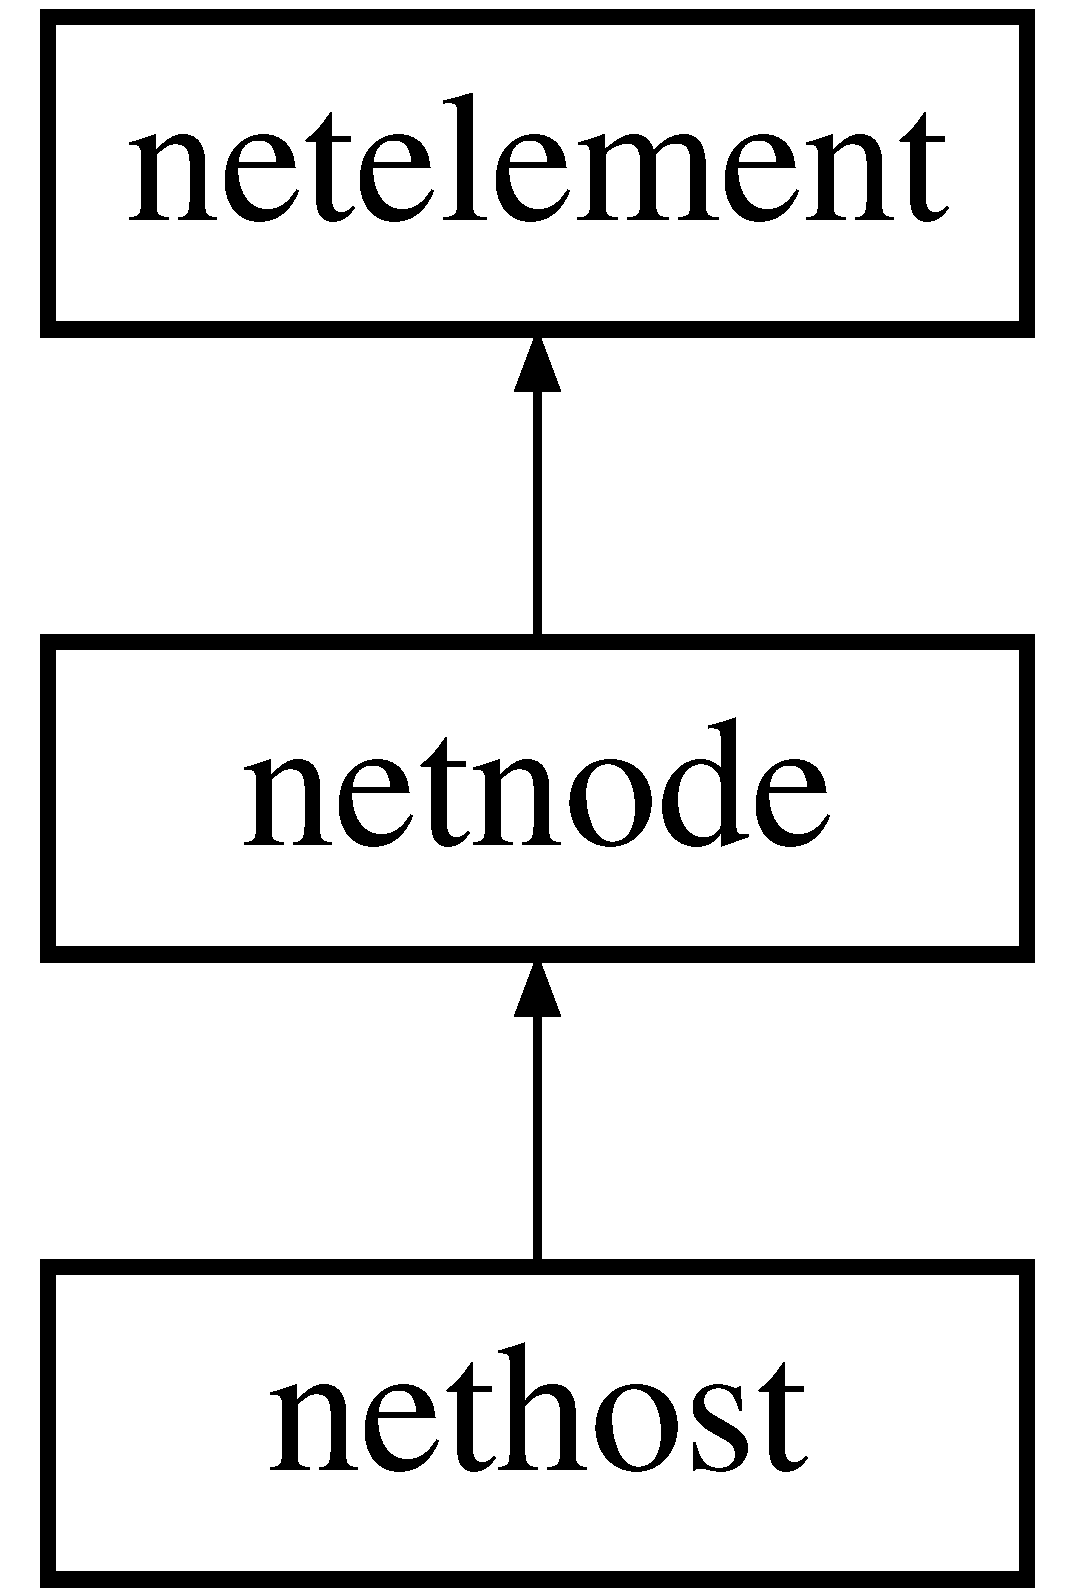
\includegraphics[height=3.000000cm]{classnethost}
\end{center}
\end{figure}
\subsection*{Public Member Functions}
\begin{DoxyCompactItemize}
\item 
\hyperlink{classnethost_aa5adfed919c8bf202bfba51b8cd68b34}{nethost} (string name)
\begin{DoxyCompactList}\small\item\em Sets the name to the given one and the nesting depth to 0 via the {\ttfamily netnode} constructor. \end{DoxyCompactList}\item 
\hyperlink{classnethost_ae13dd118e3f4e9f7892a3c8e733a1f48}{nethost} (string name, \hyperlink{classnetlink}{netlink} \&link)
\begin{DoxyCompactList}\small\item\em Sets the name to the given one and sets exactly one link for this host. \end{DoxyCompactList}\item 
bool \hyperlink{classnethost_ad1d207431110c8c254883cf02e8fd471}{is\-Routing\-Node} () const 
\begin{DoxyCompactList}\small\item\em Returns false because this is a host, not a router. \end{DoxyCompactList}\item 
\hyperlink{classnetlink}{netlink} $\ast$ \hyperlink{classnethost_a953214ef8b8de37f7db7a384a80a7b72}{get\-Link} () const 
\begin{DoxyCompactList}\small\item\em Gets the first (and only, since this is a host) link. \end{DoxyCompactList}\item 
void \hyperlink{classnethost_a9d374520690dd6fe8d04d68b330c41a1}{set\-Link} (\hyperlink{classnetlink}{netlink} \&link)
\begin{DoxyCompactList}\small\item\em Deletes all links then adds the given one. \end{DoxyCompactList}\item 
virtual void \hyperlink{classnethost_a1deafa5ff406d3b5d94d8fdf759a0951}{print\-Helper} (ostream \&os) const 
\begin{DoxyCompactList}\small\item\em Print helper function which partially overrides the one in {\ttfamily netdevice}. \end{DoxyCompactList}\end{DoxyCompactItemize}
\subsection*{Additional Inherited Members}


\subsection{Detailed Description}
Represents a host. 

The main difference between a {\ttfamily nethost} and a {\ttfamily netnode} is that a host can be attached to only one link. Hosts implement a selective A\-C\-K scheme; see the {\ttfamily received} field in {\ttfamily netflow}. 

\subsection{Constructor \& Destructor Documentation}
\hypertarget{classnethost_aa5adfed919c8bf202bfba51b8cd68b34}{\index{nethost@{nethost}!nethost@{nethost}}
\index{nethost@{nethost}!nethost@{nethost}}
\subsubsection[{nethost}]{\setlength{\rightskip}{0pt plus 5cm}nethost\-::nethost (
\begin{DoxyParamCaption}
\item[{string}]{name}
\end{DoxyParamCaption}
)}}\label{classnethost_aa5adfed919c8bf202bfba51b8cd68b34}


Sets the name to the given one and the nesting depth to 0 via the {\ttfamily netnode} constructor. 


\begin{DoxyParams}{Parameters}
{\em name} & of this host \\
\hline
\end{DoxyParams}
\hypertarget{classnethost_ae13dd118e3f4e9f7892a3c8e733a1f48}{\index{nethost@{nethost}!nethost@{nethost}}
\index{nethost@{nethost}!nethost@{nethost}}
\subsubsection[{nethost}]{\setlength{\rightskip}{0pt plus 5cm}nethost\-::nethost (
\begin{DoxyParamCaption}
\item[{string}]{name, }
\item[{{\bf netlink} \&}]{link}
\end{DoxyParamCaption}
)}}\label{classnethost_ae13dd118e3f4e9f7892a3c8e733a1f48}


Sets the name to the given one and sets exactly one link for this host. 


\begin{DoxyParams}{Parameters}
{\em name} & of this host \\
\hline
{\em link} & the only link that's attached to this host \\
\hline
\end{DoxyParams}


\subsection{Member Function Documentation}
\hypertarget{classnethost_a953214ef8b8de37f7db7a384a80a7b72}{\index{nethost@{nethost}!get\-Link@{get\-Link}}
\index{get\-Link@{get\-Link}!nethost@{nethost}}
\subsubsection[{get\-Link}]{\setlength{\rightskip}{0pt plus 5cm}{\bf netlink} $\ast$ nethost\-::get\-Link (
\begin{DoxyParamCaption}
{}
\end{DoxyParamCaption}
) const}}\label{classnethost_a953214ef8b8de37f7db7a384a80a7b72}


Gets the first (and only, since this is a host) link. 

\begin{DoxyReturn}{Returns}
link attached to this host 
\end{DoxyReturn}
\hypertarget{classnethost_ad1d207431110c8c254883cf02e8fd471}{\index{nethost@{nethost}!is\-Routing\-Node@{is\-Routing\-Node}}
\index{is\-Routing\-Node@{is\-Routing\-Node}!nethost@{nethost}}
\subsubsection[{is\-Routing\-Node}]{\setlength{\rightskip}{0pt plus 5cm}bool nethost\-::is\-Routing\-Node (
\begin{DoxyParamCaption}
{}
\end{DoxyParamCaption}
) const\hspace{0.3cm}{\ttfamily [virtual]}}}\label{classnethost_ad1d207431110c8c254883cf02e8fd471}


Returns false because this is a host, not a router. 

\begin{DoxyReturn}{Returns}
false 
\end{DoxyReturn}


Implements \hyperlink{classnetnode_a4a8b5169af7145506be0d31f6307908a}{netnode}.

\hypertarget{classnethost_a1deafa5ff406d3b5d94d8fdf759a0951}{\index{nethost@{nethost}!print\-Helper@{print\-Helper}}
\index{print\-Helper@{print\-Helper}!nethost@{nethost}}
\subsubsection[{print\-Helper}]{\setlength{\rightskip}{0pt plus 5cm}void nethost\-::print\-Helper (
\begin{DoxyParamCaption}
\item[{ostream \&}]{os}
\end{DoxyParamCaption}
) const\hspace{0.3cm}{\ttfamily [virtual]}}}\label{classnethost_a1deafa5ff406d3b5d94d8fdf759a0951}


Print helper function which partially overrides the one in {\ttfamily netdevice}. 


\begin{DoxyParams}{Parameters}
{\em os} & The output stream to which to write. \\
\hline
\end{DoxyParams}
\hypertarget{classnethost_a9d374520690dd6fe8d04d68b330c41a1}{\index{nethost@{nethost}!set\-Link@{set\-Link}}
\index{set\-Link@{set\-Link}!nethost@{nethost}}
\subsubsection[{set\-Link}]{\setlength{\rightskip}{0pt plus 5cm}void nethost\-::set\-Link (
\begin{DoxyParamCaption}
\item[{{\bf netlink} \&}]{link}
\end{DoxyParamCaption}
)}}\label{classnethost_a9d374520690dd6fe8d04d68b330c41a1}


Deletes all links then adds the given one. 


\begin{DoxyParams}{Parameters}
{\em link} & link to add after deleting the others \\
\hline
\end{DoxyParams}


The documentation for this class was generated from the following files\-:\begin{DoxyCompactItemize}
\item 
src/\hyperlink{network_8h}{network.\-h}\item 
src/network.\-cpp\end{DoxyCompactItemize}

\hypertarget{classnetlink}{\section{netlink Class Reference}
\label{classnetlink}\index{netlink@{netlink}}
}


Represents a half-\/duplex link.  




{\ttfamily \#include $<$network.\-h$>$}

Inheritance diagram for netlink\-:\begin{figure}[H]
\begin{center}
\leavevmode
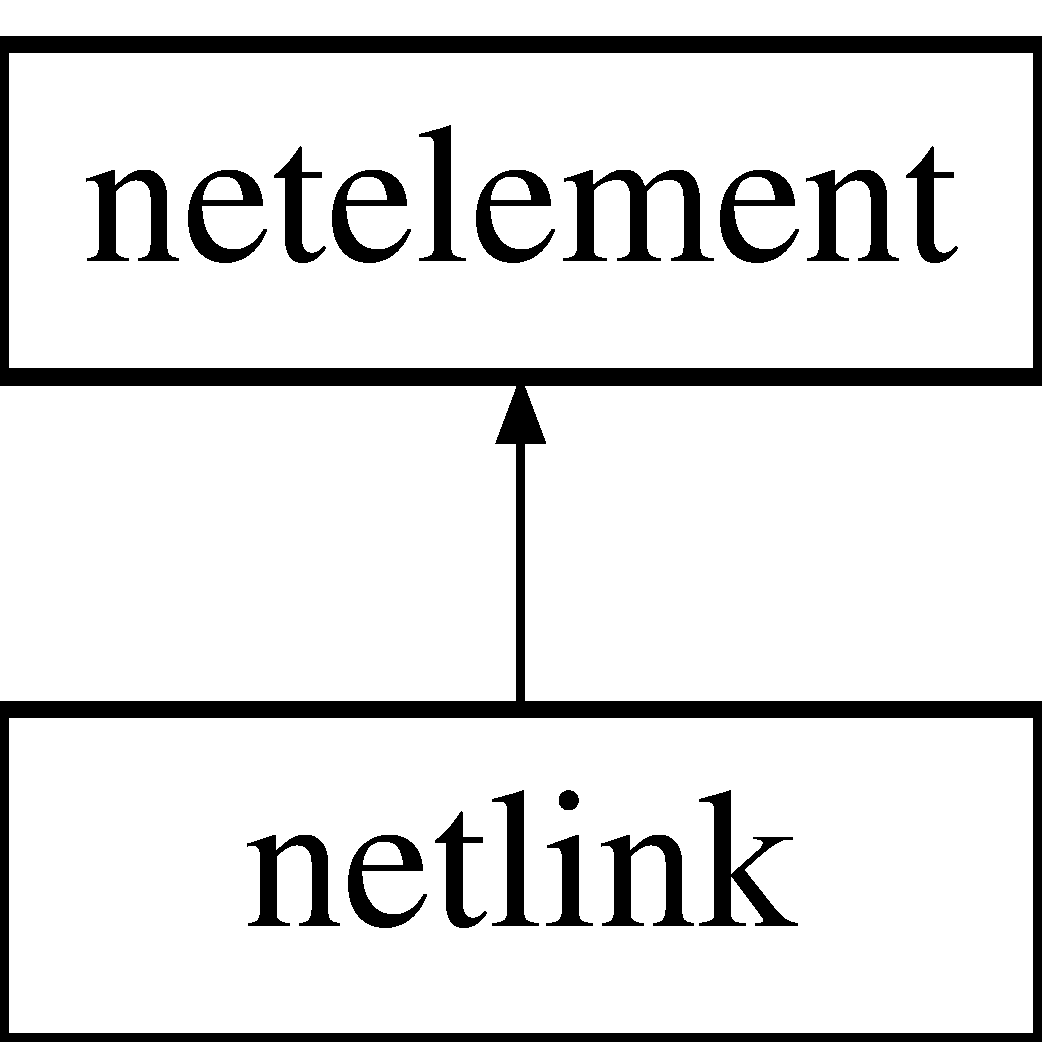
\includegraphics[height=2.000000cm]{classnetlink}
\end{center}
\end{figure}
\subsection*{Public Member Functions}
\begin{DoxyCompactItemize}
\item 
\hyperlink{classnetlink_a80fb314878612a849029c50ffaca2493}{netlink} (string name, double rate\-\_\-mbps, int delay\-\_\-ms, int buflen\-\_\-kb, \hyperlink{classnetnode}{netnode} \&endpoint1, \hyperlink{classnetnode}{netnode} \&endpoint2)
\begin{DoxyCompactList}\small\item\em Use this when endpoints are known at construction time. \end{DoxyCompactList}\item 
\hyperlink{classnetlink_ad82c705751d6eba3e0aee7cc51bc79ac}{netlink} (string name, double rate\-\_\-mbps, int delay\-\_\-ms, int buflen\-\_\-kb)
\begin{DoxyCompactList}\small\item\em Use this when endpoints are not known at construction time. \end{DoxyCompactList}\item 
long \hyperlink{classnetlink_abc9b2aa6e7f70d7c7c6d3db10ce4411e}{get\-Buflen} () const 
\begin{DoxyCompactList}\small\item\em Getter for the buffer's length in bytes (not occupancy). \end{DoxyCompactList}\item 
long \hyperlink{classnetlink_a620d116c9c81ba9acd3d6bddf26823e2}{get\-Buflen\-K\-B} () const 
\begin{DoxyCompactList}\small\item\em Getter for the buffer's length in kilobytes (not occupancy). \end{DoxyCompactList}\item 
int \hyperlink{classnetlink_acb7cdd8817ce85ce1c4a6641871f0768}{get\-Delay} () const 
\begin{DoxyCompactList}\small\item\em Getter for the link delay. \end{DoxyCompactList}\item 
\hyperlink{classnetnode}{netnode} $\ast$ \hyperlink{classnetlink_a3d479ae6579650a2137265132994c230}{get\-Endpoint1} () const 
\begin{DoxyCompactList}\small\item\em Getter for one of the endpoints that this link connects. \end{DoxyCompactList}\item 
\hyperlink{classnetnode}{netnode} $\ast$ \hyperlink{classnetlink_a94e8f2ac142cbf8f4d12ddba641d7f93}{get\-Endpoint2} () const 
\begin{DoxyCompactList}\small\item\em Getter for the other endpoint that this link connects. \end{DoxyCompactList}\item 
double \hyperlink{classnetlink_a67b47d5b1f4318769fa8f04af8496c79}{get\-Capacity\-Bits\-Per\-Sec} () const 
\begin{DoxyCompactList}\small\item\em Getter for the capacity of this link in bits per second. \end{DoxyCompactList}\item 
double \hyperlink{classnetlink_aa8a9e46c022c6be9078b1ffebe0c6083}{get\-Capacity\-Mbps} () const 
\begin{DoxyCompactList}\small\item\em Getter for the capacity of this link in megabits per second. \end{DoxyCompactList}\item 
double \hyperlink{classnetlink_a64822d2a7b2973f9bb3a8207798446d0}{get\-Rate\-Mbps} ()
\begin{DoxyCompactList}\small\item\em Getter for the current rate of the link in megabits per second. \end{DoxyCompactList}\item 
double \hyperlink{classnetlink_ae2cc1d19c2418172e5e36efd133deecb}{get\-Transmission\-Time\-Ms} (const \hyperlink{classpacket}{packet} \&pkt) const 
\begin{DoxyCompactList}\small\item\em Getter for end-\/to-\/end time in milliseconds for the given packet on this link N\-O\-T I\-N\-C\-L\-U\-D\-I\-N\-G D\-E\-L\-A\-Y. \end{DoxyCompactList}\item 
double \hyperlink{classnetlink_a20348993ebfa2fec8dbe30009e7d318d}{get\-Link\-Free\-At\-Time} () const 
\begin{DoxyCompactList}\small\item\em Getter for the absolute time in milliseconds when this link will be available for the next packet. \end{DoxyCompactList}\item 
long \hyperlink{classnetlink_a0fd7563496f463d8c044b8bf36a84cd8}{get\-Buffer\-Occupancy} () const 
\begin{DoxyCompactList}\small\item\em Getter for the number of bytes of the link buffer than are in-\/use. \end{DoxyCompactList}\item 
int \hyperlink{classnetlink_a16dda9d2d85bd71fd8ea610b4f9eccad}{get\-Pkt\-Loss} () const 
\begin{DoxyCompactList}\small\item\em Gette for the packet loss, which is number of packets dropped since we are assuming nothing happens to a packet while in transit. \end{DoxyCompactList}\item 
map$<$ string, int $>$ \hyperlink{classnetlink_a02c8a58b7691d074f2175bf4ef2cdb4b}{get\-Link\-Traffic} () const 
\begin{DoxyCompactList}\small\item\em Getter for the link traffic. \end{DoxyCompactList}\item 
bool \hyperlink{classnetlink_a4a44ff4a8b3fd1471f2b38d7c94dc48e}{is\-Same\-Direction\-As\-Last\-Packet} (\hyperlink{classnetnode}{netnode} $\ast$destination)
\begin{DoxyCompactList}\small\item\em This function is critical for our half-\/duplex implementation. \end{DoxyCompactList}\item 
double \hyperlink{classnetlink_a1af9572c35dadff0cf25621cbf1d31b0}{get\-Arrival\-Time} (const \hyperlink{classpacket}{packet} \&pkt, bool use\-Delay, double time)
\begin{DoxyCompactList}\small\item\em Gets the arrival time of a packet on the other end of the link. \end{DoxyCompactList}\item 
void \hyperlink{classnetlink_aea20be1cbfffa0ddc1dffa1b20be8305}{print\-Buffer} (ostream \&os)
\begin{DoxyCompactList}\small\item\em Prints the contents and size of the buffer to the given stream. \end{DoxyCompactList}\item 
virtual void \hyperlink{classnetlink_ade945f53c9730fcbeb3c3556da077d99}{print\-Helper} (ostream \&os) const 
\begin{DoxyCompactList}\small\item\em Print helper function which partially overrides the one in {\ttfamily netdevice}. \end{DoxyCompactList}\item 
void \hyperlink{classnetlink_ab92d2503ffd759aaf566bbc5c0f383d5}{set\-Endpoint1} (\hyperlink{classnetnode}{netnode} \&endpoint1)
\begin{DoxyCompactList}\small\item\em Setter for the first endpoint. \end{DoxyCompactList}\item 
void \hyperlink{classnetlink_a3e919ef44ab61692e5ff8af9bc08199d}{set\-Endpoint2} (\hyperlink{classnetnode}{netnode} \&endpoint2)
\begin{DoxyCompactList}\small\item\em Setter for the first endpoint. \end{DoxyCompactList}\item 
bool \hyperlink{classnetlink_ac0ccebbeb83abdbdc73533c29897250e}{send\-Packet} (const \hyperlink{classpacket}{packet} \&pkt, \hyperlink{classnetnode}{netnode} $\ast$destination, bool use\-Delay, double time)
\begin{DoxyCompactList}\small\item\em If the link buffer has space the given packet is added to the buffer and the rolling wait time and buffer occupancy are increased. \end{DoxyCompactList}\item 
bool \hyperlink{classnetlink_ad2f5311a0a1f6f0afc3667f3e1f1c0fe}{received\-Packet} (long pkt\-\_\-id)
\begin{DoxyCompactList}\small\item\em Called when a lone packet is received to free the link for subsequent packets; just dequeues the packet from the buffer. \end{DoxyCompactList}\item 
bool \hyperlink{classnetlink_ac345307525d371f1093b71d53665b8b7}{received\-Packet\-In\-Window} (long pkt\-\_\-id, bool first\-\_\-packet)
\begin{DoxyCompactList}\small\item\em Call this instead of {\ttfamily received\-Lone\-Packet} when an arriving packet is a part of a window so that the link buffer's wait time is adjusted correctly. \end{DoxyCompactList}\item 
\hypertarget{classnetlink_a354a84d64f26b8e1c811cac076967a4f}{void \hyperlink{classnetlink_a354a84d64f26b8e1c811cac076967a4f}{reset\-Link\-Traffic} ()}\label{classnetlink_a354a84d64f26b8e1c811cac076967a4f}

\begin{DoxyCompactList}\small\item\em Resets all values in link\-Traffic map to 0. \end{DoxyCompactList}\item 
void \hyperlink{classnetlink_a5100639202ca31e9459431e936ce5424}{update\-Link\-Traffic} (int time, \hyperlink{util_8h_ad875bcb78f9bd8625c5e454cafdc8de7}{packet\-\_\-type} type)
\begin{DoxyCompactList}\small\item\em Updates value of link\-Traffic accordingly. \end{DoxyCompactList}\end{DoxyCompactItemize}


\subsection{Detailed Description}
Represents a half-\/duplex link. 

\subsection{Constructor \& Destructor Documentation}
\hypertarget{classnetlink_a80fb314878612a849029c50ffaca2493}{\index{netlink@{netlink}!netlink@{netlink}}
\index{netlink@{netlink}!netlink@{netlink}}
\subsubsection[{netlink}]{\setlength{\rightskip}{0pt plus 5cm}netlink\-::netlink (
\begin{DoxyParamCaption}
\item[{string}]{name, }
\item[{double}]{rate\-\_\-mbps, }
\item[{int}]{delay\-\_\-ms, }
\item[{int}]{buflen\-\_\-kb, }
\item[{{\bf netnode} \&}]{endpoint1, }
\item[{{\bf netnode} \&}]{endpoint2}
\end{DoxyParamCaption}
)}}\label{classnetlink_a80fb314878612a849029c50ffaca2493}


Use this when endpoints are known at construction time. 


\begin{DoxyParams}{Parameters}
{\em name} & of this link \\
\hline
{\em rate\-\_\-mbps} & link rate in megabits per second \\
\hline
{\em delay\-\_\-ms} & link delay in milliseconds \\
\hline
{\em buflen\-\_\-kb} & the size of the only buffer on this link in kilobytes. This is stored internally in bytes. \\
\hline
{\em endpoint1} & the host or router on one side of this link \\
\hline
{\em endpoint2} & the host or router on the other side of this link \\
\hline
\end{DoxyParams}
\hypertarget{classnetlink_ad82c705751d6eba3e0aee7cc51bc79ac}{\index{netlink@{netlink}!netlink@{netlink}}
\index{netlink@{netlink}!netlink@{netlink}}
\subsubsection[{netlink}]{\setlength{\rightskip}{0pt plus 5cm}netlink\-::netlink (
\begin{DoxyParamCaption}
\item[{string}]{name, }
\item[{double}]{rate\-\_\-mbps, }
\item[{int}]{delay\-\_\-ms, }
\item[{int}]{buflen\-\_\-kb}
\end{DoxyParamCaption}
)}}\label{classnetlink_ad82c705751d6eba3e0aee7cc51bc79ac}


Use this when endpoints are not known at construction time. 


\begin{DoxyParams}{Parameters}
{\em name} & of this link \\
\hline
{\em rate\-\_\-mbps} & link rate in megabits per second \\
\hline
{\em delay\-\_\-ms} & link delay in milliseconds \\
\hline
{\em buflen\-\_\-kb} & the size of the only buffer on this link in kilobytes This is stored internally in bytes. \\
\hline
\end{DoxyParams}


\subsection{Member Function Documentation}
\hypertarget{classnetlink_a1af9572c35dadff0cf25621cbf1d31b0}{\index{netlink@{netlink}!get\-Arrival\-Time@{get\-Arrival\-Time}}
\index{get\-Arrival\-Time@{get\-Arrival\-Time}!netlink@{netlink}}
\subsubsection[{get\-Arrival\-Time}]{\setlength{\rightskip}{0pt plus 5cm}double netlink\-::get\-Arrival\-Time (
\begin{DoxyParamCaption}
\item[{const {\bf packet} \&}]{pkt, }
\item[{bool}]{use\-Delay, }
\item[{double}]{time}
\end{DoxyParamCaption}
)}}\label{classnetlink_a1af9572c35dadff0cf25621cbf1d31b0}


Gets the arrival time of a packet on the other end of the link. 


\begin{DoxyParams}{Parameters}
{\em pkt} & \\
\hline
{\em use\-Delay} & \\
\hline
{\em time} & of the triggered event \\
\hline
\end{DoxyParams}
\begin{DoxyReturn}{Returns}
arrival time 
\end{DoxyReturn}
\hypertarget{classnetlink_a0fd7563496f463d8c044b8bf36a84cd8}{\index{netlink@{netlink}!get\-Buffer\-Occupancy@{get\-Buffer\-Occupancy}}
\index{get\-Buffer\-Occupancy@{get\-Buffer\-Occupancy}!netlink@{netlink}}
\subsubsection[{get\-Buffer\-Occupancy}]{\setlength{\rightskip}{0pt plus 5cm}long netlink\-::get\-Buffer\-Occupancy (
\begin{DoxyParamCaption}
{}
\end{DoxyParamCaption}
) const}}\label{classnetlink_a0fd7563496f463d8c044b8bf36a84cd8}


Getter for the number of bytes of the link buffer than are in-\/use. 

\begin{DoxyReturn}{Returns}
the buffer occupancy (bytes) 
\end{DoxyReturn}
\hypertarget{classnetlink_abc9b2aa6e7f70d7c7c6d3db10ce4411e}{\index{netlink@{netlink}!get\-Buflen@{get\-Buflen}}
\index{get\-Buflen@{get\-Buflen}!netlink@{netlink}}
\subsubsection[{get\-Buflen}]{\setlength{\rightskip}{0pt plus 5cm}long netlink\-::get\-Buflen (
\begin{DoxyParamCaption}
{}
\end{DoxyParamCaption}
) const}}\label{classnetlink_abc9b2aa6e7f70d7c7c6d3db10ce4411e}


Getter for the buffer's length in bytes (not occupancy). 

\begin{DoxyReturn}{Returns}
buffer length in bytes. 
\end{DoxyReturn}
\hypertarget{classnetlink_a620d116c9c81ba9acd3d6bddf26823e2}{\index{netlink@{netlink}!get\-Buflen\-K\-B@{get\-Buflen\-K\-B}}
\index{get\-Buflen\-K\-B@{get\-Buflen\-K\-B}!netlink@{netlink}}
\subsubsection[{get\-Buflen\-K\-B}]{\setlength{\rightskip}{0pt plus 5cm}long netlink\-::get\-Buflen\-K\-B (
\begin{DoxyParamCaption}
{}
\end{DoxyParamCaption}
) const}}\label{classnetlink_a620d116c9c81ba9acd3d6bddf26823e2}


Getter for the buffer's length in kilobytes (not occupancy). 

\begin{DoxyReturn}{Returns}
buffer length in k\-B. 
\end{DoxyReturn}
\hypertarget{classnetlink_a67b47d5b1f4318769fa8f04af8496c79}{\index{netlink@{netlink}!get\-Capacity\-Bits\-Per\-Sec@{get\-Capacity\-Bits\-Per\-Sec}}
\index{get\-Capacity\-Bits\-Per\-Sec@{get\-Capacity\-Bits\-Per\-Sec}!netlink@{netlink}}
\subsubsection[{get\-Capacity\-Bits\-Per\-Sec}]{\setlength{\rightskip}{0pt plus 5cm}double netlink\-::get\-Capacity\-Bits\-Per\-Sec (
\begin{DoxyParamCaption}
{}
\end{DoxyParamCaption}
) const}}\label{classnetlink_a67b47d5b1f4318769fa8f04af8496c79}


Getter for the capacity of this link in bits per second. 

\begin{DoxyReturn}{Returns}
link capacity (bps) 
\end{DoxyReturn}
\hypertarget{classnetlink_aa8a9e46c022c6be9078b1ffebe0c6083}{\index{netlink@{netlink}!get\-Capacity\-Mbps@{get\-Capacity\-Mbps}}
\index{get\-Capacity\-Mbps@{get\-Capacity\-Mbps}!netlink@{netlink}}
\subsubsection[{get\-Capacity\-Mbps}]{\setlength{\rightskip}{0pt plus 5cm}double netlink\-::get\-Capacity\-Mbps (
\begin{DoxyParamCaption}
{}
\end{DoxyParamCaption}
) const}}\label{classnetlink_aa8a9e46c022c6be9078b1ffebe0c6083}


Getter for the capacity of this link in megabits per second. 

\begin{DoxyReturn}{Returns}
link capacity (mbps) 
\end{DoxyReturn}
\hypertarget{classnetlink_acb7cdd8817ce85ce1c4a6641871f0768}{\index{netlink@{netlink}!get\-Delay@{get\-Delay}}
\index{get\-Delay@{get\-Delay}!netlink@{netlink}}
\subsubsection[{get\-Delay}]{\setlength{\rightskip}{0pt plus 5cm}int netlink\-::get\-Delay (
\begin{DoxyParamCaption}
{}
\end{DoxyParamCaption}
) const}}\label{classnetlink_acb7cdd8817ce85ce1c4a6641871f0768}


Getter for the link delay. 

\begin{DoxyReturn}{Returns}
delay in milliseconds. 
\end{DoxyReturn}
\hypertarget{classnetlink_a3d479ae6579650a2137265132994c230}{\index{netlink@{netlink}!get\-Endpoint1@{get\-Endpoint1}}
\index{get\-Endpoint1@{get\-Endpoint1}!netlink@{netlink}}
\subsubsection[{get\-Endpoint1}]{\setlength{\rightskip}{0pt plus 5cm}{\bf netnode} $\ast$ netlink\-::get\-Endpoint1 (
\begin{DoxyParamCaption}
{}
\end{DoxyParamCaption}
) const}}\label{classnetlink_a3d479ae6579650a2137265132994c230}


Getter for one of the endpoints that this link connects. 

This might be a node or a router. \begin{DoxyReturn}{Returns}
one of the endpoints 
\end{DoxyReturn}
\hypertarget{classnetlink_a94e8f2ac142cbf8f4d12ddba641d7f93}{\index{netlink@{netlink}!get\-Endpoint2@{get\-Endpoint2}}
\index{get\-Endpoint2@{get\-Endpoint2}!netlink@{netlink}}
\subsubsection[{get\-Endpoint2}]{\setlength{\rightskip}{0pt plus 5cm}{\bf netnode} $\ast$ netlink\-::get\-Endpoint2 (
\begin{DoxyParamCaption}
{}
\end{DoxyParamCaption}
) const}}\label{classnetlink_a94e8f2ac142cbf8f4d12ddba641d7f93}


Getter for the other endpoint that this link connects. 

This might be a node or a router. \begin{DoxyReturn}{Returns}
the other endpoint 
\end{DoxyReturn}
\hypertarget{classnetlink_a20348993ebfa2fec8dbe30009e7d318d}{\index{netlink@{netlink}!get\-Link\-Free\-At\-Time@{get\-Link\-Free\-At\-Time}}
\index{get\-Link\-Free\-At\-Time@{get\-Link\-Free\-At\-Time}!netlink@{netlink}}
\subsubsection[{get\-Link\-Free\-At\-Time}]{\setlength{\rightskip}{0pt plus 5cm}double netlink\-::get\-Link\-Free\-At\-Time (
\begin{DoxyParamCaption}
{}
\end{DoxyParamCaption}
) const}}\label{classnetlink_a20348993ebfa2fec8dbe30009e7d318d}


Getter for the absolute time in milliseconds when this link will be available for the next packet. 

\begin{DoxyReturn}{Returns}
time at which link will be available for next-\/queued packet 
\end{DoxyReturn}
\begin{DoxyWarning}{Warning}
if zero need to substitute current time in for free at time! the link doesn't know the current time, so it can't tell you when the link is free if there's nothing in the buffer. 
\end{DoxyWarning}
\hypertarget{classnetlink_a02c8a58b7691d074f2175bf4ef2cdb4b}{\index{netlink@{netlink}!get\-Link\-Traffic@{get\-Link\-Traffic}}
\index{get\-Link\-Traffic@{get\-Link\-Traffic}!netlink@{netlink}}
\subsubsection[{get\-Link\-Traffic}]{\setlength{\rightskip}{0pt plus 5cm}map$<$ string, int $>$ netlink\-::get\-Link\-Traffic (
\begin{DoxyParamCaption}
{}
\end{DoxyParamCaption}
) const}}\label{classnetlink_a02c8a58b7691d074f2175bf4ef2cdb4b}


Getter for the link traffic. 

\begin{DoxyReturn}{Returns}
link\-Traffic 
\end{DoxyReturn}
\hypertarget{classnetlink_a16dda9d2d85bd71fd8ea610b4f9eccad}{\index{netlink@{netlink}!get\-Pkt\-Loss@{get\-Pkt\-Loss}}
\index{get\-Pkt\-Loss@{get\-Pkt\-Loss}!netlink@{netlink}}
\subsubsection[{get\-Pkt\-Loss}]{\setlength{\rightskip}{0pt plus 5cm}int netlink\-::get\-Pkt\-Loss (
\begin{DoxyParamCaption}
{}
\end{DoxyParamCaption}
) const}}\label{classnetlink_a16dda9d2d85bd71fd8ea610b4f9eccad}


Gette for the packet loss, which is number of packets dropped since we are assuming nothing happens to a packet while in transit. 

\begin{DoxyReturn}{Returns}
packet loss 
\end{DoxyReturn}
\hypertarget{classnetlink_a64822d2a7b2973f9bb3a8207798446d0}{\index{netlink@{netlink}!get\-Rate\-Mbps@{get\-Rate\-Mbps}}
\index{get\-Rate\-Mbps@{get\-Rate\-Mbps}!netlink@{netlink}}
\subsubsection[{get\-Rate\-Mbps}]{\setlength{\rightskip}{0pt plus 5cm}double netlink\-::get\-Rate\-Mbps (
\begin{DoxyParamCaption}
{}
\end{DoxyParamCaption}
)}}\label{classnetlink_a64822d2a7b2973f9bb3a8207798446d0}


Getter for the current rate of the link in megabits per second. 

\begin{DoxyReturn}{Returns}
current link rate (mbps) 
\end{DoxyReturn}
\hypertarget{classnetlink_ae2cc1d19c2418172e5e36efd133deecb}{\index{netlink@{netlink}!get\-Transmission\-Time\-Ms@{get\-Transmission\-Time\-Ms}}
\index{get\-Transmission\-Time\-Ms@{get\-Transmission\-Time\-Ms}!netlink@{netlink}}
\subsubsection[{get\-Transmission\-Time\-Ms}]{\setlength{\rightskip}{0pt plus 5cm}double netlink\-::get\-Transmission\-Time\-Ms (
\begin{DoxyParamCaption}
\item[{const {\bf packet} \&}]{pkt}
\end{DoxyParamCaption}
) const}}\label{classnetlink_ae2cc1d19c2418172e5e36efd133deecb}


Getter for end-\/to-\/end time in milliseconds for the given packet on this link N\-O\-T I\-N\-C\-L\-U\-D\-I\-N\-G D\-E\-L\-A\-Y. 


\begin{DoxyParams}{Parameters}
{\em pkt} & \\
\hline
\end{DoxyParams}
\begin{DoxyReturn}{Returns}
end-\/to-\/end time for this packet (ms) 
\end{DoxyReturn}
\hypertarget{classnetlink_a4a44ff4a8b3fd1471f2b38d7c94dc48e}{\index{netlink@{netlink}!is\-Same\-Direction\-As\-Last\-Packet@{is\-Same\-Direction\-As\-Last\-Packet}}
\index{is\-Same\-Direction\-As\-Last\-Packet@{is\-Same\-Direction\-As\-Last\-Packet}!netlink@{netlink}}
\subsubsection[{is\-Same\-Direction\-As\-Last\-Packet}]{\setlength{\rightskip}{0pt plus 5cm}bool netlink\-::is\-Same\-Direction\-As\-Last\-Packet (
\begin{DoxyParamCaption}
\item[{{\bf netnode} $\ast$}]{destination}
\end{DoxyParamCaption}
)}}\label{classnetlink_a4a44ff4a8b3fd1471f2b38d7c94dc48e}


This function is critical for our half-\/duplex implementation. 

Returns true if the direction of the last packet in the buffer is the same as the direction of the packet about to be added; if the direction is the same then the link delay should not be used, since it was already used once for the first packet in this run of same-\/direction packets. 
\begin{DoxyParams}{Parameters}
{\em destination} & \\
\hline
\end{DoxyParams}
\begin{DoxyReturn}{Returns}
true if the destination is the same as the destination of the last packet in the buffer 
\end{DoxyReturn}
\hypertarget{classnetlink_aea20be1cbfffa0ddc1dffa1b20be8305}{\index{netlink@{netlink}!print\-Buffer@{print\-Buffer}}
\index{print\-Buffer@{print\-Buffer}!netlink@{netlink}}
\subsubsection[{print\-Buffer}]{\setlength{\rightskip}{0pt plus 5cm}void netlink\-::print\-Buffer (
\begin{DoxyParamCaption}
\item[{ostream \&}]{os}
\end{DoxyParamCaption}
)}}\label{classnetlink_aea20be1cbfffa0ddc1dffa1b20be8305}


Prints the contents and size of the buffer to the given stream. 

Extremely useful for debugging. 
\begin{DoxyParams}{Parameters}
{\em os} & print the buffer contents to this output stream. \\
\hline
\end{DoxyParams}
\hypertarget{classnetlink_ade945f53c9730fcbeb3c3556da077d99}{\index{netlink@{netlink}!print\-Helper@{print\-Helper}}
\index{print\-Helper@{print\-Helper}!netlink@{netlink}}
\subsubsection[{print\-Helper}]{\setlength{\rightskip}{0pt plus 5cm}void netlink\-::print\-Helper (
\begin{DoxyParamCaption}
\item[{ostream \&}]{os}
\end{DoxyParamCaption}
) const\hspace{0.3cm}{\ttfamily [virtual]}}}\label{classnetlink_ade945f53c9730fcbeb3c3556da077d99}


Print helper function which partially overrides the one in {\ttfamily netdevice}. 


\begin{DoxyParams}{Parameters}
{\em os} & The output stream to which to write. \\
\hline
\end{DoxyParams}
\hypertarget{classnetlink_ad2f5311a0a1f6f0afc3667f3e1f1c0fe}{\index{netlink@{netlink}!received\-Packet@{received\-Packet}}
\index{received\-Packet@{received\-Packet}!netlink@{netlink}}
\subsubsection[{received\-Packet}]{\setlength{\rightskip}{0pt plus 5cm}bool netlink\-::received\-Packet (
\begin{DoxyParamCaption}
\item[{long}]{pkt\-\_\-id}
\end{DoxyParamCaption}
)}}\label{classnetlink_ad2f5311a0a1f6f0afc3667f3e1f1c0fe}


Called when a lone packet is received to free the link for subsequent packets; just dequeues the packet from the buffer. 


\begin{DoxyParams}{Parameters}
{\em pkt\-\_\-id} & the given packet I\-D number must match the I\-D of the packet about to be dequeued.\\
\hline
\end{DoxyParams}
\begin{DoxyReturn}{Returns}
true if the packet was dequeued (i.\-e. the given id matched and the buffer wasn't empty) 
\end{DoxyReturn}
\hypertarget{classnetlink_ac345307525d371f1093b71d53665b8b7}{\index{netlink@{netlink}!received\-Packet\-In\-Window@{received\-Packet\-In\-Window}}
\index{received\-Packet\-In\-Window@{received\-Packet\-In\-Window}!netlink@{netlink}}
\subsubsection[{received\-Packet\-In\-Window}]{\setlength{\rightskip}{0pt plus 5cm}bool netlink\-::received\-Packet\-In\-Window (
\begin{DoxyParamCaption}
\item[{long}]{pkt\-\_\-id, }
\item[{bool}]{first\-\_\-packet}
\end{DoxyParamCaption}
)}}\label{classnetlink_ac345307525d371f1093b71d53665b8b7}


Call this instead of {\ttfamily received\-Lone\-Packet} when an arriving packet is a part of a window so that the link buffer's wait time is adjusted correctly. 

For the first packet in a windowload the buffer's wait time is decreasing by the link delay + one transmission time, but for subsequent packets the buffer wait time is decreased by only one transmission time.


\begin{DoxyParams}{Parameters}
{\em pkt\-\_\-id} & the given packet I\-D number must match the I\-D of the packet about to be dequeued. \\
\hline
{\em first\-\_\-packet} & true if first packet in the window\\
\hline
\end{DoxyParams}
\begin{DoxyReturn}{Returns}
true if the packet was dequeued (i.\-e. the given id matched and the buffer wasn't empty) 
\end{DoxyReturn}
\hypertarget{classnetlink_ac0ccebbeb83abdbdc73533c29897250e}{\index{netlink@{netlink}!send\-Packet@{send\-Packet}}
\index{send\-Packet@{send\-Packet}!netlink@{netlink}}
\subsubsection[{send\-Packet}]{\setlength{\rightskip}{0pt plus 5cm}bool netlink\-::send\-Packet (
\begin{DoxyParamCaption}
\item[{const {\bf packet} \&}]{pkt, }
\item[{{\bf netnode} $\ast$}]{destination, }
\item[{bool}]{use\-Delay, }
\item[{double}]{time}
\end{DoxyParamCaption}
)}}\label{classnetlink_ac0ccebbeb83abdbdc73533c29897250e}


If the link buffer has space the given packet is added to the buffer and the rolling wait time and buffer occupancy are increased. 


\begin{DoxyParams}{Parameters}
{\em pkt} & the packet to add to the buffer \\
\hline
{\em destination} & of the packet \\
\hline
{\em use\-Delay} & true if link delay should be used to sum into the buffer's wait time. Should be used O\-N\-C\-E per window \\
\hline
{\em time} & at which we're trying to send this packet\\
\hline
\end{DoxyParams}
\begin{DoxyReturn}{Returns}
true if added to buffer successfully, false if dropped 
\end{DoxyReturn}
\hypertarget{classnetlink_ab92d2503ffd759aaf566bbc5c0f383d5}{\index{netlink@{netlink}!set\-Endpoint1@{set\-Endpoint1}}
\index{set\-Endpoint1@{set\-Endpoint1}!netlink@{netlink}}
\subsubsection[{set\-Endpoint1}]{\setlength{\rightskip}{0pt plus 5cm}void netlink\-::set\-Endpoint1 (
\begin{DoxyParamCaption}
\item[{{\bf netnode} \&}]{endpoint1}
\end{DoxyParamCaption}
)}}\label{classnetlink_ab92d2503ffd759aaf566bbc5c0f383d5}


Setter for the first endpoint. 


\begin{DoxyParams}{Parameters}
{\em endpoint1} & \\
\hline
\end{DoxyParams}
\hypertarget{classnetlink_a3e919ef44ab61692e5ff8af9bc08199d}{\index{netlink@{netlink}!set\-Endpoint2@{set\-Endpoint2}}
\index{set\-Endpoint2@{set\-Endpoint2}!netlink@{netlink}}
\subsubsection[{set\-Endpoint2}]{\setlength{\rightskip}{0pt plus 5cm}void netlink\-::set\-Endpoint2 (
\begin{DoxyParamCaption}
\item[{{\bf netnode} \&}]{endpoint2}
\end{DoxyParamCaption}
)}}\label{classnetlink_a3e919ef44ab61692e5ff8af9bc08199d}


Setter for the first endpoint. 


\begin{DoxyParams}{Parameters}
{\em endpoint1} & \\
\hline
\end{DoxyParams}
\hypertarget{classnetlink_a5100639202ca31e9459431e936ce5424}{\index{netlink@{netlink}!update\-Link\-Traffic@{update\-Link\-Traffic}}
\index{update\-Link\-Traffic@{update\-Link\-Traffic}!netlink@{netlink}}
\subsubsection[{update\-Link\-Traffic}]{\setlength{\rightskip}{0pt plus 5cm}void netlink\-::update\-Link\-Traffic (
\begin{DoxyParamCaption}
\item[{int}]{time, }
\item[{{\bf packet\-\_\-type}}]{type}
\end{DoxyParamCaption}
)}}\label{classnetlink_a5100639202ca31e9459431e936ce5424}


Updates value of link\-Traffic accordingly. 


\begin{DoxyParams}{Parameters}
{\em time} & \\
\hline
{\em type} & \\
\hline
\end{DoxyParams}


The documentation for this class was generated from the following files\-:\begin{DoxyCompactItemize}
\item 
src/\hyperlink{network_8h}{network.\-h}\item 
src/network.\-cpp\end{DoxyCompactItemize}

\hypertarget{classnetnode}{\section{netnode Class Reference}
\label{classnetnode}\index{netnode@{netnode}}
}


Represents a node, which is either a node or a host, in a simple network.  




{\ttfamily \#include $<$network.\-h$>$}

Inheritance diagram for netnode\-:\begin{figure}[H]
\begin{center}
\leavevmode
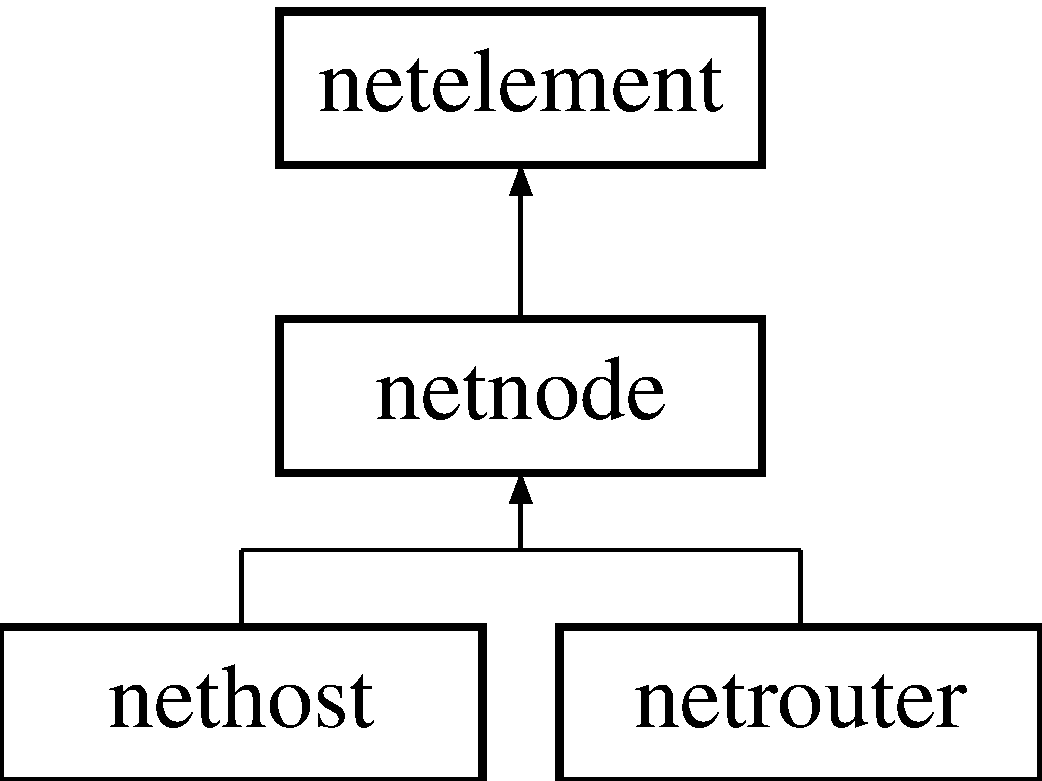
\includegraphics[height=3.000000cm]{classnetnode}
\end{center}
\end{figure}
\subsection*{Public Member Functions}
\begin{DoxyCompactItemize}
\item 
\hyperlink{classnetnode_ad0f9b3efbaa334595b62486d6dd419cf}{netnode} ()
\begin{DoxyCompactList}\small\item\em Default constructor. \end{DoxyCompactList}\item 
\hyperlink{classnetnode_a32eddc0b4bee9b523a6bffda4ef921ea}{netnode} (string name)
\begin{DoxyCompactList}\small\item\em Sets name to the given value and calls netelement's constuctor. \end{DoxyCompactList}\item 
\hyperlink{classnetnode_a8cf0f8e17de9aad66998a184adf96621}{netnode} (string name, vector$<$ \hyperlink{classnetlink}{netlink} $\ast$ $>$ \hyperlink{classnetnode_af481c4109393b79170f523ca92bea507}{links})
\begin{DoxyCompactList}\small\item\em Sets the name of this device to the given one and copies the list of given link pointers into this object's list of links. \end{DoxyCompactList}\item 
\hyperlink{classnetnode}{netnode} $\ast$ \hyperlink{classnetnode_a0af8d29fc1c1979fec8af2831e2bcc82}{get\-Other\-Node} (\hyperlink{classnetlink}{netlink} $\ast$link)
\begin{DoxyCompactList}\small\item\em Returns the node connected to the input link that is not $\ast$this node. \end{DoxyCompactList}\item 
virtual void \hyperlink{classnetnode_a4faaedd2e9121270a220eb67004dba7c}{add\-Link} (\hyperlink{classnetlink}{netlink} \&link)
\begin{DoxyCompactList}\small\item\em Mutator that adds links to this device's list of links. \end{DoxyCompactList}\item 
const vector$<$ \hyperlink{classnetlink}{netlink} $\ast$ $>$ \& \hyperlink{classnetnode_a0299d9b8d9bd8b12ea644fcd04359d1a}{get\-Links} () const 
\begin{DoxyCompactList}\small\item\em Getter for the list of links attached to this device. \end{DoxyCompactList}\item 
virtual bool \hyperlink{classnetnode_a4a8b5169af7145506be0d31f6307908a}{is\-Routing\-Node} () const =0
\begin{DoxyCompactList}\small\item\em Should be defined so this function returns true for packet-\/routers and false for packet-\/consumers. \end{DoxyCompactList}\item 
virtual void \hyperlink{classnetnode_acf1330a7d57a1358064b3736b888b464}{print\-Helper} (std\-::ostream \&os) const 
\begin{DoxyCompactList}\small\item\em Print helper function. \end{DoxyCompactList}\end{DoxyCompactItemize}
\subsection*{Protected Attributes}
\begin{DoxyCompactItemize}
\item 
vector$<$ \hyperlink{classnetlink}{netlink} $\ast$ $>$ \hyperlink{classnetnode_af481c4109393b79170f523ca92bea507}{links}
\begin{DoxyCompactList}\small\item\em Pointers to all the links attached to this node. \end{DoxyCompactList}\end{DoxyCompactItemize}


\subsection{Detailed Description}
Represents a node, which is either a node or a host, in a simple network. 

\subsection{Constructor \& Destructor Documentation}
\hypertarget{classnetnode_ad0f9b3efbaa334595b62486d6dd419cf}{\index{netnode@{netnode}!netnode@{netnode}}
\index{netnode@{netnode}!netnode@{netnode}}
\subsubsection[{netnode}]{\setlength{\rightskip}{0pt plus 5cm}netnode\-::netnode (
\begin{DoxyParamCaption}
{}
\end{DoxyParamCaption}
)}}\label{classnetnode_ad0f9b3efbaa334595b62486d6dd419cf}


Default constructor. 

\hypertarget{classnetnode_a32eddc0b4bee9b523a6bffda4ef921ea}{\index{netnode@{netnode}!netnode@{netnode}}
\index{netnode@{netnode}!netnode@{netnode}}
\subsubsection[{netnode}]{\setlength{\rightskip}{0pt plus 5cm}netnode\-::netnode (
\begin{DoxyParamCaption}
\item[{string}]{name}
\end{DoxyParamCaption}
)}}\label{classnetnode_a32eddc0b4bee9b523a6bffda4ef921ea}


Sets name to the given value and calls netelement's constuctor. 


\begin{DoxyParams}{Parameters}
{\em name} & of this device \\
\hline
\end{DoxyParams}
\hypertarget{classnetnode_a8cf0f8e17de9aad66998a184adf96621}{\index{netnode@{netnode}!netnode@{netnode}}
\index{netnode@{netnode}!netnode@{netnode}}
\subsubsection[{netnode}]{\setlength{\rightskip}{0pt plus 5cm}netnode\-::netnode (
\begin{DoxyParamCaption}
\item[{string}]{name, }
\item[{vector$<$ {\bf netlink} $\ast$ $>$}]{links}
\end{DoxyParamCaption}
)}}\label{classnetnode_a8cf0f8e17de9aad66998a184adf96621}


Sets the name of this device to the given one and copies the list of given link pointers into this object's list of links. 


\begin{DoxyParams}{Parameters}
{\em name} & of this device \\
\hline
{\em links} & vector of pointers to links attached to this device \\
\hline
\end{DoxyParams}


\subsection{Member Function Documentation}
\hypertarget{classnetnode_a4faaedd2e9121270a220eb67004dba7c}{\index{netnode@{netnode}!add\-Link@{add\-Link}}
\index{add\-Link@{add\-Link}!netnode@{netnode}}
\subsubsection[{add\-Link}]{\setlength{\rightskip}{0pt plus 5cm}void netnode\-::add\-Link (
\begin{DoxyParamCaption}
\item[{{\bf netlink} \&}]{link}
\end{DoxyParamCaption}
)\hspace{0.3cm}{\ttfamily [virtual]}}}\label{classnetnode_a4faaedd2e9121270a220eb67004dba7c}


Mutator that adds links to this device's list of links. 


\begin{DoxyParams}{Parameters}
{\em link} & to add to this device's list of links \\
\hline
\end{DoxyParams}
\hypertarget{classnetnode_a0299d9b8d9bd8b12ea644fcd04359d1a}{\index{netnode@{netnode}!get\-Links@{get\-Links}}
\index{get\-Links@{get\-Links}!netnode@{netnode}}
\subsubsection[{get\-Links}]{\setlength{\rightskip}{0pt plus 5cm}const vector$<$ {\bf netlink} $\ast$ $>$ \& netnode\-::get\-Links (
\begin{DoxyParamCaption}
{}
\end{DoxyParamCaption}
) const}}\label{classnetnode_a0299d9b8d9bd8b12ea644fcd04359d1a}


Getter for the list of links attached to this device. 

\begin{DoxyReturn}{Returns}
the list of links attached to this device 
\end{DoxyReturn}
\hypertarget{classnetnode_a0af8d29fc1c1979fec8af2831e2bcc82}{\index{netnode@{netnode}!get\-Other\-Node@{get\-Other\-Node}}
\index{get\-Other\-Node@{get\-Other\-Node}!netnode@{netnode}}
\subsubsection[{get\-Other\-Node}]{\setlength{\rightskip}{0pt plus 5cm}{\bf netnode} $\ast$ netnode\-::get\-Other\-Node (
\begin{DoxyParamCaption}
\item[{{\bf netlink} $\ast$}]{link}
\end{DoxyParamCaption}
)}}\label{classnetnode_a0af8d29fc1c1979fec8af2831e2bcc82}


Returns the node connected to the input link that is not $\ast$this node. 


\begin{DoxyParams}{Parameters}
{\em link} & get the node at the other end of this link \\
\hline
\end{DoxyParams}
\begin{DoxyReturn}{Returns}
pointer to the node at the other end of this link 
\end{DoxyReturn}
\hypertarget{classnetnode_a4a8b5169af7145506be0d31f6307908a}{\index{netnode@{netnode}!is\-Routing\-Node@{is\-Routing\-Node}}
\index{is\-Routing\-Node@{is\-Routing\-Node}!netnode@{netnode}}
\subsubsection[{is\-Routing\-Node}]{\setlength{\rightskip}{0pt plus 5cm}bool netnode\-::is\-Routing\-Node (
\begin{DoxyParamCaption}
{}
\end{DoxyParamCaption}
) const\hspace{0.3cm}{\ttfamily [pure virtual]}}}\label{classnetnode_a4a8b5169af7145506be0d31f6307908a}


Should be defined so this function returns true for packet-\/routers and false for packet-\/consumers. 

\begin{DoxyReturn}{Returns}
true if this node is capable of routing packets. 
\end{DoxyReturn}


Implemented in \hyperlink{classnetrouter_a1fa1b2262b7427485b31b2d90477b6e7}{netrouter}, and \hyperlink{classnethost_ad1d207431110c8c254883cf02e8fd471}{nethost}.

\hypertarget{classnetnode_acf1330a7d57a1358064b3736b888b464}{\index{netnode@{netnode}!print\-Helper@{print\-Helper}}
\index{print\-Helper@{print\-Helper}!netnode@{netnode}}
\subsubsection[{print\-Helper}]{\setlength{\rightskip}{0pt plus 5cm}void netnode\-::print\-Helper (
\begin{DoxyParamCaption}
\item[{std\-::ostream \&}]{os}
\end{DoxyParamCaption}
) const\hspace{0.3cm}{\ttfamily [virtual]}}}\label{classnetnode_acf1330a7d57a1358064b3736b888b464}


Print helper function. 

Partially overrides superclass's. 
\begin{DoxyParams}{Parameters}
{\em os} & The output stream to which to write netdevice information. \\
\hline
\end{DoxyParams}


Reimplemented from \hyperlink{classnetelement_a0763e38cebe07a50be6cfed014619de9}{netelement}.



\subsection{Member Data Documentation}
\hypertarget{classnetnode_af481c4109393b79170f523ca92bea507}{\index{netnode@{netnode}!links@{links}}
\index{links@{links}!netnode@{netnode}}
\subsubsection[{links}]{\setlength{\rightskip}{0pt plus 5cm}vector$<${\bf netlink} $\ast$$>$ netnode\-::links\hspace{0.3cm}{\ttfamily [protected]}}}\label{classnetnode_af481c4109393b79170f523ca92bea507}


Pointers to all the links attached to this node. 

Devices with constraints on number of links that can be attached, like hosts, must enforce those constraints themselves. 

The documentation for this class was generated from the following files\-:\begin{DoxyCompactItemize}
\item 
src/\hyperlink{network_8h}{network.\-h}\item 
src/network.\-cpp\end{DoxyCompactItemize}

\hypertarget{classnetrouter}{\section{netrouter Class Reference}
\label{classnetrouter}\index{netrouter@{netrouter}}
}


Represents a router in a simple network.  




{\ttfamily \#include $<$network.\-h$>$}

Inheritance diagram for netrouter\-:\begin{figure}[H]
\begin{center}
\leavevmode
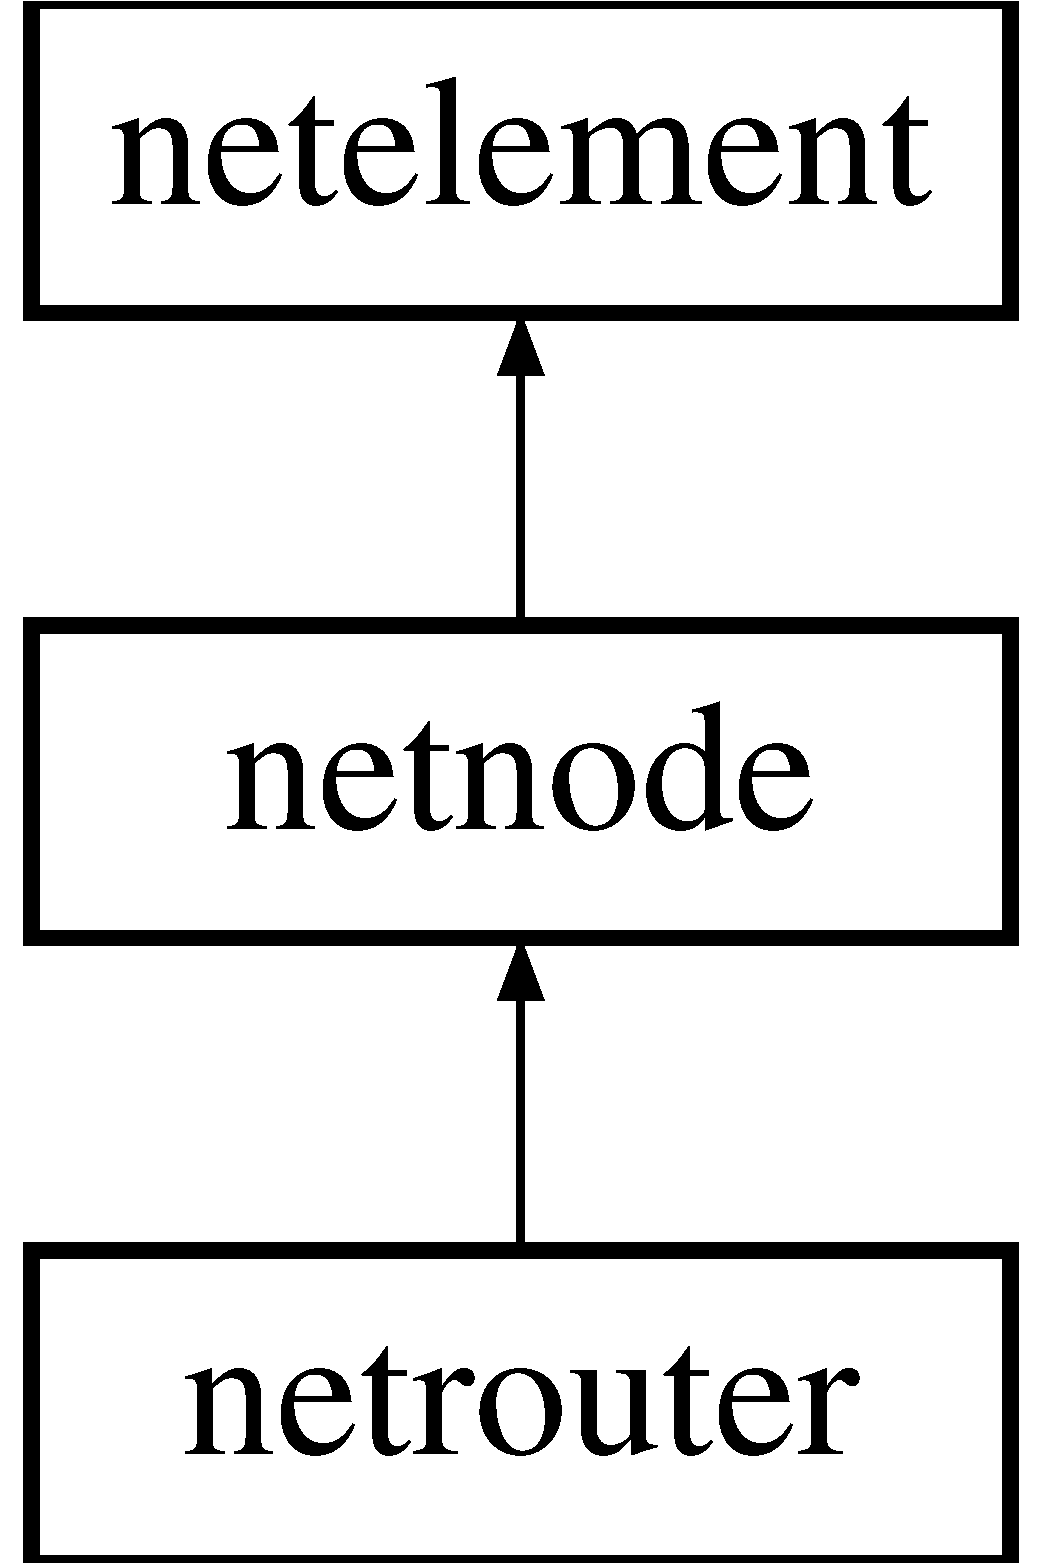
\includegraphics[height=3.000000cm]{classnetrouter}
\end{center}
\end{figure}
\subsection*{Public Member Functions}
\begin{DoxyCompactItemize}
\item 
\hyperlink{classnetrouter_a8ab7ff9ad09156e92ce58f229e158ce8}{netrouter} ()
\begin{DoxyCompactList}\small\item\em Default constructor. \end{DoxyCompactList}\item 
\hyperlink{classnetrouter_aa489048e7f69c270c509033ad1987d2f}{netrouter} (string name)
\begin{DoxyCompactList}\small\item\em Sets name to the given one and nesting depth to 0. \end{DoxyCompactList}\item 
\hyperlink{classnetrouter_ab0da794c63d0b3e7a5335670eab80098}{netrouter} (string name, vector$<$ \hyperlink{classnetlink}{netlink} $\ast$ $>$ \hyperlink{classnetnode_af481c4109393b79170f523ca92bea507}{links})
\begin{DoxyCompactList}\small\item\em Sets name to the given one and the list of links attached to this router to the given one. \end{DoxyCompactList}\item 
virtual bool \hyperlink{classnetrouter_a1fa1b2262b7427485b31b2d90477b6e7}{is\-Routing\-Node} () const 
\begin{DoxyCompactList}\small\item\em Returns true, since this is a router. \end{DoxyCompactList}\item 
map$<$ \hyperlink{classnetlink}{netlink} $\ast$, \hyperlink{classpacket}{packet} $>$ \hyperlink{classnetrouter_a997f1c4c9951bc1a8323896db58a22ea}{receive\-Packet} (double time, \hyperlink{classsimulation}{simulation} \&sim, \hyperlink{classnetflow}{netflow} \&flow, \hyperlink{classpacket}{packet} \&pkt)
\begin{DoxyCompactList}\small\item\em This function forwards it along the best link for it to get to its destination as determined by the routing table. \end{DoxyCompactList}\item 
void \hyperlink{classnetrouter_af6e40bf81506f250c6f638df89cdb1c2}{receive\-Routing\-Packet} (double time, \hyperlink{classsimulation}{simulation} \&sim, \hyperlink{classpacket}{packet} \&pkt, \hyperlink{classnetlink}{netlink} \&link)
\begin{DoxyCompactList}\small\item\em If this is a R\-O\-U\-T\-I\-N\-G packet, this function will update the router's routing table and distances table if necessary. \end{DoxyCompactList}\item 
map$<$ string, double $>$ \hyperlink{classnetrouter_a58bea34e24bde952a64af47713be636f}{get\-R\-Distances} () const 
\begin{DoxyCompactList}\small\item\em Getter for the node distances collection. \end{DoxyCompactList}\item 
void \hyperlink{classnetrouter_a1a5540f9e742b6d4938401bfa54a2d02}{initialize\-Tables} (map$<$ string, \hyperlink{classnethost}{nethost} $\ast$ $>$ host\-\_\-list, map$<$ string, \hyperlink{classnetrouter}{netrouter} $\ast$ $>$ router\-\_\-list)
\begin{DoxyCompactList}\small\item\em Called once at the beginning of the simulation, after parsing in an input file. \end{DoxyCompactList}\item 
void \hyperlink{classnetrouter_a87c029bb86c80acc8a5c2878835ef5a1}{reset\-Distances} (map$<$ string, \hyperlink{classnethost}{nethost} $\ast$ $>$ host\-\_\-list, map$<$ string, \hyperlink{classnetrouter}{netrouter} $\ast$ $>$ router\-\_\-list)
\begin{DoxyCompactList}\small\item\em Called from each \hyperlink{classrouter__discovery__event}{router\-\_\-discovery\-\_\-event} before recalculating distances. \end{DoxyCompactList}\item 
virtual void \hyperlink{classnetrouter_abdb4669cfddd028629f6abedc38a9427}{print\-Helper} (ostream \&os) const 
\begin{DoxyCompactList}\small\item\em Print helper function which partially overrides the one in {\ttfamily netdevice}. \end{DoxyCompactList}\end{DoxyCompactItemize}
\subsection*{Additional Inherited Members}


\subsection{Detailed Description}
Represents a router in a simple network. 

The main difference from a {\ttfamily netnode} is that this object contains a routing table and a collection of distances to other nodes which is used to update the routing table. 

\subsection{Constructor \& Destructor Documentation}
\hypertarget{classnetrouter_a8ab7ff9ad09156e92ce58f229e158ce8}{\index{netrouter@{netrouter}!netrouter@{netrouter}}
\index{netrouter@{netrouter}!netrouter@{netrouter}}
\subsubsection[{netrouter}]{\setlength{\rightskip}{0pt plus 5cm}netrouter\-::netrouter (
\begin{DoxyParamCaption}
{}
\end{DoxyParamCaption}
)}}\label{classnetrouter_a8ab7ff9ad09156e92ce58f229e158ce8}


Default constructor. 

Sets name to empty string and nesting depth to 0. \hypertarget{classnetrouter_aa489048e7f69c270c509033ad1987d2f}{\index{netrouter@{netrouter}!netrouter@{netrouter}}
\index{netrouter@{netrouter}!netrouter@{netrouter}}
\subsubsection[{netrouter}]{\setlength{\rightskip}{0pt plus 5cm}netrouter\-::netrouter (
\begin{DoxyParamCaption}
\item[{string}]{name}
\end{DoxyParamCaption}
)}}\label{classnetrouter_aa489048e7f69c270c509033ad1987d2f}


Sets name to the given one and nesting depth to 0. 


\begin{DoxyParams}{Parameters}
{\em name} & of this router \\
\hline
\end{DoxyParams}
\hypertarget{classnetrouter_ab0da794c63d0b3e7a5335670eab80098}{\index{netrouter@{netrouter}!netrouter@{netrouter}}
\index{netrouter@{netrouter}!netrouter@{netrouter}}
\subsubsection[{netrouter}]{\setlength{\rightskip}{0pt plus 5cm}netrouter\-::netrouter (
\begin{DoxyParamCaption}
\item[{string}]{name, }
\item[{vector$<$ {\bf netlink} $\ast$ $>$}]{links}
\end{DoxyParamCaption}
)}}\label{classnetrouter_ab0da794c63d0b3e7a5335670eab80098}


Sets name to the given one and the list of links attached to this router to the given one. 


\begin{DoxyParams}{Parameters}
{\em name} & of this router \\
\hline
{\em links} & list of pointers to links attached to this router to copy into this object's list of link pointers \\
\hline
\end{DoxyParams}


\subsection{Member Function Documentation}
\hypertarget{classnetrouter_a58bea34e24bde952a64af47713be636f}{\index{netrouter@{netrouter}!get\-R\-Distances@{get\-R\-Distances}}
\index{get\-R\-Distances@{get\-R\-Distances}!netrouter@{netrouter}}
\subsubsection[{get\-R\-Distances}]{\setlength{\rightskip}{0pt plus 5cm}map$<$ string, double $>$ netrouter\-::get\-R\-Distances (
\begin{DoxyParamCaption}
{}
\end{DoxyParamCaption}
) const}}\label{classnetrouter_a58bea34e24bde952a64af47713be636f}


Getter for the node distances collection. 

\begin{DoxyReturn}{Returns}
collection of the distances of this router from all other nodes 
\end{DoxyReturn}
\hypertarget{classnetrouter_a1a5540f9e742b6d4938401bfa54a2d02}{\index{netrouter@{netrouter}!initialize\-Tables@{initialize\-Tables}}
\index{initialize\-Tables@{initialize\-Tables}!netrouter@{netrouter}}
\subsubsection[{initialize\-Tables}]{\setlength{\rightskip}{0pt plus 5cm}void netrouter\-::initialize\-Tables (
\begin{DoxyParamCaption}
\item[{map$<$ string, {\bf nethost} $\ast$ $>$}]{host\-\_\-list, }
\item[{map$<$ string, {\bf netrouter} $\ast$ $>$}]{router\-\_\-list}
\end{DoxyParamCaption}
)}}\label{classnetrouter_a1a5540f9e742b6d4938401bfa54a2d02}


Called once at the beginning of the simulation, after parsing in an input file. 

Sets distance to self and adjacent hosts to 0. Sets the correct link to adjacent hosts since each host has only one outgoing link. Sets other links to N\-U\-L\-L.


\begin{DoxyParams}{Parameters}
{\em host\-\_\-list} & list of all hosts \\
\hline
{\em router\-\_\-list} & list of all routers \\
\hline
\end{DoxyParams}
\hypertarget{classnetrouter_a1fa1b2262b7427485b31b2d90477b6e7}{\index{netrouter@{netrouter}!is\-Routing\-Node@{is\-Routing\-Node}}
\index{is\-Routing\-Node@{is\-Routing\-Node}!netrouter@{netrouter}}
\subsubsection[{is\-Routing\-Node}]{\setlength{\rightskip}{0pt plus 5cm}bool netrouter\-::is\-Routing\-Node (
\begin{DoxyParamCaption}
{}
\end{DoxyParamCaption}
) const\hspace{0.3cm}{\ttfamily [virtual]}}}\label{classnetrouter_a1fa1b2262b7427485b31b2d90477b6e7}


Returns true, since this is a router. 

\begin{DoxyReturn}{Returns}
true 
\end{DoxyReturn}


Implements \hyperlink{classnetnode_a4a8b5169af7145506be0d31f6307908a}{netnode}.

\hypertarget{classnetrouter_abdb4669cfddd028629f6abedc38a9427}{\index{netrouter@{netrouter}!print\-Helper@{print\-Helper}}
\index{print\-Helper@{print\-Helper}!netrouter@{netrouter}}
\subsubsection[{print\-Helper}]{\setlength{\rightskip}{0pt plus 5cm}void netrouter\-::print\-Helper (
\begin{DoxyParamCaption}
\item[{ostream \&}]{os}
\end{DoxyParamCaption}
) const\hspace{0.3cm}{\ttfamily [virtual]}}}\label{classnetrouter_abdb4669cfddd028629f6abedc38a9427}


Print helper function which partially overrides the one in {\ttfamily netdevice}. 


\begin{DoxyParams}{Parameters}
{\em os} & The output stream to which to write. \\
\hline
\end{DoxyParams}
\hypertarget{classnetrouter_a997f1c4c9951bc1a8323896db58a22ea}{\index{netrouter@{netrouter}!receive\-Packet@{receive\-Packet}}
\index{receive\-Packet@{receive\-Packet}!netrouter@{netrouter}}
\subsubsection[{receive\-Packet}]{\setlength{\rightskip}{0pt plus 5cm}map$<$ {\bf netlink} $\ast$, {\bf packet} $>$ netrouter\-::receive\-Packet (
\begin{DoxyParamCaption}
\item[{double}]{time, }
\item[{{\bf simulation} \&}]{sim, }
\item[{{\bf netflow} \&}]{flow, }
\item[{{\bf packet} \&}]{pkt}
\end{DoxyParamCaption}
)}}\label{classnetrouter_a997f1c4c9951bc1a8323896db58a22ea}


This function forwards it along the best link for it to get to its destination as determined by the routing table. 

Note that it's the caller's responsibility to generate the actual send\-\_\-packet\-\_\-events based on the returned map. 
\begin{DoxyParams}{Parameters}
{\em time} & of packet receipt \\
\hline
{\em sim} & \\
\hline
{\em flow} & parent flow, N\-U\-L\-L if R\-O\-U\-T\-I\-N\-G type \\
\hline
{\em pkt} & the arriving packet \\
\hline
\end{DoxyParams}
\begin{DoxyReturn}{Returns}
a map from the links to use to the corresponding packets 
\end{DoxyReturn}
\begin{DoxyWarning}{Warning}
deprecated for use with R\-O\-U\-T\-I\-N\-G packets! Use {\ttfamily receive\-Routing\-Packet} instead. 
\end{DoxyWarning}
\hypertarget{classnetrouter_af6e40bf81506f250c6f638df89cdb1c2}{\index{netrouter@{netrouter}!receive\-Routing\-Packet@{receive\-Routing\-Packet}}
\index{receive\-Routing\-Packet@{receive\-Routing\-Packet}!netrouter@{netrouter}}
\subsubsection[{receive\-Routing\-Packet}]{\setlength{\rightskip}{0pt plus 5cm}void netrouter\-::receive\-Routing\-Packet (
\begin{DoxyParamCaption}
\item[{double}]{time, }
\item[{{\bf simulation} \&}]{sim, }
\item[{{\bf packet} \&}]{pkt, }
\item[{{\bf netlink} \&}]{link}
\end{DoxyParamCaption}
)}}\label{classnetrouter_af6e40bf81506f250c6f638df89cdb1c2}


If this is a R\-O\-U\-T\-I\-N\-G packet, this function will update the router's routing table and distances table if necessary. 

If an update is made, it will also trigger send\-\_\-packet\-\_\-events to deliver additional routing packets to its neighbors. 
\begin{DoxyParams}{Parameters}
{\em time} & of receipt of trigger packet \\
\hline
{\em sim} & \\
\hline
{\em pkt} & received \\
\hline
{\em link} & it was received on \\
\hline
\end{DoxyParams}
\hypertarget{classnetrouter_a87c029bb86c80acc8a5c2878835ef5a1}{\index{netrouter@{netrouter}!reset\-Distances@{reset\-Distances}}
\index{reset\-Distances@{reset\-Distances}!netrouter@{netrouter}}
\subsubsection[{reset\-Distances}]{\setlength{\rightskip}{0pt plus 5cm}void netrouter\-::reset\-Distances (
\begin{DoxyParamCaption}
\item[{map$<$ string, {\bf nethost} $\ast$ $>$}]{host\-\_\-list, }
\item[{map$<$ string, {\bf netrouter} $\ast$ $>$}]{router\-\_\-list}
\end{DoxyParamCaption}
)}}\label{classnetrouter_a87c029bb86c80acc8a5c2878835ef5a1}


Called from each \hyperlink{classrouter__discovery__event}{router\-\_\-discovery\-\_\-event} before recalculating distances. 

Sets distances to all other routers and nonadjacent hosts to infinity. 
\begin{DoxyParams}{Parameters}
{\em host\-\_\-list} & list of all hosts \\
\hline
{\em router\-\_\-list} & list of all routers \\
\hline
\end{DoxyParams}


The documentation for this class was generated from the following files\-:\begin{DoxyCompactItemize}
\item 
src/\hyperlink{network_8h}{network.\-h}\item 
src/network.\-cpp\end{DoxyCompactItemize}

\hypertarget{classpacket}{\section{packet Class Reference}
\label{classpacket}\index{packet@{packet}}
}


Describes a packet in the simulated network, which can be one of the types in the enumerated type {\ttfamily packet\-Type}.  




{\ttfamily \#include $<$network.\-h$>$}

Inheritance diagram for packet\-:\begin{figure}[H]
\begin{center}
\leavevmode
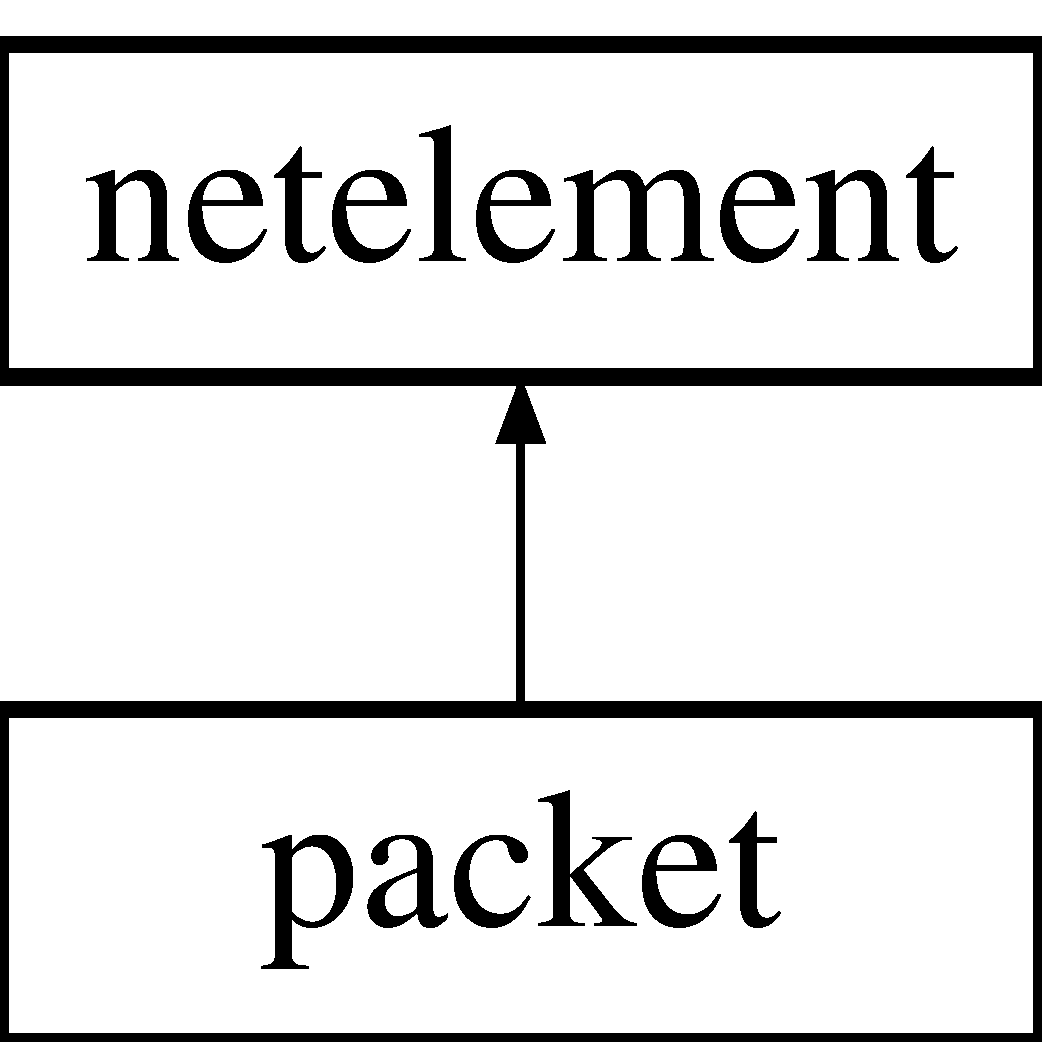
\includegraphics[height=2.000000cm]{classpacket}
\end{center}
\end{figure}
\subsection*{Public Member Functions}
\begin{DoxyCompactItemize}
\item 
\hyperlink{classpacket_ae33ebc35602983d12aa139f050f77938}{packet} ()
\begin{DoxyCompactList}\small\item\em Default contructor. \end{DoxyCompactList}\item 
\hyperlink{classpacket_ae65d1c323eff4f7bc1c092d42b52fd30}{packet} (\hyperlink{util_8h_ad875bcb78f9bd8625c5e454cafdc8de7}{packet\-\_\-type} type, const string \&source\-\_\-ip, const string \&dest\-\_\-ip)
\begin{DoxyCompactList}\small\item\em This constructor infers the size of a packet from the given type, which must be R\-O\-U\-T\-I\-N\-G since there's no parent flow and no sequence number. \end{DoxyCompactList}\item 
\hyperlink{classpacket_a32d7fad8b9fb8e6b130d6d93fefb675d}{packet} (\hyperlink{util_8h_ad875bcb78f9bd8625c5e454cafdc8de7}{packet\-\_\-type} type, \hyperlink{classnetflow}{netflow} \&parent\-\_\-flow, int seqnum)
\begin{DoxyCompactList}\small\item\em This constructor infers the size of a packet from the given type, which must be A\-C\-K or F\-L\-O\-W since the source and destination are inferred from a parent flow. \end{DoxyCompactList}\item 
bool \hyperlink{classpacket_ae85fc39129ba8cc568a56d2b5f7dfa29}{is\-Null\-Packet} () const 
\begin{DoxyCompactList}\small\item\em Some functions are forced to return a packet value, so the default packet constructor makes packets with ids of 0, and they're considered null in calling functions. \end{DoxyCompactList}\item 
string \hyperlink{classpacket_a9df0e590a6e0528a44f5109059e67e87}{get\-Source} () const 
\begin{DoxyCompactList}\small\item\em Getter for the source host of this packet. \end{DoxyCompactList}\item 
string \hyperlink{classpacket_a1b2e0681850de65dd7cf384a0ac62b36}{get\-Destination} () const 
\begin{DoxyCompactList}\small\item\em Getter for the destination host of this packet. \end{DoxyCompactList}\item 
int \hyperlink{classpacket_a73ded904b5e293e7e33ae1a57d470fd5}{get\-Seq} () const 
\begin{DoxyCompactList}\small\item\em Getter for the sequence number of this packet. \end{DoxyCompactList}\item 
long \hyperlink{classpacket_a6bd880d868f03dd6ac2ef29053e6612d}{get\-Id} () const 
\begin{DoxyCompactList}\small\item\em Getter for the unique I\-D of this packet. \end{DoxyCompactList}\item 
const map$<$ string, double $>$ \& \hyperlink{classpacket_a65ccf9c5fd0833c0070b62204268d533}{get\-Distances} () const 
\begin{DoxyCompactList}\small\item\em Getter for the distances map. \end{DoxyCompactList}\item 
void \hyperlink{classpacket_a989bc3f928b4254b6130e286bff83db6}{set\-Distances} (map$<$ string, double $>$ distances)
\begin{DoxyCompactList}\small\item\em Setter for the distances map. \end{DoxyCompactList}\item 
\hyperlink{classnetflow}{netflow} $\ast$ \hyperlink{classpacket_aa6a8a41c8147772a01a97c1100b9ed11}{get\-Parent\-Flow} () const 
\begin{DoxyCompactList}\small\item\em Getter for the parent flow of this packet. \end{DoxyCompactList}\item 
\hyperlink{util_8h_ad875bcb78f9bd8625c5e454cafdc8de7}{packet\-\_\-type} \hyperlink{classpacket_ae71a8e7630d96485dac3b2a68371caff}{get\-Type} () const 
\begin{DoxyCompactList}\small\item\em Getter for the type of this packet. \end{DoxyCompactList}\item 
double \hyperlink{classpacket_a58e64ca03f52a042dca4268c608ca6b2}{get\-Size\-Mb} () const 
\begin{DoxyCompactList}\small\item\em Getter for the size in megabits of this packet. \end{DoxyCompactList}\item 
long \hyperlink{classpacket_a936359db71dc4a210e5b53d614cf3b79}{get\-Size\-Bytes} () const 
\begin{DoxyCompactList}\small\item\em Getter for the size in bytes of this packet. \end{DoxyCompactList}\item 
string \hyperlink{classpacket_ac5c6ad2cc857a2c93def278a6cb37829}{get\-Type\-String} () const 
\begin{DoxyCompactList}\small\item\em Getter for the type of this packet as a string. \end{DoxyCompactList}\item 
double \hyperlink{classpacket_a6deed8840b2e675824633f123b07734b}{get\-Transmit\-Timestamp} () const 
\begin{DoxyCompactList}\small\item\em Getter for the transmit timestamp for this packet. \end{DoxyCompactList}\item 
void \hyperlink{classpacket_ad9cf233e7dc54745944934d1aa9adf51}{set\-Transmit\-Timestamp} (double time)
\begin{DoxyCompactList}\small\item\em Setter for the transmit timestamp. \end{DoxyCompactList}\item 
virtual void \hyperlink{classpacket_a5f0d34c38a7f075a99cf701c6e9ee5bf}{print\-Helper} (ostream \&os) const 
\begin{DoxyCompactList}\small\item\em Print helper function which partially overrides the one in {\ttfamily netdevice}. \end{DoxyCompactList}\end{DoxyCompactItemize}
\subsection*{Static Public Attributes}
\begin{DoxyCompactItemize}
\item 
static long \hyperlink{classpacket_adc3b99f39d577549ea3701d4b4de2839}{id\-\_\-gen} = 1
\begin{DoxyCompactList}\small\item\em Unique I\-D number generator. \end{DoxyCompactList}\end{DoxyCompactItemize}


\subsection{Detailed Description}
Describes a packet in the simulated network, which can be one of the types in the enumerated type {\ttfamily packet\-Type}. 

Note that a real packet would have a payload but this class doesn't provide for one. 

\subsection{Constructor \& Destructor Documentation}
\hypertarget{classpacket_ae33ebc35602983d12aa139f050f77938}{\index{packet@{packet}!packet@{packet}}
\index{packet@{packet}!packet@{packet}}
\subsubsection[{packet}]{\setlength{\rightskip}{0pt plus 5cm}packet\-::packet (
\begin{DoxyParamCaption}
{}
\end{DoxyParamCaption}
)}}\label{classpacket_ae33ebc35602983d12aa139f050f77938}


Default contructor. 

Sets everything to dummy values. \hypertarget{classpacket_ae65d1c323eff4f7bc1c092d42b52fd30}{\index{packet@{packet}!packet@{packet}}
\index{packet@{packet}!packet@{packet}}
\subsubsection[{packet}]{\setlength{\rightskip}{0pt plus 5cm}packet\-::packet (
\begin{DoxyParamCaption}
\item[{{\bf packet\-\_\-type}}]{type, }
\item[{const string \&}]{source\-\_\-ip, }
\item[{const string \&}]{dest\-\_\-ip}
\end{DoxyParamCaption}
)}}\label{classpacket_ae65d1c323eff4f7bc1c092d42b52fd30}


This constructor infers the size of a packet from the given type, which must be R\-O\-U\-T\-I\-N\-G since there's no parent flow and no sequence number. 

and no sequence number.


\begin{DoxyParams}{Parameters}
{\em type} & one of the values of the {\ttfamily packet\-\_\-type} enum, but must be R\-O\-U\-T\-I\-N\-G for this constructor \\
\hline
{\em source\-\_\-ip} & the N\-A\-M\-E (since this simulation uses names, not I\-Ps) of the original source which must be a router \\
\hline
{\em dest\-\_\-ip} & the N\-A\-M\-E of the ultimate destination, which must be a router\\
\hline
\end{DoxyParams}
\begin{DoxyWarning}{Warning}
assertion triggered if the packet type isn't R\-O\-U\-T\-I\-N\-G 
\end{DoxyWarning}
\hypertarget{classpacket_a32d7fad8b9fb8e6b130d6d93fefb675d}{\index{packet@{packet}!packet@{packet}}
\index{packet@{packet}!packet@{packet}}
\subsubsection[{packet}]{\setlength{\rightskip}{0pt plus 5cm}packet\-::packet (
\begin{DoxyParamCaption}
\item[{{\bf packet\-\_\-type}}]{type, }
\item[{{\bf netflow} \&}]{parent\-\_\-flow, }
\item[{int}]{seqnum}
\end{DoxyParamCaption}
)}}\label{classpacket_a32d7fad8b9fb8e6b130d6d93fefb675d}


This constructor infers the size of a packet from the given type, which must be A\-C\-K or F\-L\-O\-W since the source and destination are inferred from a parent flow. 


\begin{DoxyParams}{Parameters}
{\em type} & one of the values of the {\ttfamily packet\-\_\-type} enum, but must be R\-O\-U\-T\-I\-N\-G for this constructor \\
\hline
{\em parent\-\_\-flow} & flow to which this packet belongs. A\-C\-K and F\-L\-O\-W packets belong to flows. \\
\hline
{\em seqnum} & sequence number for this packet, where the first packet in flow is numbered 1. Pass in anything (or {\ttfamily S\-E\-Q\-N\-U\-M\-\_\-\-F\-O\-R\-\_\-\-N\-O\-N\-F\-L\-O\-W\-S}) for A\-C\-K packets; their seqnums are just set to {\ttfamily S\-E\-Q\-N\-U\-M\-\_\-\-F\-O\-R\-\_\-\-N\-O\-N\-F\-L\-O\-W\-S}.\\
\hline
\end{DoxyParams}
\begin{DoxyWarning}{Warning}
assertion is triggered if the packet type is not A\-C\-K or F\-L\-O\-W. 
\end{DoxyWarning}


\subsection{Member Function Documentation}
\hypertarget{classpacket_a1b2e0681850de65dd7cf384a0ac62b36}{\index{packet@{packet}!get\-Destination@{get\-Destination}}
\index{get\-Destination@{get\-Destination}!packet@{packet}}
\subsubsection[{get\-Destination}]{\setlength{\rightskip}{0pt plus 5cm}string packet\-::get\-Destination (
\begin{DoxyParamCaption}
{}
\end{DoxyParamCaption}
) const}}\label{classpacket_a1b2e0681850de65dd7cf384a0ac62b36}


Getter for the destination host of this packet. 

\begin{DoxyReturn}{Returns}
destination host name 
\end{DoxyReturn}
\hypertarget{classpacket_a65ccf9c5fd0833c0070b62204268d533}{\index{packet@{packet}!get\-Distances@{get\-Distances}}
\index{get\-Distances@{get\-Distances}!packet@{packet}}
\subsubsection[{get\-Distances}]{\setlength{\rightskip}{0pt plus 5cm}const map$<$ string, double $>$ \& packet\-::get\-Distances (
\begin{DoxyParamCaption}
{}
\end{DoxyParamCaption}
) const}}\label{classpacket_a65ccf9c5fd0833c0070b62204268d533}


Getter for the distances map. 

\begin{DoxyReturn}{Returns}
distnaces map 
\end{DoxyReturn}
\hypertarget{classpacket_a6bd880d868f03dd6ac2ef29053e6612d}{\index{packet@{packet}!get\-Id@{get\-Id}}
\index{get\-Id@{get\-Id}!packet@{packet}}
\subsubsection[{get\-Id}]{\setlength{\rightskip}{0pt plus 5cm}long packet\-::get\-Id (
\begin{DoxyParamCaption}
{}
\end{DoxyParamCaption}
) const}}\label{classpacket_a6bd880d868f03dd6ac2ef29053e6612d}


Getter for the unique I\-D of this packet. 

\begin{DoxyReturn}{Returns}
I\-D number 
\end{DoxyReturn}
\hypertarget{classpacket_aa6a8a41c8147772a01a97c1100b9ed11}{\index{packet@{packet}!get\-Parent\-Flow@{get\-Parent\-Flow}}
\index{get\-Parent\-Flow@{get\-Parent\-Flow}!packet@{packet}}
\subsubsection[{get\-Parent\-Flow}]{\setlength{\rightskip}{0pt plus 5cm}{\bf netflow} $\ast$ packet\-::get\-Parent\-Flow (
\begin{DoxyParamCaption}
{}
\end{DoxyParamCaption}
) const}}\label{classpacket_aa6a8a41c8147772a01a97c1100b9ed11}


Getter for the parent flow of this packet. 

\begin{DoxyReturn}{Returns}
parent flow 
\end{DoxyReturn}
\hypertarget{classpacket_a73ded904b5e293e7e33ae1a57d470fd5}{\index{packet@{packet}!get\-Seq@{get\-Seq}}
\index{get\-Seq@{get\-Seq}!packet@{packet}}
\subsubsection[{get\-Seq}]{\setlength{\rightskip}{0pt plus 5cm}int packet\-::get\-Seq (
\begin{DoxyParamCaption}
{}
\end{DoxyParamCaption}
) const}}\label{classpacket_a73ded904b5e293e7e33ae1a57d470fd5}


Getter for the sequence number of this packet. 

\begin{DoxyReturn}{Returns}
sequence number 
\end{DoxyReturn}
\hypertarget{classpacket_a936359db71dc4a210e5b53d614cf3b79}{\index{packet@{packet}!get\-Size\-Bytes@{get\-Size\-Bytes}}
\index{get\-Size\-Bytes@{get\-Size\-Bytes}!packet@{packet}}
\subsubsection[{get\-Size\-Bytes}]{\setlength{\rightskip}{0pt plus 5cm}long packet\-::get\-Size\-Bytes (
\begin{DoxyParamCaption}
{}
\end{DoxyParamCaption}
) const}}\label{classpacket_a936359db71dc4a210e5b53d614cf3b79}


Getter for the size in bytes of this packet. 

\begin{DoxyReturn}{Returns}
size in bytes. 
\end{DoxyReturn}
\hypertarget{classpacket_a58e64ca03f52a042dca4268c608ca6b2}{\index{packet@{packet}!get\-Size\-Mb@{get\-Size\-Mb}}
\index{get\-Size\-Mb@{get\-Size\-Mb}!packet@{packet}}
\subsubsection[{get\-Size\-Mb}]{\setlength{\rightskip}{0pt plus 5cm}double packet\-::get\-Size\-Mb (
\begin{DoxyParamCaption}
{}
\end{DoxyParamCaption}
) const}}\label{classpacket_a58e64ca03f52a042dca4268c608ca6b2}


Getter for the size in megabits of this packet. 

\begin{DoxyReturn}{Returns}
size in megabits. 
\end{DoxyReturn}
\hypertarget{classpacket_a9df0e590a6e0528a44f5109059e67e87}{\index{packet@{packet}!get\-Source@{get\-Source}}
\index{get\-Source@{get\-Source}!packet@{packet}}
\subsubsection[{get\-Source}]{\setlength{\rightskip}{0pt plus 5cm}string packet\-::get\-Source (
\begin{DoxyParamCaption}
{}
\end{DoxyParamCaption}
) const}}\label{classpacket_a9df0e590a6e0528a44f5109059e67e87}


Getter for the source host of this packet. 

\begin{DoxyReturn}{Returns}
source host name 
\end{DoxyReturn}
\hypertarget{classpacket_a6deed8840b2e675824633f123b07734b}{\index{packet@{packet}!get\-Transmit\-Timestamp@{get\-Transmit\-Timestamp}}
\index{get\-Transmit\-Timestamp@{get\-Transmit\-Timestamp}!packet@{packet}}
\subsubsection[{get\-Transmit\-Timestamp}]{\setlength{\rightskip}{0pt plus 5cm}double packet\-::get\-Transmit\-Timestamp (
\begin{DoxyParamCaption}
{}
\end{DoxyParamCaption}
) const}}\label{classpacket_a6deed8840b2e675824633f123b07734b}


Getter for the transmit timestamp for this packet. 

\begin{DoxyReturn}{Returns}
transmit timestamp 
\end{DoxyReturn}
\hypertarget{classpacket_ae71a8e7630d96485dac3b2a68371caff}{\index{packet@{packet}!get\-Type@{get\-Type}}
\index{get\-Type@{get\-Type}!packet@{packet}}
\subsubsection[{get\-Type}]{\setlength{\rightskip}{0pt plus 5cm}{\bf packet\-\_\-type} packet\-::get\-Type (
\begin{DoxyParamCaption}
{}
\end{DoxyParamCaption}
) const}}\label{classpacket_ae71a8e7630d96485dac3b2a68371caff}


Getter for the type of this packet. 

\begin{DoxyReturn}{Returns}
packet type 
\end{DoxyReturn}
\hypertarget{classpacket_ac5c6ad2cc857a2c93def278a6cb37829}{\index{packet@{packet}!get\-Type\-String@{get\-Type\-String}}
\index{get\-Type\-String@{get\-Type\-String}!packet@{packet}}
\subsubsection[{get\-Type\-String}]{\setlength{\rightskip}{0pt plus 5cm}string packet\-::get\-Type\-String (
\begin{DoxyParamCaption}
{}
\end{DoxyParamCaption}
) const}}\label{classpacket_ac5c6ad2cc857a2c93def278a6cb37829}


Getter for the type of this packet as a string. 

\begin{DoxyReturn}{Returns}
type as a string. 
\end{DoxyReturn}
\hypertarget{classpacket_ae85fc39129ba8cc568a56d2b5f7dfa29}{\index{packet@{packet}!is\-Null\-Packet@{is\-Null\-Packet}}
\index{is\-Null\-Packet@{is\-Null\-Packet}!packet@{packet}}
\subsubsection[{is\-Null\-Packet}]{\setlength{\rightskip}{0pt plus 5cm}bool packet\-::is\-Null\-Packet (
\begin{DoxyParamCaption}
{}
\end{DoxyParamCaption}
) const}}\label{classpacket_ae85fc39129ba8cc568a56d2b5f7dfa29}


Some functions are forced to return a packet value, so the default packet constructor makes packets with ids of 0, and they're considered null in calling functions. 

This function just checks if a given packet is a \char`\"{}fake\char`\"{} packet.

\begin{DoxyReturn}{Returns}
true if null packets 
\end{DoxyReturn}
\hypertarget{classpacket_a5f0d34c38a7f075a99cf701c6e9ee5bf}{\index{packet@{packet}!print\-Helper@{print\-Helper}}
\index{print\-Helper@{print\-Helper}!packet@{packet}}
\subsubsection[{print\-Helper}]{\setlength{\rightskip}{0pt plus 5cm}void packet\-::print\-Helper (
\begin{DoxyParamCaption}
\item[{ostream \&}]{os}
\end{DoxyParamCaption}
) const\hspace{0.3cm}{\ttfamily [virtual]}}}\label{classpacket_a5f0d34c38a7f075a99cf701c6e9ee5bf}


Print helper function which partially overrides the one in {\ttfamily netdevice}. 


\begin{DoxyParams}{Parameters}
{\em os} & The output stream to which to write. \\
\hline
\end{DoxyParams}
\hypertarget{classpacket_a989bc3f928b4254b6130e286bff83db6}{\index{packet@{packet}!set\-Distances@{set\-Distances}}
\index{set\-Distances@{set\-Distances}!packet@{packet}}
\subsubsection[{set\-Distances}]{\setlength{\rightskip}{0pt plus 5cm}void packet\-::set\-Distances (
\begin{DoxyParamCaption}
\item[{map$<$ string, double $>$}]{distances}
\end{DoxyParamCaption}
)}}\label{classpacket_a989bc3f928b4254b6130e286bff83db6}


Setter for the distances map. 


\begin{DoxyParams}{Parameters}
{\em distances} & \\
\hline
\end{DoxyParams}
\hypertarget{classpacket_ad9cf233e7dc54745944934d1aa9adf51}{\index{packet@{packet}!set\-Transmit\-Timestamp@{set\-Transmit\-Timestamp}}
\index{set\-Transmit\-Timestamp@{set\-Transmit\-Timestamp}!packet@{packet}}
\subsubsection[{set\-Transmit\-Timestamp}]{\setlength{\rightskip}{0pt plus 5cm}void packet\-::set\-Transmit\-Timestamp (
\begin{DoxyParamCaption}
\item[{double}]{time}
\end{DoxyParamCaption}
)}}\label{classpacket_ad9cf233e7dc54745944934d1aa9adf51}


Setter for the transmit timestamp. 


\begin{DoxyParams}{Parameters}
{\em time} & \\
\hline
\end{DoxyParams}


\subsection{Member Data Documentation}
\hypertarget{classpacket_adc3b99f39d577549ea3701d4b4de2839}{\index{packet@{packet}!id\-\_\-gen@{id\-\_\-gen}}
\index{id\-\_\-gen@{id\-\_\-gen}!packet@{packet}}
\subsubsection[{id\-\_\-gen}]{\setlength{\rightskip}{0pt plus 5cm}long packet\-::id\-\_\-gen = 1\hspace{0.3cm}{\ttfamily [static]}}}\label{classpacket_adc3b99f39d577549ea3701d4b4de2839}


Unique I\-D number generator. 

Initialized in corresponding cpp file. 

The documentation for this class was generated from the following files\-:\begin{DoxyCompactItemize}
\item 
src/\hyperlink{network_8h}{network.\-h}\item 
src/network.\-cpp\end{DoxyCompactItemize}

\hypertarget{classreceive__packet__event}{\section{receive\-\_\-packet\-\_\-event Class Reference}
\label{classreceive__packet__event}\index{receive\-\_\-packet\-\_\-event@{receive\-\_\-packet\-\_\-event}}
}


Event that represents the arrival of a packet at either an intermediate node (router) or a final destination (host).  




{\ttfamily \#include $<$events.\-h$>$}

Inheritance diagram for receive\-\_\-packet\-\_\-event\-:\begin{figure}[H]
\begin{center}
\leavevmode
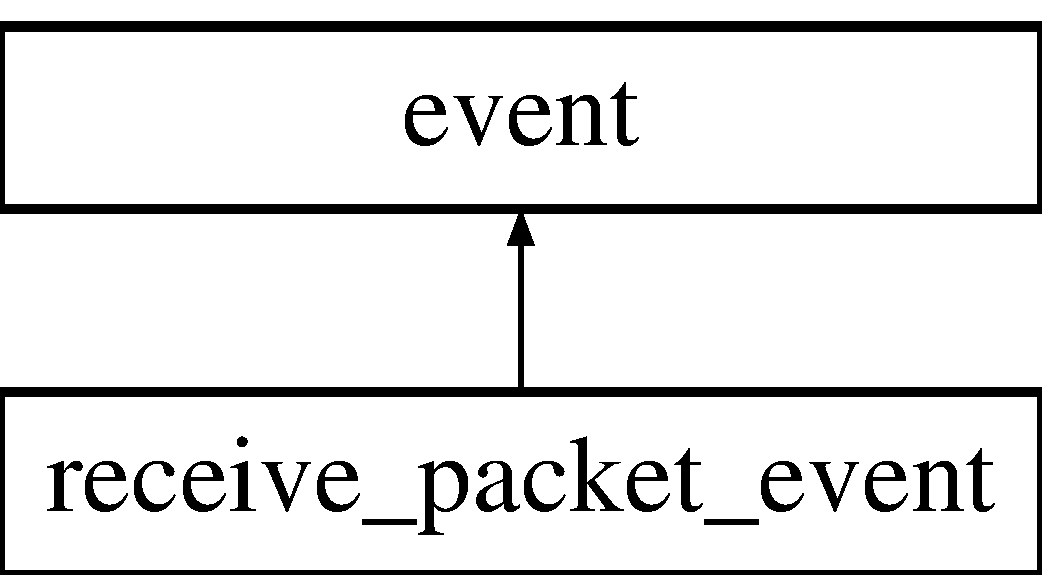
\includegraphics[height=2.000000cm]{classreceive__packet__event}
\end{center}
\end{figure}
\subsection*{Public Member Functions}
\begin{DoxyCompactItemize}
\item 
\hypertarget{classreceive__packet__event_ab160e0614169ef1ee78c52406a9dbcc4}{\hyperlink{classreceive__packet__event_ab160e0614169ef1ee78c52406a9dbcc4}{receive\-\_\-packet\-\_\-event} (double time, \hyperlink{classsimulation}{simulation} \&\hyperlink{classevent_a08c6d828bfb6f5539dcd1491e8ac77d2}{sim}, \hyperlink{classnetflow}{netflow} \&flow, \hyperlink{classpacket}{packet} \&pkt, \hyperlink{classnetnode}{netnode} \&step\-\_\-destination, \hyperlink{classnetlink}{netlink} \&link)}\label{classreceive__packet__event_ab160e0614169ef1ee78c52406a9dbcc4}

\begin{DoxyCompactList}\small\item\em Constructor for receive packet events for lone packets; the window size and start are set to 1 and this packet's sequence number, respectively. \end{DoxyCompactList}\item 
\hypertarget{classreceive__packet__event_a62cf5ad6dc6702e99182f297ad46f877}{\hyperlink{classreceive__packet__event_a62cf5ad6dc6702e99182f297ad46f877}{receive\-\_\-packet\-\_\-event} (double time, \hyperlink{classsimulation}{simulation} \&\hyperlink{classevent_a08c6d828bfb6f5539dcd1491e8ac77d2}{sim}, \hyperlink{classpacket}{packet} \&pkt, \hyperlink{classnetnode}{netnode} \&step\-\_\-destination, \hyperlink{classnetlink}{netlink} \&link)}\label{classreceive__packet__event_a62cf5ad6dc6702e99182f297ad46f877}

\begin{DoxyCompactList}\small\item\em Constructor for receive packet events for packets that do not belong to a flow (i.\-e., routing packets). \end{DoxyCompactList}\item 
\hyperlink{classreceive__packet__event_a5c41daa5c0cd069eb069b1a9cc450c65}{$\sim$receive\-\_\-packet\-\_\-event} ()
\begin{DoxyCompactList}\small\item\em Destructor. \end{DoxyCompactList}\item 
void \hyperlink{classreceive__packet__event_ae7c0b0f1defa3e225373bea73f98b2ba}{run\-Event} ()
\begin{DoxyCompactList}\small\item\em If this arrival event is at a router then we consult the routing table for the link to use for this packet's destination and use it to generate a \hyperlink{classsend__packet__event}{send\-\_\-packet\-\_\-event} down that link. \end{DoxyCompactList}\item 
void \hyperlink{classreceive__packet__event_a0da19ff9fc6f51c9599b095e064ee8ce}{print\-Helper} (ostream \&os)
\begin{DoxyCompactList}\small\item\em Print helper function. \end{DoxyCompactList}\end{DoxyCompactItemize}
\subsection*{Additional Inherited Members}


\subsection{Detailed Description}
Event that represents the arrival of a packet at either an intermediate node (router) or a final destination (host). 

The packet can be a F\-L\-O\-W, A\-C\-K, or R\-O\-U\-T\-I\-N\-G packet. 

\subsection{Constructor \& Destructor Documentation}
\hypertarget{classreceive__packet__event_a5c41daa5c0cd069eb069b1a9cc450c65}{\index{receive\-\_\-packet\-\_\-event@{receive\-\_\-packet\-\_\-event}!$\sim$receive\-\_\-packet\-\_\-event@{$\sim$receive\-\_\-packet\-\_\-event}}
\index{$\sim$receive\-\_\-packet\-\_\-event@{$\sim$receive\-\_\-packet\-\_\-event}!receive_packet_event@{receive\-\_\-packet\-\_\-event}}
\subsubsection[{$\sim$receive\-\_\-packet\-\_\-event}]{\setlength{\rightskip}{0pt plus 5cm}receive\-\_\-packet\-\_\-event\-::$\sim$receive\-\_\-packet\-\_\-event (
\begin{DoxyParamCaption}
{}
\end{DoxyParamCaption}
)}}\label{classreceive__packet__event_a5c41daa5c0cd069eb069b1a9cc450c65}


Destructor. 



\subsection{Member Function Documentation}
\hypertarget{classreceive__packet__event_a0da19ff9fc6f51c9599b095e064ee8ce}{\index{receive\-\_\-packet\-\_\-event@{receive\-\_\-packet\-\_\-event}!print\-Helper@{print\-Helper}}
\index{print\-Helper@{print\-Helper}!receive_packet_event@{receive\-\_\-packet\-\_\-event}}
\subsubsection[{print\-Helper}]{\setlength{\rightskip}{0pt plus 5cm}void receive\-\_\-packet\-\_\-event\-::print\-Helper (
\begin{DoxyParamCaption}
\item[{ostream \&}]{os}
\end{DoxyParamCaption}
)\hspace{0.3cm}{\ttfamily [virtual]}}}\label{classreceive__packet__event_a0da19ff9fc6f51c9599b095e064ee8ce}


Print helper function. 


\begin{DoxyParams}{Parameters}
{\em os} & The output stream to which to write event information. \\
\hline
\end{DoxyParams}


Reimplemented from \hyperlink{classevent_a14ef1b59ef1f5a8311c7cac315c271df}{event}.

\hypertarget{classreceive__packet__event_ae7c0b0f1defa3e225373bea73f98b2ba}{\index{receive\-\_\-packet\-\_\-event@{receive\-\_\-packet\-\_\-event}!run\-Event@{run\-Event}}
\index{run\-Event@{run\-Event}!receive_packet_event@{receive\-\_\-packet\-\_\-event}}
\subsubsection[{run\-Event}]{\setlength{\rightskip}{0pt plus 5cm}void receive\-\_\-packet\-\_\-event\-::run\-Event (
\begin{DoxyParamCaption}
{}
\end{DoxyParamCaption}
)\hspace{0.3cm}{\ttfamily [virtual]}}}\label{classreceive__packet__event_ae7c0b0f1defa3e225373bea73f98b2ba}


If this arrival event is at a router then we consult the routing table for the link to use for this packet's destination and use it to generate a \hyperlink{classsend__packet__event}{send\-\_\-packet\-\_\-event} down that link. 

If the packet is arriving at a host then we create an A\-C\-K packet, make and queue a \hyperlink{classsend__packet__event}{send\-\_\-packet\-\_\-event} for the A\-C\-K, and queue a future \hyperlink{classsend__packet__event}{send\-\_\-packet\-\_\-event} for a duplicate A\-C\-K in case we don't see the next packet in the sequence. We also remove the flow's pending duplicate A\-C\-K \hyperlink{classsend__packet__event}{send\-\_\-packet\-\_\-event} for the packet with the preceding sequence number. 

Reimplemented from \hyperlink{classevent_a74b7b9e3b4dd30fb42a2612968def7ef}{event}.



The documentation for this class was generated from the following files\-:\begin{DoxyCompactItemize}
\item 
src/\hyperlink{events_8h}{events.\-h}\item 
src/events.\-cpp\end{DoxyCompactItemize}

\hypertarget{classrouter__discovery__event}{\section{router\-\_\-discovery\-\_\-event Class Reference}
\label{classrouter__discovery__event}\index{router\-\_\-discovery\-\_\-event@{router\-\_\-discovery\-\_\-event}}
}


Event that triggers a given router's routing-\/table-\/population algorithm.  




{\ttfamily \#include $<$events.\-h$>$}

Inheritance diagram for router\-\_\-discovery\-\_\-event\-:\begin{figure}[H]
\begin{center}
\leavevmode
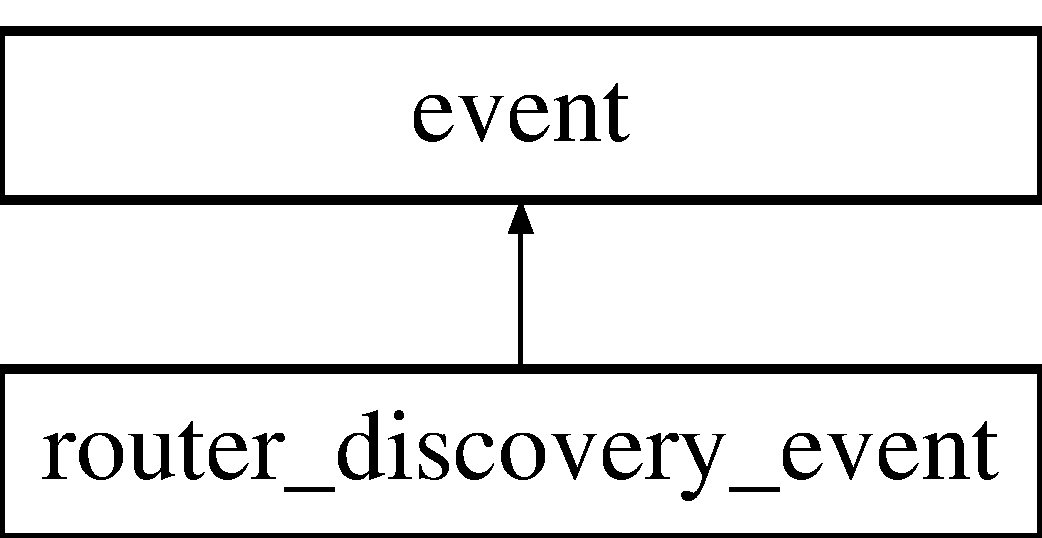
\includegraphics[height=2.000000cm]{classrouter__discovery__event}
\end{center}
\end{figure}
\subsection*{Public Member Functions}
\begin{DoxyCompactItemize}
\item 
\hypertarget{classrouter__discovery__event_af2a8465db9af4bde900f3bb1ccd8cde0}{\hyperlink{classrouter__discovery__event_af2a8465db9af4bde900f3bb1ccd8cde0}{router\-\_\-discovery\-\_\-event} (double time, \hyperlink{classsimulation}{simulation} \&\hyperlink{classevent_a08c6d828bfb6f5539dcd1491e8ac77d2}{sim})}\label{classrouter__discovery__event_af2a8465db9af4bde900f3bb1ccd8cde0}

\begin{DoxyCompactList}\small\item\em Initializes this event's time to the given one and sets the event I\-D,. \end{DoxyCompactList}\item 
\hypertarget{classrouter__discovery__event_a3c8b9beed6b979ee4240d1c0740b9488}{\hyperlink{classrouter__discovery__event_a3c8b9beed6b979ee4240d1c0740b9488}{$\sim$router\-\_\-discovery\-\_\-event} ()}\label{classrouter__discovery__event_a3c8b9beed6b979ee4240d1c0740b9488}

\begin{DoxyCompactList}\small\item\em Destructor. \end{DoxyCompactList}\item 
\hypertarget{classrouter__discovery__event_a170768272244ac6578a7c38ffd82733f}{void \hyperlink{classrouter__discovery__event_a170768272244ac6578a7c38ffd82733f}{run\-Event} ()}\label{classrouter__discovery__event_a170768272244ac6578a7c38ffd82733f}

\begin{DoxyCompactList}\small\item\em Runs the distributed Bellman-\/\-Ford algorithm from this router. \end{DoxyCompactList}\item 
void \hyperlink{classrouter__discovery__event_a32edb9914a54c925bbcb8a48d26451ed}{print\-Helper} (ostream \&os)
\begin{DoxyCompactList}\small\item\em Print helper function. \end{DoxyCompactList}\end{DoxyCompactItemize}
\subsection*{Additional Inherited Members}


\subsection{Detailed Description}
Event that triggers a given router's routing-\/table-\/population algorithm. 

\subsection{Member Function Documentation}
\hypertarget{classrouter__discovery__event_a32edb9914a54c925bbcb8a48d26451ed}{\index{router\-\_\-discovery\-\_\-event@{router\-\_\-discovery\-\_\-event}!print\-Helper@{print\-Helper}}
\index{print\-Helper@{print\-Helper}!router_discovery_event@{router\-\_\-discovery\-\_\-event}}
\subsubsection[{print\-Helper}]{\setlength{\rightskip}{0pt plus 5cm}void router\-\_\-discovery\-\_\-event\-::print\-Helper (
\begin{DoxyParamCaption}
\item[{ostream \&}]{os}
\end{DoxyParamCaption}
)\hspace{0.3cm}{\ttfamily [virtual]}}}\label{classrouter__discovery__event_a32edb9914a54c925bbcb8a48d26451ed}


Print helper function. 


\begin{DoxyParams}{Parameters}
{\em os} & The output stream to which to write event information. \\
\hline
\end{DoxyParams}


Reimplemented from \hyperlink{classevent_a14ef1b59ef1f5a8311c7cac315c271df}{event}.



The documentation for this class was generated from the following files\-:\begin{DoxyCompactItemize}
\item 
src/\hyperlink{events_8h}{events.\-h}\item 
src/events.\-cpp\end{DoxyCompactItemize}

\hypertarget{classsend__packet__event}{\section{send\-\_\-packet\-\_\-event Class Reference}
\label{classsend__packet__event}\index{send\-\_\-packet\-\_\-event@{send\-\_\-packet\-\_\-event}}
}


Sends a packet from a given departure node and down a given link whether it's an A\-C\-K, F\-L\-O\-W, or R\-O\-U\-T\-I\-N\-G packet.  




{\ttfamily \#include $<$events.\-h$>$}

Inheritance diagram for send\-\_\-packet\-\_\-event\-:\begin{figure}[H]
\begin{center}
\leavevmode
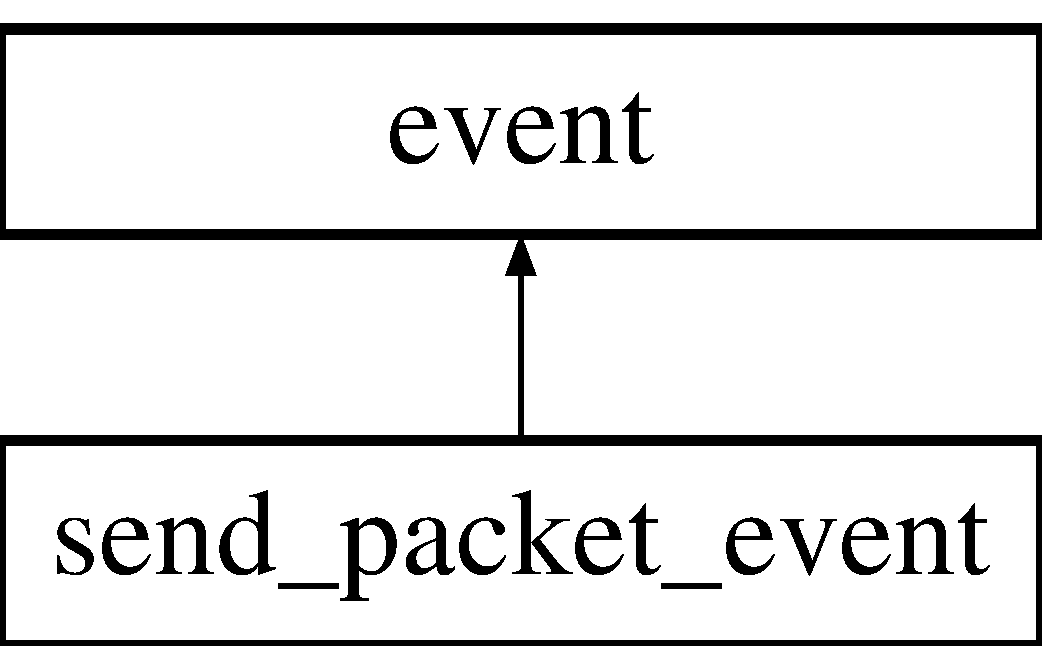
\includegraphics[height=2.000000cm]{classsend__packet__event}
\end{center}
\end{figure}
\subsection*{Public Member Functions}
\begin{DoxyCompactItemize}
\item 
\hyperlink{classsend__packet__event_a23728f781123d70f9499428c2fd61f58}{send\-\_\-packet\-\_\-event} ()
\begin{DoxyCompactList}\small\item\em Default constructor. \end{DoxyCompactList}\item 
\hyperlink{classsend__packet__event_a41388d80736ce35461e727fccf41d827}{send\-\_\-packet\-\_\-event} (double time, \hyperlink{classsimulation}{simulation} \&\hyperlink{classevent_a08c6d828bfb6f5539dcd1491e8ac77d2}{sim}, \hyperlink{classnetflow}{netflow} \&flow, \hyperlink{classpacket}{packet} \&pkt, \hyperlink{classnetlink}{netlink} \&link, \hyperlink{classnetnode}{netnode} \&departure\-\_\-node)
\begin{DoxyCompactList}\small\item\em Constructor for lone packets--window size is set to 1 and window\-\_\-start is set to this packet's sequence number. \end{DoxyCompactList}\item 
\hyperlink{classsend__packet__event_a38ce0bd431eae8069b627b44f55a4f2d}{send\-\_\-packet\-\_\-event} (double time, \hyperlink{classsimulation}{simulation} \&\hyperlink{classevent_a08c6d828bfb6f5539dcd1491e8ac77d2}{sim}, \hyperlink{classpacket}{packet} \&pkt, \hyperlink{classnetlink}{netlink} \&link, \hyperlink{classnetnode}{netnode} \&departure\-\_\-node)
\begin{DoxyCompactList}\small\item\em Constructor for packets that do not belong to a flow (i.\-e., routing packets). \end{DoxyCompactList}\item 
\hypertarget{classsend__packet__event_aab23e16e033bbf20a22ae74bb3709e12}{\hyperlink{classsend__packet__event_aab23e16e033bbf20a22ae74bb3709e12}{$\sim$send\-\_\-packet\-\_\-event} ()}\label{classsend__packet__event_aab23e16e033bbf20a22ae74bb3709e12}

\begin{DoxyCompactList}\small\item\em Destructor. \end{DoxyCompactList}\item 
void \hyperlink{classsend__packet__event_a844d3bf4a98011f4d128d05a8fb1a2db}{run\-Event} ()
\begin{DoxyCompactList}\small\item\em Finds time of arrival to next node from the given departure node down the given link and uses the arrival time to queue a \hyperlink{classreceive__packet__event}{receive\-\_\-packet\-\_\-event} (does nothing if the link buffer has no room, thereby dropping the packet). \end{DoxyCompactList}\item 
void \hyperlink{classsend__packet__event_a6f0f2911a15eef124ee57b1443a0b1d6}{print\-Helper} (ostream \&os)
\begin{DoxyCompactList}\small\item\em Print helper function. \end{DoxyCompactList}\end{DoxyCompactItemize}
\subsection*{Additional Inherited Members}


\subsection{Detailed Description}
Sends a packet from a given departure node and down a given link whether it's an A\-C\-K, F\-L\-O\-W, or R\-O\-U\-T\-I\-N\-G packet. 

Assumes that timeout\-\_\-events and other flow attributes like highest\-\_\-sent\-\_\-seqnum have been dealt with before this event runs. 

\subsection{Constructor \& Destructor Documentation}
\hypertarget{classsend__packet__event_a23728f781123d70f9499428c2fd61f58}{\index{send\-\_\-packet\-\_\-event@{send\-\_\-packet\-\_\-event}!send\-\_\-packet\-\_\-event@{send\-\_\-packet\-\_\-event}}
\index{send\-\_\-packet\-\_\-event@{send\-\_\-packet\-\_\-event}!send_packet_event@{send\-\_\-packet\-\_\-event}}
\subsubsection[{send\-\_\-packet\-\_\-event}]{\setlength{\rightskip}{0pt plus 5cm}send\-\_\-packet\-\_\-event\-::send\-\_\-packet\-\_\-event (
\begin{DoxyParamCaption}
{}
\end{DoxyParamCaption}
)}}\label{classsend__packet__event_a23728f781123d70f9499428c2fd61f58}


Default constructor. 

Sets everything to dummy or N\-U\-L\-L values. \hypertarget{classsend__packet__event_a41388d80736ce35461e727fccf41d827}{\index{send\-\_\-packet\-\_\-event@{send\-\_\-packet\-\_\-event}!send\-\_\-packet\-\_\-event@{send\-\_\-packet\-\_\-event}}
\index{send\-\_\-packet\-\_\-event@{send\-\_\-packet\-\_\-event}!send_packet_event@{send\-\_\-packet\-\_\-event}}
\subsubsection[{send\-\_\-packet\-\_\-event}]{\setlength{\rightskip}{0pt plus 5cm}send\-\_\-packet\-\_\-event\-::send\-\_\-packet\-\_\-event (
\begin{DoxyParamCaption}
\item[{double}]{time, }
\item[{{\bf simulation} \&}]{sim, }
\item[{{\bf netflow} \&}]{flow, }
\item[{{\bf packet} \&}]{pkt, }
\item[{{\bf netlink} \&}]{link, }
\item[{{\bf netnode} \&}]{departure\-\_\-node}
\end{DoxyParamCaption}
)}}\label{classsend__packet__event_a41388d80736ce35461e727fccf41d827}


Constructor for lone packets--window size is set to 1 and window\-\_\-start is set to this packet's sequence number. 


\begin{DoxyParams}{Parameters}
{\em time} & time at which to send the packet \\
\hline
{\em sim} & \\
\hline
{\em flow} & flow to which this packet belongs \\
\hline
{\em pkt} & packet to send \\
\hline
{\em link} & to send the packet on \\
\hline
{\em departure\-\_\-node} & node from which this packet will leave \\
\hline
\end{DoxyParams}
\hypertarget{classsend__packet__event_a38ce0bd431eae8069b627b44f55a4f2d}{\index{send\-\_\-packet\-\_\-event@{send\-\_\-packet\-\_\-event}!send\-\_\-packet\-\_\-event@{send\-\_\-packet\-\_\-event}}
\index{send\-\_\-packet\-\_\-event@{send\-\_\-packet\-\_\-event}!send_packet_event@{send\-\_\-packet\-\_\-event}}
\subsubsection[{send\-\_\-packet\-\_\-event}]{\setlength{\rightskip}{0pt plus 5cm}send\-\_\-packet\-\_\-event\-::send\-\_\-packet\-\_\-event (
\begin{DoxyParamCaption}
\item[{double}]{time, }
\item[{{\bf simulation} \&}]{sim, }
\item[{{\bf packet} \&}]{pkt, }
\item[{{\bf netlink} \&}]{link, }
\item[{{\bf netnode} \&}]{departure\-\_\-node}
\end{DoxyParamCaption}
)}}\label{classsend__packet__event_a38ce0bd431eae8069b627b44f55a4f2d}


Constructor for packets that do not belong to a flow (i.\-e., routing packets). 


\begin{DoxyParams}{Parameters}
{\em time} & time at which to send the packet \\
\hline
{\em sim} & \\
\hline
{\em pkt} & packet to send \\
\hline
{\em link} & to send the packet on \\
\hline
{\em departure\-\_\-node} & node from which this packet will leave \\
\hline
\end{DoxyParams}


\subsection{Member Function Documentation}
\hypertarget{classsend__packet__event_a6f0f2911a15eef124ee57b1443a0b1d6}{\index{send\-\_\-packet\-\_\-event@{send\-\_\-packet\-\_\-event}!print\-Helper@{print\-Helper}}
\index{print\-Helper@{print\-Helper}!send_packet_event@{send\-\_\-packet\-\_\-event}}
\subsubsection[{print\-Helper}]{\setlength{\rightskip}{0pt plus 5cm}void send\-\_\-packet\-\_\-event\-::print\-Helper (
\begin{DoxyParamCaption}
\item[{ostream \&}]{os}
\end{DoxyParamCaption}
)\hspace{0.3cm}{\ttfamily [virtual]}}}\label{classsend__packet__event_a6f0f2911a15eef124ee57b1443a0b1d6}


Print helper function. 


\begin{DoxyParams}{Parameters}
{\em os} & The output stream to which to write event information. \\
\hline
\end{DoxyParams}


Reimplemented from \hyperlink{classevent_a14ef1b59ef1f5a8311c7cac315c271df}{event}.

\hypertarget{classsend__packet__event_a844d3bf4a98011f4d128d05a8fb1a2db}{\index{send\-\_\-packet\-\_\-event@{send\-\_\-packet\-\_\-event}!run\-Event@{run\-Event}}
\index{run\-Event@{run\-Event}!send_packet_event@{send\-\_\-packet\-\_\-event}}
\subsubsection[{run\-Event}]{\setlength{\rightskip}{0pt plus 5cm}void send\-\_\-packet\-\_\-event\-::run\-Event (
\begin{DoxyParamCaption}
{}
\end{DoxyParamCaption}
)\hspace{0.3cm}{\ttfamily [virtual]}}}\label{classsend__packet__event_a844d3bf4a98011f4d128d05a8fb1a2db}


Finds time of arrival to next node from the given departure node down the given link and uses the arrival time to queue a \hyperlink{classreceive__packet__event}{receive\-\_\-packet\-\_\-event} (does nothing if the link buffer has no room, thereby dropping the packet). 

Doesn't make or queue timeout events because they should have been made and queued in parallel with the \hyperlink{classsend__packet__event}{send\-\_\-packet\-\_\-event}. 

Reimplemented from \hyperlink{classevent_a74b7b9e3b4dd30fb42a2612968def7ef}{event}.



The documentation for this class was generated from the following files\-:\begin{DoxyCompactItemize}
\item 
src/\hyperlink{events_8h}{events.\-h}\item 
src/events.\-cpp\end{DoxyCompactItemize}

\hypertarget{classsimulation}{\section{simulation Class Reference}
\label{classsimulation}\index{simulation@{simulation}}
}


Represents the simulation.  




{\ttfamily \#include $<$simulation.\-h$>$}

\subsection*{Public Member Functions}
\begin{DoxyCompactItemize}
\item 
\hyperlink{classsimulation_a4d5d5e617072409f1e5161ab048417df}{simulation} (const char $\ast$inputfile)
\begin{DoxyCompactList}\small\item\em Parses the J\-S\-O\-N file stored at {\ttfamily inputfile} and populates in-\/memory hosts, routers, links, and flows. \end{DoxyCompactList}\item 
\hyperlink{classsimulation_ae87d935230f2887512bbea182b0b5cda}{simulation} ()
\begin{DoxyCompactList}\small\item\em Default constructor which does nothing. \end{DoxyCompactList}\item 
\hypertarget{classsimulation_ac84df84c712163d5378db4b4fe62bc98}{\hyperlink{classsimulation_ac84df84c712163d5378db4b4fe62bc98}{$\sim$simulation} ()}\label{classsimulation_ac84df84c712163d5378db4b4fe62bc98}

\begin{DoxyCompactList}\small\item\em Deletes all the dynamically allocated network objects like hosts, routers, and so forth. \end{DoxyCompactList}\item 
void \hyperlink{classsimulation_ab9cca253149bda798b6eb13d1cf5638b}{parse\-\_\-\-J\-S\-O\-N\-\_\-input} (string jsonstring)
\begin{DoxyCompactList}\small\item\em Takes the full J\-S\-O\-N string passed in, parses it, and fills the in-\/memory collections of hosts, routers, links, and flows. \end{DoxyCompactList}\item 
void \hyperlink{classsimulation_a366ffcaf60b3a5eb1ff42f1524af2951}{print\-\_\-network} (ostream \&os) const 
\begin{DoxyCompactList}\small\item\em Prints hosts, routers, links, and flows to given output stream. \end{DoxyCompactList}\item 
map$<$ string, \hyperlink{classnethost}{nethost} $\ast$ $>$ \hyperlink{classsimulation_ac0ec3b4f06a25fed498115a7cf5eb21e}{get\-Hosts} () const 
\begin{DoxyCompactList}\small\item\em Getter for the string to host-\/pointer map. \end{DoxyCompactList}\item 
map$<$ string, \hyperlink{classnetrouter}{netrouter} $\ast$ $>$ \hyperlink{classsimulation_a1dac927fa94d498f9b8d4654abb7654a}{get\-Routers} () const 
\begin{DoxyCompactList}\small\item\em Getter for the string to router-\/pointer map. \end{DoxyCompactList}\item 
void \hyperlink{classsimulation_aeea7e33c3d6b0c480b0412ae967eef02}{run\-Simulation} ()
\begin{DoxyCompactList}\small\item\em Runs the simulation by loading some initial events into the {\ttfamily events} queue then starts a loop over the events, calling the {\ttfamily run\-Event} function on each of them, and continues until the {\ttfamily events} queue empties. \end{DoxyCompactList}\item 
void \hyperlink{classsimulation_af058039cd3a15fc654474d70ab32b73f}{add\-Event} (\hyperlink{classevent}{event} $\ast$e)
\begin{DoxyCompactList}\small\item\em Adds an event to the simulation's event queue. \end{DoxyCompactList}\item 
void \hyperlink{classsimulation_ac892d078077d836e1485250fefa4d203}{remove\-Event} (\hyperlink{classevent}{event} $\ast$e)
\begin{DoxyCompactList}\small\item\em Removes the given event from the simulation's event map. \end{DoxyCompactList}\item 
int \hyperlink{classsimulation_a1f3e3d3f46dded9a502798fa365c9970}{get\-Evt\-Count} () const 
\begin{DoxyCompactList}\small\item\em Helper function for logging once every L\-O\-G\-\_\-\-F\-R\-E\-Q\-U\-E\-N\-C\-Y. \end{DoxyCompactList}\item 
string \hyperlink{classsimulation_a12f82c019cfc771eccd95757ede9d91c}{get\-Log\-Name} () const 
\begin{DoxyCompactList}\small\item\em Getter for the logger filename. \end{DoxyCompactList}\item 
int \hyperlink{classsimulation_a0f6146fb1f1be72aaeee46f05335b4d5}{initialize\-Log} (string filename)
\begin{DoxyCompactList}\small\item\em Initializes and sets up a data log for the simulation object by creating new file called \char`\"{}filename.\-json\char`\"{} and adds the first line. \end{DoxyCompactList}\item 
int \hyperlink{classsimulation_ac3aefae7b2523c907f630e33efb867c4}{close\-Log} ()
\begin{DoxyCompactList}\small\item\em After simulation has finished i.\-e. \end{DoxyCompactList}\item 
int \hyperlink{classsimulation_a13a372f20510ed79c4c09e1388d61b31}{log\-Event} (double curr\-Time)
\begin{DoxyCompactList}\small\item\em Called everytime an event is run/\char`\"{}popped\char`\"{}. \end{DoxyCompactList}\item 
void \hyperlink{classsimulation_af0d59551fb98eb179d65672612181947}{append\-Event\-Metric} (json \hyperlink{classevent}{event}, ofstream \&logger)
\begin{DoxyCompactList}\small\item\em Helper function to log\-Event. \end{DoxyCompactList}\item 
json \hyperlink{classsimulation_a25ed31837d99451a9e934f439e7e3388}{log\-Link\-Metric} (\hyperlink{classnetlink}{netlink} link, double curr\-Time)
\begin{DoxyCompactList}\small\item\em Helper function to log\-Event. \end{DoxyCompactList}\item 
json \hyperlink{classsimulation_a06a1752d4e24bdf3f885bddabcf0d30c}{log\-Flow\-Metric} (\hyperlink{classnetflow}{netflow} flow, double curr\-Time)
\begin{DoxyCompactList}\small\item\em Helper function to log\-Event. \end{DoxyCompactList}\end{DoxyCompactItemize}


\subsection{Detailed Description}
Represents the simulation. 

Sets up network based on .json input file and runs network simulation. T\-C\-P protocol to use indicated as flow parameter in .json input file. Each simulation object has an associated logger file to which simulation metrics re written. 

\subsection{Constructor \& Destructor Documentation}
\hypertarget{classsimulation_a4d5d5e617072409f1e5161ab048417df}{\index{simulation@{simulation}!simulation@{simulation}}
\index{simulation@{simulation}!simulation@{simulation}}
\subsubsection[{simulation}]{\setlength{\rightskip}{0pt plus 5cm}simulation\-::simulation (
\begin{DoxyParamCaption}
\item[{const char $\ast$}]{inputfile}
\end{DoxyParamCaption}
)}}\label{classsimulation_a4d5d5e617072409f1e5161ab048417df}


Parses the J\-S\-O\-N file stored at {\ttfamily inputfile} and populates in-\/memory hosts, routers, links, and flows. 


\begin{DoxyParams}{Parameters}
{\em inputfile} & J\-S\-O\-N filename. Points to description of network. \\
\hline
\end{DoxyParams}
\hypertarget{classsimulation_ae87d935230f2887512bbea182b0b5cda}{\index{simulation@{simulation}!simulation@{simulation}}
\index{simulation@{simulation}!simulation@{simulation}}
\subsubsection[{simulation}]{\setlength{\rightskip}{0pt plus 5cm}simulation\-::simulation (
\begin{DoxyParamCaption}
{}
\end{DoxyParamCaption}
)}}\label{classsimulation_ae87d935230f2887512bbea182b0b5cda}


Default constructor which does nothing. 

Might be used in tests. 
\begin{DoxyParams}{Parameters}
{\em inputfile} & J\-S\-O\-N filename. Points to description of network. \\
\hline
\end{DoxyParams}


\subsection{Member Function Documentation}
\hypertarget{classsimulation_af058039cd3a15fc654474d70ab32b73f}{\index{simulation@{simulation}!add\-Event@{add\-Event}}
\index{add\-Event@{add\-Event}!simulation@{simulation}}
\subsubsection[{add\-Event}]{\setlength{\rightskip}{0pt plus 5cm}void simulation\-::add\-Event (
\begin{DoxyParamCaption}
\item[{{\bf event} $\ast$}]{e}
\end{DoxyParamCaption}
)}}\label{classsimulation_af058039cd3a15fc654474d70ab32b73f}


Adds an event to the simulation's event queue. 

Event objects have a reference to this simulation so they can add events they need to generate by invoking this function. 
\begin{DoxyParams}{Parameters}
{\em e} & event to add to the simulation's {\ttfamily events} queue \\
\hline
\end{DoxyParams}
\hypertarget{classsimulation_af0d59551fb98eb179d65672612181947}{\index{simulation@{simulation}!append\-Event\-Metric@{append\-Event\-Metric}}
\index{append\-Event\-Metric@{append\-Event\-Metric}!simulation@{simulation}}
\subsubsection[{append\-Event\-Metric}]{\setlength{\rightskip}{0pt plus 5cm}void simulation\-::append\-Event\-Metric (
\begin{DoxyParamCaption}
\item[{json}]{event, }
\item[{ofstream \&}]{logger}
\end{DoxyParamCaption}
)}}\label{classsimulation_af0d59551fb98eb179d65672612181947}


Helper function to log\-Event. 

Appends a ',' before appending a .json formatted event metric to a logger file, except for the first event logged. 
\begin{DoxyParams}{Parameters}
{\em event} & current event being logged \\
\hline
{\em logger} & file to log data into \\
\hline
\end{DoxyParams}
\hypertarget{classsimulation_ac3aefae7b2523c907f630e33efb867c4}{\index{simulation@{simulation}!close\-Log@{close\-Log}}
\index{close\-Log@{close\-Log}!simulation@{simulation}}
\subsubsection[{close\-Log}]{\setlength{\rightskip}{0pt plus 5cm}int simulation\-::close\-Log (
\begin{DoxyParamCaption}
{}
\end{DoxyParamCaption}
)}}\label{classsimulation_ac3aefae7b2523c907f630e33efb867c4}


After simulation has finished i.\-e. 

all events have logged data adds the last line to make the logger a valid J\-S\-O\-N file. \begin{DoxyReturn}{Returns}
0 returned if successful 
\end{DoxyReturn}
\hypertarget{classsimulation_a1f3e3d3f46dded9a502798fa365c9970}{\index{simulation@{simulation}!get\-Evt\-Count@{get\-Evt\-Count}}
\index{get\-Evt\-Count@{get\-Evt\-Count}!simulation@{simulation}}
\subsubsection[{get\-Evt\-Count}]{\setlength{\rightskip}{0pt plus 5cm}int simulation\-::get\-Evt\-Count (
\begin{DoxyParamCaption}
{}
\end{DoxyParamCaption}
) const}}\label{classsimulation_a1f3e3d3f46dded9a502798fa365c9970}


Helper function for logging once every L\-O\-G\-\_\-\-F\-R\-E\-Q\-U\-E\-N\-C\-Y. 

\begin{DoxyReturn}{Returns}
event\-Count counter for number of events logged so far 
\end{DoxyReturn}
\hypertarget{classsimulation_ac0ec3b4f06a25fed498115a7cf5eb21e}{\index{simulation@{simulation}!get\-Hosts@{get\-Hosts}}
\index{get\-Hosts@{get\-Hosts}!simulation@{simulation}}
\subsubsection[{get\-Hosts}]{\setlength{\rightskip}{0pt plus 5cm}map$<$ string, {\bf nethost} $\ast$ $>$ simulation\-::get\-Hosts (
\begin{DoxyParamCaption}
{}
\end{DoxyParamCaption}
) const}}\label{classsimulation_ac0ec3b4f06a25fed498115a7cf5eb21e}


Getter for the string to host-\/pointer map. 

\begin{DoxyReturn}{Returns}
hosts 
\end{DoxyReturn}
\hypertarget{classsimulation_a12f82c019cfc771eccd95757ede9d91c}{\index{simulation@{simulation}!get\-Log\-Name@{get\-Log\-Name}}
\index{get\-Log\-Name@{get\-Log\-Name}!simulation@{simulation}}
\subsubsection[{get\-Log\-Name}]{\setlength{\rightskip}{0pt plus 5cm}string simulation\-::get\-Log\-Name (
\begin{DoxyParamCaption}
{}
\end{DoxyParamCaption}
) const}}\label{classsimulation_a12f82c019cfc771eccd95757ede9d91c}


Getter for the logger filename. 

\begin{DoxyReturn}{Returns}
log\-Name name of log file 
\end{DoxyReturn}
\hypertarget{classsimulation_a1dac927fa94d498f9b8d4654abb7654a}{\index{simulation@{simulation}!get\-Routers@{get\-Routers}}
\index{get\-Routers@{get\-Routers}!simulation@{simulation}}
\subsubsection[{get\-Routers}]{\setlength{\rightskip}{0pt plus 5cm}map$<$ string, {\bf netrouter} $\ast$ $>$ simulation\-::get\-Routers (
\begin{DoxyParamCaption}
{}
\end{DoxyParamCaption}
) const}}\label{classsimulation_a1dac927fa94d498f9b8d4654abb7654a}


Getter for the string to router-\/pointer map. 

\begin{DoxyReturn}{Returns}
router 
\end{DoxyReturn}
\hypertarget{classsimulation_a0f6146fb1f1be72aaeee46f05335b4d5}{\index{simulation@{simulation}!initialize\-Log@{initialize\-Log}}
\index{initialize\-Log@{initialize\-Log}!simulation@{simulation}}
\subsubsection[{initialize\-Log}]{\setlength{\rightskip}{0pt plus 5cm}int simulation\-::initialize\-Log (
\begin{DoxyParamCaption}
\item[{string}]{filename}
\end{DoxyParamCaption}
)}}\label{classsimulation_a0f6146fb1f1be72aaeee46f05335b4d5}


Initializes and sets up a data log for the simulation object by creating new file called \char`\"{}filename.\-json\char`\"{} and adds the first line. 


\begin{DoxyParams}{Parameters}
{\em filename} & name to give to log file \\
\hline
\end{DoxyParams}
\begin{DoxyReturn}{Returns}
0 returned if successful 
\end{DoxyReturn}
\hypertarget{classsimulation_a13a372f20510ed79c4c09e1388d61b31}{\index{simulation@{simulation}!log\-Event@{log\-Event}}
\index{log\-Event@{log\-Event}!simulation@{simulation}}
\subsubsection[{log\-Event}]{\setlength{\rightskip}{0pt plus 5cm}int simulation\-::log\-Event (
\begin{DoxyParamCaption}
\item[{double}]{curr\-Time}
\end{DoxyParamCaption}
)}}\label{classsimulation_a13a372f20510ed79c4c09e1388d61b31}


Called everytime an event is run/\char`\"{}popped\char`\"{}. 

Sweeps for all relevant metrics of time curr\-Time stored in event object and then writes to file. 
\begin{DoxyParams}{Parameters}
{\em curr\-Time} & occurrance time of event currently being logged \\
\hline
\end{DoxyParams}
\begin{DoxyReturn}{Returns}
0 returned if successful 
\end{DoxyReturn}
\hypertarget{classsimulation_a06a1752d4e24bdf3f885bddabcf0d30c}{\index{simulation@{simulation}!log\-Flow\-Metric@{log\-Flow\-Metric}}
\index{log\-Flow\-Metric@{log\-Flow\-Metric}!simulation@{simulation}}
\subsubsection[{log\-Flow\-Metric}]{\setlength{\rightskip}{0pt plus 5cm}json simulation\-::log\-Flow\-Metric (
\begin{DoxyParamCaption}
\item[{{\bf netflow}}]{flow, }
\item[{double}]{curr\-Time}
\end{DoxyParamCaption}
)}}\label{classsimulation_a06a1752d4e24bdf3f885bddabcf0d30c}


Helper function to log\-Event. 

Retrieves flow I\-D, flow rate, window size, and packet delay of a single flow, and formats metrics into json. 
\begin{DoxyParams}{Parameters}
{\em flow} & \\
\hline
{\em curr\-Time} & occurrance time of event currently being logged \\
\hline
{\em returns} & metrics for input flow in J\-S\-O\-N format \\
\hline
\end{DoxyParams}
\hypertarget{classsimulation_a25ed31837d99451a9e934f439e7e3388}{\index{simulation@{simulation}!log\-Link\-Metric@{log\-Link\-Metric}}
\index{log\-Link\-Metric@{log\-Link\-Metric}!simulation@{simulation}}
\subsubsection[{log\-Link\-Metric}]{\setlength{\rightskip}{0pt plus 5cm}json simulation\-::log\-Link\-Metric (
\begin{DoxyParamCaption}
\item[{{\bf netlink}}]{link, }
\item[{double}]{curr\-Time}
\end{DoxyParamCaption}
)}}\label{classsimulation_a25ed31837d99451a9e934f439e7e3388}


Helper function to log\-Event. 

Retrieves link I\-D, link rate, link buffer occupancy, and packet loss of single link and formats metrics into json. 
\begin{DoxyParams}{Parameters}
{\em link} & \\
\hline
{\em curr\-Time} & occurrance time of event currently being logged \\
\hline
{\em returns} & metrics for input link in J\-S\-O\-N format \\
\hline
\end{DoxyParams}
\hypertarget{classsimulation_ab9cca253149bda798b6eb13d1cf5638b}{\index{simulation@{simulation}!parse\-\_\-\-J\-S\-O\-N\-\_\-input@{parse\-\_\-\-J\-S\-O\-N\-\_\-input}}
\index{parse\-\_\-\-J\-S\-O\-N\-\_\-input@{parse\-\_\-\-J\-S\-O\-N\-\_\-input}!simulation@{simulation}}
\subsubsection[{parse\-\_\-\-J\-S\-O\-N\-\_\-input}]{\setlength{\rightskip}{0pt plus 5cm}void simulation\-::parse\-\_\-\-J\-S\-O\-N\-\_\-input (
\begin{DoxyParamCaption}
\item[{string}]{jsonstring}
\end{DoxyParamCaption}
)}}\label{classsimulation_ab9cca253149bda798b6eb13d1cf5638b}


Takes the full J\-S\-O\-N string passed in, parses it, and fills the in-\/memory collections of hosts, routers, links, and flows. 


\begin{DoxyParams}{Parameters}
{\em jsonstring} & full J\-S\-O\-N string consisting of network description \\
\hline
\end{DoxyParams}
\begin{DoxyPostcond}{Postcondition}
S\-T\-L collections of hosts, routers, links, and flows are filled in 
\end{DoxyPostcond}
\begin{DoxyWarning}{Warning}
routing tables A\-R\-E N\-O\-T I\-N\-I\-T\-I\-A\-L\-I\-Z\-E\-D H\-E\-R\-E. 
\end{DoxyWarning}
\hypertarget{classsimulation_a366ffcaf60b3a5eb1ff42f1524af2951}{\index{simulation@{simulation}!print\-\_\-network@{print\-\_\-network}}
\index{print\-\_\-network@{print\-\_\-network}!simulation@{simulation}}
\subsubsection[{print\-\_\-network}]{\setlength{\rightskip}{0pt plus 5cm}void simulation\-::print\-\_\-network (
\begin{DoxyParamCaption}
\item[{ostream \&}]{os}
\end{DoxyParamCaption}
) const}}\label{classsimulation_a366ffcaf60b3a5eb1ff42f1524af2951}


Prints hosts, routers, links, and flows to given output stream. 


\begin{DoxyParams}{Parameters}
{\em os} & the output stream to which to print. \\
\hline
\end{DoxyParams}
\hypertarget{classsimulation_ac892d078077d836e1485250fefa4d203}{\index{simulation@{simulation}!remove\-Event@{remove\-Event}}
\index{remove\-Event@{remove\-Event}!simulation@{simulation}}
\subsubsection[{remove\-Event}]{\setlength{\rightskip}{0pt plus 5cm}void simulation\-::remove\-Event (
\begin{DoxyParamCaption}
\item[{{\bf event} $\ast$}]{e}
\end{DoxyParamCaption}
)}}\label{classsimulation_ac892d078077d836e1485250fefa4d203}


Removes the given event from the simulation's event map. 


\begin{DoxyParams}{Parameters}
{\em e} & event to remove \\
\hline
\end{DoxyParams}
\hypertarget{classsimulation_aeea7e33c3d6b0c480b0412ae967eef02}{\index{simulation@{simulation}!run\-Simulation@{run\-Simulation}}
\index{run\-Simulation@{run\-Simulation}!simulation@{simulation}}
\subsubsection[{run\-Simulation}]{\setlength{\rightskip}{0pt plus 5cm}void simulation\-::run\-Simulation (
\begin{DoxyParamCaption}
{}
\end{DoxyParamCaption}
)}}\label{classsimulation_aeea7e33c3d6b0c480b0412ae967eef02}


Runs the simulation by loading some initial events into the {\ttfamily events} queue then starts a loop over the events, calling the {\ttfamily run\-Event} function on each of them, and continues until the {\ttfamily events} queue empties. 

Note that each event can (1) modify the host, flow, router, or link data structures in this simulation object, (2) add new events to this simulation object's event queue, or (3) log data into this simulation object's related log file. This function is not responsible for writing the data logger's data to disk--the caller (individual event) is. 

The documentation for this class was generated from the following files\-:\begin{DoxyCompactItemize}
\item 
src/\hyperlink{simulation_8h}{simulation.\-h}\item 
src/simulation.\-cpp\end{DoxyCompactItemize}

\hypertarget{classstart__flow__event}{\section{start\-\_\-flow\-\_\-event Class Reference}
\label{classstart__flow__event}\index{start\-\_\-flow\-\_\-event@{start\-\_\-flow\-\_\-event}}
}


Event that runs when a flow is about to start.  




{\ttfamily \#include $<$events.\-h$>$}

Inheritance diagram for start\-\_\-flow\-\_\-event\-:\begin{figure}[H]
\begin{center}
\leavevmode
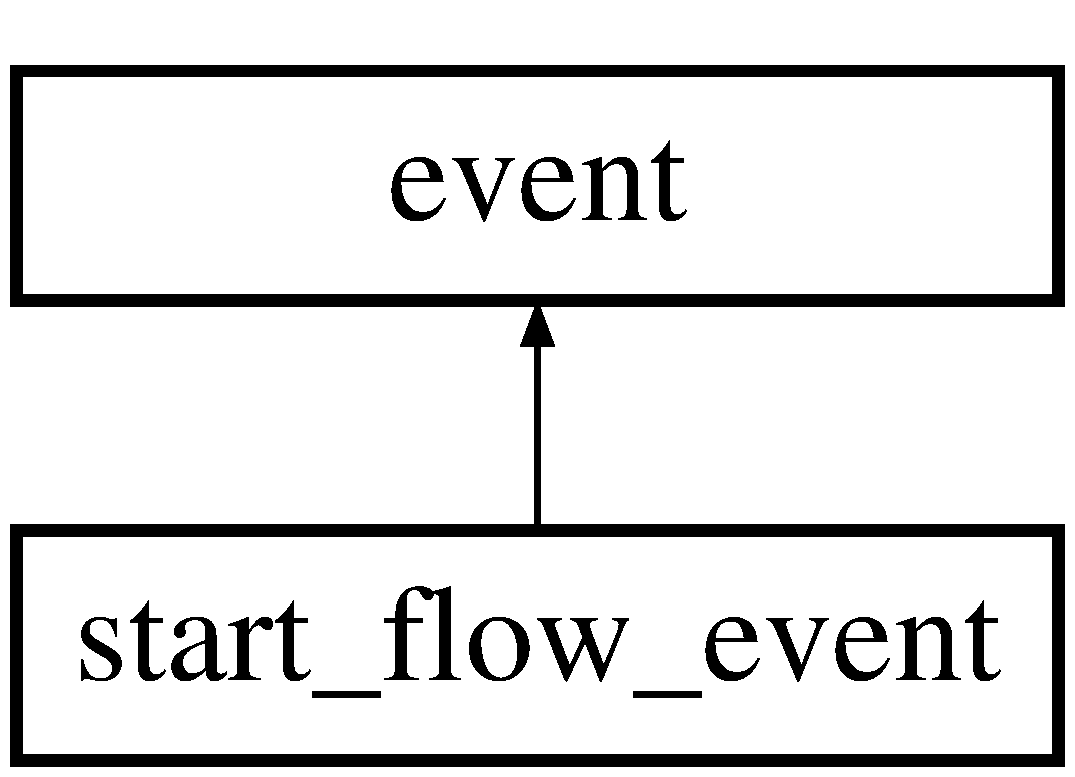
\includegraphics[height=2.000000cm]{classstart__flow__event}
\end{center}
\end{figure}
\subsection*{Public Member Functions}
\begin{DoxyCompactItemize}
\item 
\hypertarget{classstart__flow__event_a90655a3096c3f9112e95cc725582dcca}{\hyperlink{classstart__flow__event_a90655a3096c3f9112e95cc725582dcca}{start\-\_\-flow\-\_\-event} (double time, \hyperlink{classsimulation}{simulation} \&\hyperlink{classevent_a08c6d828bfb6f5539dcd1491e8ac77d2}{sim}, \hyperlink{classnetflow}{netflow} \&flow)}\label{classstart__flow__event_a90655a3096c3f9112e95cc725582dcca}

\begin{DoxyCompactList}\small\item\em Initializes this event's time to the given one, sets the event I\-D, and sets the flow that this \hyperlink{classstart__flow__event}{start\-\_\-flow\-\_\-event} is going to start. \end{DoxyCompactList}\item 
\hyperlink{classstart__flow__event_ad2892a0ae75b1438cd3bfa7839a21be1}{$\sim$start\-\_\-flow\-\_\-event} ()
\begin{DoxyCompactList}\small\item\em Destructor. \end{DoxyCompactList}\item 
\hypertarget{classstart__flow__event_a91f8f55565468bc294d89ccba846f759}{void \hyperlink{classstart__flow__event_a91f8f55565468bc294d89ccba846f759}{run\-Event} ()}\label{classstart__flow__event_a91f8f55565468bc294d89ccba846f759}

\begin{DoxyCompactList}\small\item\em Sends the first packet in this event's flow and queues a \hyperlink{classtimeout__event}{timeout\-\_\-event} internally and on the simulation event queue. \end{DoxyCompactList}\item 
void \hyperlink{classstart__flow__event_a75f4d4c3599f5ebc7813caccf07cde54}{print\-Helper} (ostream \&os)
\begin{DoxyCompactList}\small\item\em Print helper function. \end{DoxyCompactList}\end{DoxyCompactItemize}
\subsection*{Additional Inherited Members}


\subsection{Detailed Description}
Event that runs when a flow is about to start. 

Sends the first packet and has the flow register a timeout event internally and queue it up in the simulation's event queue. 

\subsection{Constructor \& Destructor Documentation}
\hypertarget{classstart__flow__event_ad2892a0ae75b1438cd3bfa7839a21be1}{\index{start\-\_\-flow\-\_\-event@{start\-\_\-flow\-\_\-event}!$\sim$start\-\_\-flow\-\_\-event@{$\sim$start\-\_\-flow\-\_\-event}}
\index{$\sim$start\-\_\-flow\-\_\-event@{$\sim$start\-\_\-flow\-\_\-event}!start_flow_event@{start\-\_\-flow\-\_\-event}}
\subsubsection[{$\sim$start\-\_\-flow\-\_\-event}]{\setlength{\rightskip}{0pt plus 5cm}start\-\_\-flow\-\_\-event\-::$\sim$start\-\_\-flow\-\_\-event (
\begin{DoxyParamCaption}
{}
\end{DoxyParamCaption}
)}}\label{classstart__flow__event_ad2892a0ae75b1438cd3bfa7839a21be1}


Destructor. 



\subsection{Member Function Documentation}
\hypertarget{classstart__flow__event_a75f4d4c3599f5ebc7813caccf07cde54}{\index{start\-\_\-flow\-\_\-event@{start\-\_\-flow\-\_\-event}!print\-Helper@{print\-Helper}}
\index{print\-Helper@{print\-Helper}!start_flow_event@{start\-\_\-flow\-\_\-event}}
\subsubsection[{print\-Helper}]{\setlength{\rightskip}{0pt plus 5cm}void start\-\_\-flow\-\_\-event\-::print\-Helper (
\begin{DoxyParamCaption}
\item[{ostream \&}]{os}
\end{DoxyParamCaption}
)\hspace{0.3cm}{\ttfamily [virtual]}}}\label{classstart__flow__event_a75f4d4c3599f5ebc7813caccf07cde54}


Print helper function. 


\begin{DoxyParams}{Parameters}
{\em os} & The output stream to which to write event information. \\
\hline
\end{DoxyParams}


Reimplemented from \hyperlink{classevent_a14ef1b59ef1f5a8311c7cac315c271df}{event}.



The documentation for this class was generated from the following files\-:\begin{DoxyCompactItemize}
\item 
src/\hyperlink{events_8h}{events.\-h}\item 
src/events.\-cpp\end{DoxyCompactItemize}

\hypertarget{classtimeout__event}{\section{timeout\-\_\-event Class Reference}
\label{classtimeout__event}\index{timeout\-\_\-event@{timeout\-\_\-event}}
}


Event that sets the window size to one then sends a packet.  




{\ttfamily \#include $<$events.\-h$>$}

Inheritance diagram for timeout\-\_\-event\-:\begin{figure}[H]
\begin{center}
\leavevmode
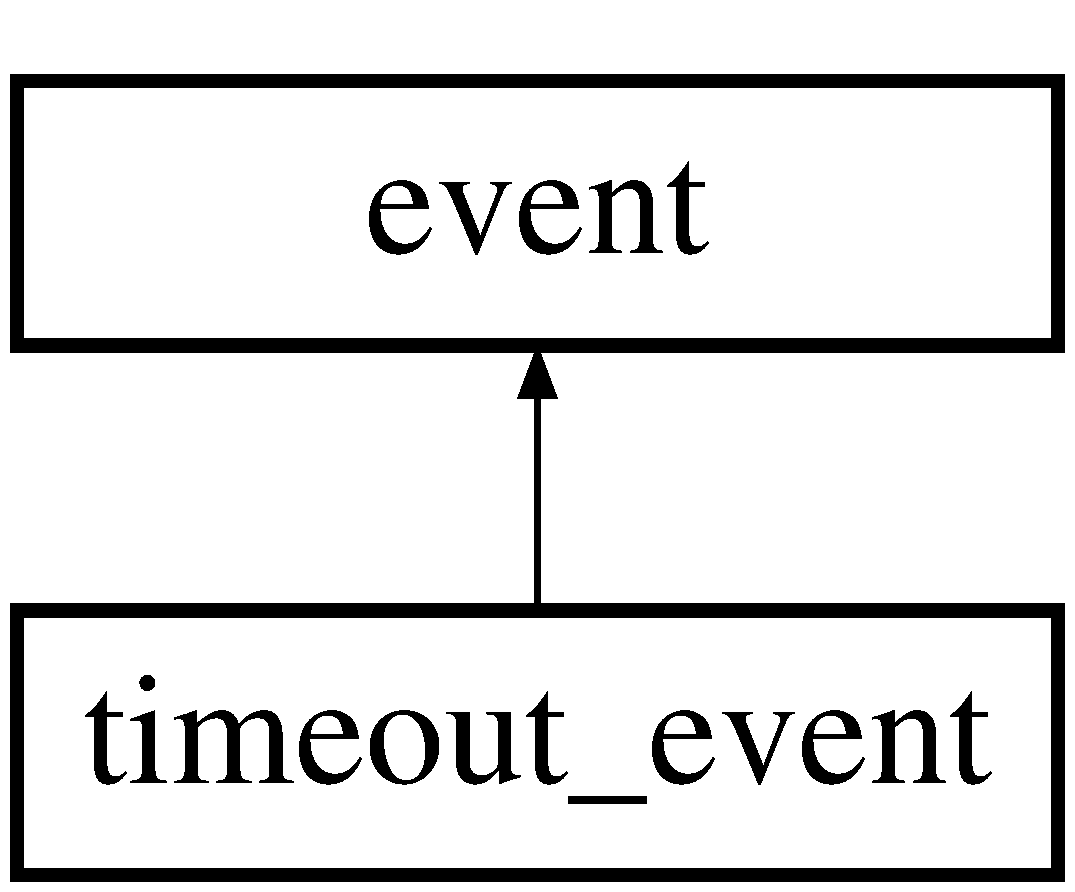
\includegraphics[height=2.000000cm]{classtimeout__event}
\end{center}
\end{figure}
\subsection*{Public Member Functions}
\begin{DoxyCompactItemize}
\item 
\hyperlink{classtimeout__event_a9388710e5b8e267f3221861ffb1444b4}{timeout\-\_\-event} ()
\begin{DoxyCompactList}\small\item\em Default constructor, sets everything to dummy or N\-U\-L\-L. \end{DoxyCompactList}\item 
\hyperlink{classtimeout__event_afbffa2152738dca0620e10cc60d16cb7}{timeout\-\_\-event} (double time, \hyperlink{classsimulation}{simulation} \&\hyperlink{classevent_a08c6d828bfb6f5539dcd1491e8ac77d2}{sim}, \hyperlink{classnetflow}{netflow} \&flow, int seqnum)
\begin{DoxyCompactList}\small\item\em Initializes this event's time to the given one, sets the event I\-D, and sets the flow to which this \hyperlink{classtimeout__event}{timeout\-\_\-event} belongs. \end{DoxyCompactList}\item 
\hyperlink{classtimeout__event_a8c3be1ba5886d9cb34bc7a257cc2d12c}{$\sim$timeout\-\_\-event} ()
\begin{DoxyCompactList}\small\item\em Destructor. \end{DoxyCompactList}\item 
void \hyperlink{classtimeout__event_abacd620618ef70149548ca014fa7fd57}{run\-Event} ()
\begin{DoxyCompactList}\small\item\em Registers a timeout with the flow, which means it changes its window size and linear growth threshold internally. \end{DoxyCompactList}\item 
void \hyperlink{classtimeout__event_a0c9c73de650b271dccfc6a7d3dedd3ec}{print\-Helper} (ostream \&os)
\begin{DoxyCompactList}\small\item\em Print helper function. \end{DoxyCompactList}\end{DoxyCompactItemize}
\subsection*{Additional Inherited Members}


\subsection{Detailed Description}
Event that sets the window size to one then sends a packet. 

This event queues another \hyperlink{classtimeout__event}{timeout\-\_\-event}; timeout\-\_\-events are chained so that the flow will keep trying to send packets in the face of timeouts indefinitely. \begin{DoxyRefDesc}{Deprecated}
\item[\hyperlink{deprecated__deprecated000001}{Deprecated}]because timeouts aren't currently being used \end{DoxyRefDesc}


\subsection{Constructor \& Destructor Documentation}
\hypertarget{classtimeout__event_a9388710e5b8e267f3221861ffb1444b4}{\index{timeout\-\_\-event@{timeout\-\_\-event}!timeout\-\_\-event@{timeout\-\_\-event}}
\index{timeout\-\_\-event@{timeout\-\_\-event}!timeout_event@{timeout\-\_\-event}}
\subsubsection[{timeout\-\_\-event}]{\setlength{\rightskip}{0pt plus 5cm}timeout\-\_\-event\-::timeout\-\_\-event (
\begin{DoxyParamCaption}
{}
\end{DoxyParamCaption}
)}}\label{classtimeout__event_a9388710e5b8e267f3221861ffb1444b4}


Default constructor, sets everything to dummy or N\-U\-L\-L. 

\hypertarget{classtimeout__event_afbffa2152738dca0620e10cc60d16cb7}{\index{timeout\-\_\-event@{timeout\-\_\-event}!timeout\-\_\-event@{timeout\-\_\-event}}
\index{timeout\-\_\-event@{timeout\-\_\-event}!timeout_event@{timeout\-\_\-event}}
\subsubsection[{timeout\-\_\-event}]{\setlength{\rightskip}{0pt plus 5cm}timeout\-\_\-event\-::timeout\-\_\-event (
\begin{DoxyParamCaption}
\item[{double}]{time, }
\item[{{\bf simulation} \&}]{sim, }
\item[{{\bf netflow} \&}]{flow, }
\item[{int}]{seqnum}
\end{DoxyParamCaption}
)}}\label{classtimeout__event_afbffa2152738dca0620e10cc60d16cb7}


Initializes this event's time to the given one, sets the event I\-D, and sets the flow to which this \hyperlink{classtimeout__event}{timeout\-\_\-event} belongs. 


\begin{DoxyParams}{Parameters}
{\em time} & \\
\hline
{\em sim} & \\
\hline
{\em flow} & \\
\hline
{\em seqnum} & \\
\hline
\end{DoxyParams}
\hypertarget{classtimeout__event_a8c3be1ba5886d9cb34bc7a257cc2d12c}{\index{timeout\-\_\-event@{timeout\-\_\-event}!$\sim$timeout\-\_\-event@{$\sim$timeout\-\_\-event}}
\index{$\sim$timeout\-\_\-event@{$\sim$timeout\-\_\-event}!timeout_event@{timeout\-\_\-event}}
\subsubsection[{$\sim$timeout\-\_\-event}]{\setlength{\rightskip}{0pt plus 5cm}timeout\-\_\-event\-::$\sim$timeout\-\_\-event (
\begin{DoxyParamCaption}
{}
\end{DoxyParamCaption}
)}}\label{classtimeout__event_a8c3be1ba5886d9cb34bc7a257cc2d12c}


Destructor. 



\subsection{Member Function Documentation}
\hypertarget{classtimeout__event_a0c9c73de650b271dccfc6a7d3dedd3ec}{\index{timeout\-\_\-event@{timeout\-\_\-event}!print\-Helper@{print\-Helper}}
\index{print\-Helper@{print\-Helper}!timeout_event@{timeout\-\_\-event}}
\subsubsection[{print\-Helper}]{\setlength{\rightskip}{0pt plus 5cm}void timeout\-\_\-event\-::print\-Helper (
\begin{DoxyParamCaption}
\item[{ostream \&}]{os}
\end{DoxyParamCaption}
)\hspace{0.3cm}{\ttfamily [virtual]}}}\label{classtimeout__event_a0c9c73de650b271dccfc6a7d3dedd3ec}


Print helper function. 


\begin{DoxyParams}{Parameters}
{\em os} & The output stream to which to write event information. \\
\hline
\end{DoxyParams}


Reimplemented from \hyperlink{classevent_a14ef1b59ef1f5a8311c7cac315c271df}{event}.

\hypertarget{classtimeout__event_abacd620618ef70149548ca014fa7fd57}{\index{timeout\-\_\-event@{timeout\-\_\-event}!run\-Event@{run\-Event}}
\index{run\-Event@{run\-Event}!timeout_event@{timeout\-\_\-event}}
\subsubsection[{run\-Event}]{\setlength{\rightskip}{0pt plus 5cm}void timeout\-\_\-event\-::run\-Event (
\begin{DoxyParamCaption}
{}
\end{DoxyParamCaption}
)\hspace{0.3cm}{\ttfamily [virtual]}}}\label{classtimeout__event_abacd620618ef70149548ca014fa7fd57}


Registers a timeout with the flow, which means it changes its window size and linear growth threshold internally. 

This function also chains (queues another) \hyperlink{classtimeout__event}{timeout\-\_\-event} and sends a packet by queueing a new \hyperlink{classsend__packet__event}{send\-\_\-packet\-\_\-event}. 

Reimplemented from \hyperlink{classevent_a74b7b9e3b4dd30fb42a2612968def7ef}{event}.



The documentation for this class was generated from the following files\-:\begin{DoxyCompactItemize}
\item 
src/\hyperlink{events_8h}{events.\-h}\item 
src/events.\-cpp\end{DoxyCompactItemize}

\hypertarget{classupdate__window__event}{\section{update\-\_\-window\-\_\-event Class Reference}
\label{classupdate__window__event}\index{update\-\_\-window\-\_\-event@{update\-\_\-window\-\_\-event}}
}


Event that triggers update of a given flow's window size.  




{\ttfamily \#include $<$events.\-h$>$}

Inheritance diagram for update\-\_\-window\-\_\-event\-:\begin{figure}[H]
\begin{center}
\leavevmode
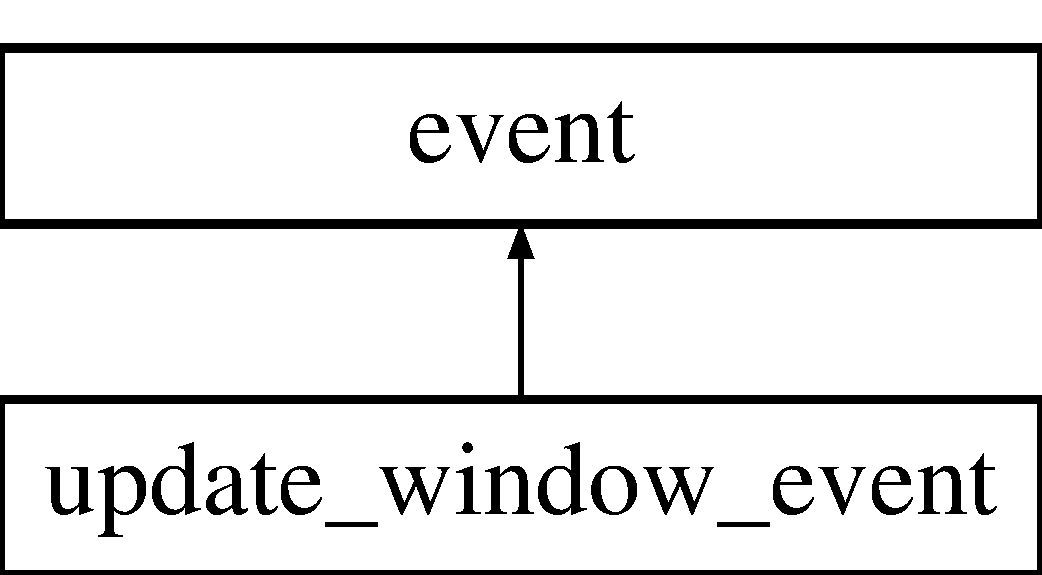
\includegraphics[height=2.000000cm]{classupdate__window__event}
\end{center}
\end{figure}
\subsection*{Public Member Functions}
\begin{DoxyCompactItemize}
\item 
\hyperlink{classupdate__window__event_ae243ddae54a04702f79154e0737f18c1}{update\-\_\-window\-\_\-event} (double time, \hyperlink{classsimulation}{simulation} \&\hyperlink{classevent_a08c6d828bfb6f5539dcd1491e8ac77d2}{sim}, \hyperlink{classnetflow}{netflow} \&flow)
\begin{DoxyCompactList}\small\item\em Constructor. \end{DoxyCompactList}\item 
\hyperlink{classupdate__window__event_a6210f1bc9245acd5f9038bc985528258}{$\sim$update\-\_\-window\-\_\-event} ()
\begin{DoxyCompactList}\small\item\em Destructor. \end{DoxyCompactList}\item 
void \hyperlink{classupdate__window__event_a41d9c1b343cd0ddceef94de6bc4abb68}{run\-Event} ()
\begin{DoxyCompactList}\small\item\em Updates window size based on F\-A\-S\-T specifications. \end{DoxyCompactList}\item 
void \hyperlink{classupdate__window__event_ae533c05504abbf5dd9285a375c44e307}{print\-Helper} (ostream \&os)
\begin{DoxyCompactList}\small\item\em Print helper function. \end{DoxyCompactList}\end{DoxyCompactItemize}
\subsection*{Additional Inherited Members}


\subsection{Detailed Description}
Event that triggers update of a given flow's window size. 

Only to be used for F\-A\-S\-T T\-C\-P. 

\subsection{Constructor \& Destructor Documentation}
\hypertarget{classupdate__window__event_ae243ddae54a04702f79154e0737f18c1}{\index{update\-\_\-window\-\_\-event@{update\-\_\-window\-\_\-event}!update\-\_\-window\-\_\-event@{update\-\_\-window\-\_\-event}}
\index{update\-\_\-window\-\_\-event@{update\-\_\-window\-\_\-event}!update_window_event@{update\-\_\-window\-\_\-event}}
\subsubsection[{update\-\_\-window\-\_\-event}]{\setlength{\rightskip}{0pt plus 5cm}update\-\_\-window\-\_\-event\-::update\-\_\-window\-\_\-event (
\begin{DoxyParamCaption}
\item[{double}]{time, }
\item[{{\bf simulation} \&}]{sim, }
\item[{{\bf netflow} \&}]{flow}
\end{DoxyParamCaption}
)}}\label{classupdate__window__event_ae243ddae54a04702f79154e0737f18c1}


Constructor. 


\begin{DoxyParams}{Parameters}
{\em time} & \\
\hline
{\em sim} & \\
\hline
{\em flow} & \\
\hline
\end{DoxyParams}
\hypertarget{classupdate__window__event_a6210f1bc9245acd5f9038bc985528258}{\index{update\-\_\-window\-\_\-event@{update\-\_\-window\-\_\-event}!$\sim$update\-\_\-window\-\_\-event@{$\sim$update\-\_\-window\-\_\-event}}
\index{$\sim$update\-\_\-window\-\_\-event@{$\sim$update\-\_\-window\-\_\-event}!update_window_event@{update\-\_\-window\-\_\-event}}
\subsubsection[{$\sim$update\-\_\-window\-\_\-event}]{\setlength{\rightskip}{0pt plus 5cm}update\-\_\-window\-\_\-event\-::$\sim$update\-\_\-window\-\_\-event (
\begin{DoxyParamCaption}
{}
\end{DoxyParamCaption}
)}}\label{classupdate__window__event_a6210f1bc9245acd5f9038bc985528258}


Destructor. 



\subsection{Member Function Documentation}
\hypertarget{classupdate__window__event_ae533c05504abbf5dd9285a375c44e307}{\index{update\-\_\-window\-\_\-event@{update\-\_\-window\-\_\-event}!print\-Helper@{print\-Helper}}
\index{print\-Helper@{print\-Helper}!update_window_event@{update\-\_\-window\-\_\-event}}
\subsubsection[{print\-Helper}]{\setlength{\rightskip}{0pt plus 5cm}void update\-\_\-window\-\_\-event\-::print\-Helper (
\begin{DoxyParamCaption}
\item[{ostream \&}]{os}
\end{DoxyParamCaption}
)\hspace{0.3cm}{\ttfamily [virtual]}}}\label{classupdate__window__event_ae533c05504abbf5dd9285a375c44e307}


Print helper function. 


\begin{DoxyParams}{Parameters}
{\em os} & The output stream to which to write event information. \\
\hline
\end{DoxyParams}


Reimplemented from \hyperlink{classevent_a14ef1b59ef1f5a8311c7cac315c271df}{event}.

\hypertarget{classupdate__window__event_a41d9c1b343cd0ddceef94de6bc4abb68}{\index{update\-\_\-window\-\_\-event@{update\-\_\-window\-\_\-event}!run\-Event@{run\-Event}}
\index{run\-Event@{run\-Event}!update_window_event@{update\-\_\-window\-\_\-event}}
\subsubsection[{run\-Event}]{\setlength{\rightskip}{0pt plus 5cm}void update\-\_\-window\-\_\-event\-::run\-Event (
\begin{DoxyParamCaption}
{}
\end{DoxyParamCaption}
)\hspace{0.3cm}{\ttfamily [virtual]}}}\label{classupdate__window__event_a41d9c1b343cd0ddceef94de6bc4abb68}


Updates window size based on F\-A\-S\-T specifications. 



Reimplemented from \hyperlink{classevent_a74b7b9e3b4dd30fb42a2612968def7ef}{event}.



The documentation for this class was generated from the following files\-:\begin{DoxyCompactItemize}
\item 
src/\hyperlink{events_8h}{events.\-h}\item 
src/events.\-cpp\end{DoxyCompactItemize}

\chapter{File Documentation}
\hypertarget{plotNetSimData_8py}{\section{plot/plot\-Net\-Sim\-Data.py File Reference}
\label{plotNetSimData_8py}\index{plot/plot\-Net\-Sim\-Data.\-py@{plot/plot\-Net\-Sim\-Data.\-py}}
}


In Network Simulation project for Caltech C\-S 143, the following metrics are measured and then graphed as a time trace and overall average.  


\subsection*{Functions}
\begin{DoxyCompactItemize}
\item 
def {\bfseries plot\-Net\-Sim\-Data.\-load\-All\-Data}
\item 
def {\bfseries plot\-Net\-Sim\-Data.\-make\-Leg\-Dict}
\item 
def {\bfseries plot\-Net\-Sim\-Data.\-plot\-Link\-Data}
\item 
def {\bfseries plot\-Net\-Sim\-Data.\-plot\-Flow\-Data}
\item 
def {\bfseries plot\-Net\-Sim\-Data.\-plot\-All}
\end{DoxyCompactItemize}
\subsection*{Variables}
\begin{DoxyCompactItemize}
\item 
\hypertarget{namespaceplotNetSimData_aae1bbe552e8fe69410ab16b082f4614e}{list {\bfseries plot\-Net\-Sim\-Data.\-filename} = sys.\-argv\mbox{[}1\mbox{]}}\label{namespaceplotNetSimData_aae1bbe552e8fe69410ab16b082f4614e}

\end{DoxyCompactItemize}


\subsection{Detailed Description}
In Network Simulation project for Caltech C\-S 143, the following metrics are measured and then graphed as a time trace and overall average. For each link\-: link rate (Mbps), buffer occupancy (is this one per link?), packet loss. For each flow\-: flow rate, window size, packet delay. The simulator records data into a .json file, from which data is extracted and graphed.

For each subplot in each window (Link Metric, Flow Metric), the viewer can choose which data set to view by clicking on the associated line 'symbol' in the subplot's legend. This feature is most helpful when comparing link flow rates, since the data sets all overlap and become hard to make sense of. 
\hypertarget{driver_8cpp}{\section{src/driver.cpp File Reference}
\label{driver_8cpp}\index{src/driver.\-cpp@{src/driver.\-cpp}}
}


This file reads a network description from a J\-S\-O\-N file then starts a simulation of the network.  


{\ttfamily \#include $<$iostream$>$}\\*
{\ttfamily \#include $<$string$>$}\\*
{\ttfamily \#include $<$cstdlib$>$}\\*
{\ttfamily \#include $<$string.\-h$>$}\\*
{\ttfamily \#include \char`\"{}simulation.\-h\char`\"{}}\\*
\subsection*{Functions}
\begin{DoxyCompactItemize}
\item 
void \hyperlink{driver_8cpp_ab978b4842ecd248235f5a14142cd9666}{print\-\_\-usage\-\_\-statement} (char $\ast$progname)
\begin{DoxyCompactList}\small\item\em Prints a usage statement to stderr. \end{DoxyCompactList}\item 
char $\ast$ \hyperlink{driver_8cpp_a1ce59744bad236bde5b7e5fcebb20cae}{process\-\_\-console\-\_\-args} (int argc, char $\ast$$\ast$argv)
\begin{DoxyCompactList}\small\item\em Processes console arguments, returning the input filename and setting flags like the debug one. \end{DoxyCompactList}\item 
\hypertarget{driver_8cpp_a3c04138a5bfe5d72780bb7e82a18e627}{int \hyperlink{driver_8cpp_a3c04138a5bfe5d72780bb7e82a18e627}{main} (int argc, char $\ast$$\ast$argv)}\label{driver_8cpp_a3c04138a5bfe5d72780bb7e82a18e627}

\begin{DoxyCompactList}\small\item\em Reads a J\-S\-O\-N file from disk, populates in-\/memory collections of hosts, routers, links, and flows, starts a simulation, then logs data. \end{DoxyCompactList}\end{DoxyCompactItemize}
\subsection*{Variables}
\begin{DoxyCompactItemize}
\item 
bool \hyperlink{driver_8cpp_a398527b3e9e358c345c5047b16871957}{debug} = false
\begin{DoxyCompactList}\small\item\em If true lots of debugging output is shown. \end{DoxyCompactList}\item 
\hypertarget{driver_8cpp_a7766f78695ce29e0b42fa8966015711b}{bool \hyperlink{driver_8cpp_a7766f78695ce29e0b42fa8966015711b}{detail} = false}\label{driver_8cpp_a7766f78695ce29e0b42fa8966015711b}

\begin{DoxyCompactList}\small\item\em If true even more debugging output is shown and the output pauses between events for analysis. \end{DoxyCompactList}\item 
ostream \& \hyperlink{driver_8cpp_a8e1c5eaa16af1f8c320bd11588d11fba}{debug\-\_\-os} = cout
\begin{DoxyCompactList}\small\item\em Output stream to which to write debugging statements. \end{DoxyCompactList}\end{DoxyCompactItemize}


\subsection{Detailed Description}
This file reads a network description from a J\-S\-O\-N file then starts a simulation of the network. It logs data as the simulation progresses then dumps it to to disk so scripts can generate graphs. 

\subsection{Function Documentation}
\hypertarget{driver_8cpp_ab978b4842ecd248235f5a14142cd9666}{\index{driver.\-cpp@{driver.\-cpp}!print\-\_\-usage\-\_\-statement@{print\-\_\-usage\-\_\-statement}}
\index{print\-\_\-usage\-\_\-statement@{print\-\_\-usage\-\_\-statement}!driver.cpp@{driver.\-cpp}}
\subsubsection[{print\-\_\-usage\-\_\-statement}]{\setlength{\rightskip}{0pt plus 5cm}void print\-\_\-usage\-\_\-statement (
\begin{DoxyParamCaption}
\item[{char $\ast$}]{progname}
\end{DoxyParamCaption}
)}}\label{driver_8cpp_ab978b4842ecd248235f5a14142cd9666}


Prints a usage statement to stderr. 


\begin{DoxyParams}{Parameters}
{\em progname} & name of this program. \\
\hline
\end{DoxyParams}
\hypertarget{driver_8cpp_a1ce59744bad236bde5b7e5fcebb20cae}{\index{driver.\-cpp@{driver.\-cpp}!process\-\_\-console\-\_\-args@{process\-\_\-console\-\_\-args}}
\index{process\-\_\-console\-\_\-args@{process\-\_\-console\-\_\-args}!driver.cpp@{driver.\-cpp}}
\subsubsection[{process\-\_\-console\-\_\-args}]{\setlength{\rightskip}{0pt plus 5cm}char $\ast$ process\-\_\-console\-\_\-args (
\begin{DoxyParamCaption}
\item[{int}]{argc, }
\item[{char $\ast$$\ast$}]{argv}
\end{DoxyParamCaption}
)}}\label{driver_8cpp_a1ce59744bad236bde5b7e5fcebb20cae}


Processes console arguments, returning the input filename and setting flags like the debug one. 


\begin{DoxyParams}{Parameters}
{\em argc} & number of console arguments \\
\hline
{\em argv} & console arguments \\
\hline
\end{DoxyParams}
\begin{DoxyReturn}{Returns}
the input filename 
\end{DoxyReturn}
\begin{DoxyPostcond}{Postcondition}
sets the debug flag 
\end{DoxyPostcond}
\begin{DoxyWarning}{Warning}
exits from this process after printing a usage statement if the console arguments don't conform to the usage statement 
\end{DoxyWarning}


\subsection{Variable Documentation}
\hypertarget{driver_8cpp_a398527b3e9e358c345c5047b16871957}{\index{driver.\-cpp@{driver.\-cpp}!debug@{debug}}
\index{debug@{debug}!driver.cpp@{driver.\-cpp}}
\subsubsection[{debug}]{\setlength{\rightskip}{0pt plus 5cm}bool debug = false}}\label{driver_8cpp_a398527b3e9e358c345c5047b16871957}


If true lots of debugging output is shown. 

\hypertarget{driver_8cpp_a8e1c5eaa16af1f8c320bd11588d11fba}{\index{driver.\-cpp@{driver.\-cpp}!debug\-\_\-os@{debug\-\_\-os}}
\index{debug\-\_\-os@{debug\-\_\-os}!driver.cpp@{driver.\-cpp}}
\subsubsection[{debug\-\_\-os}]{\setlength{\rightskip}{0pt plus 5cm}ostream\& debug\-\_\-os = cout}}\label{driver_8cpp_a8e1c5eaa16af1f8c320bd11588d11fba}


Output stream to which to write debugging statements. 

Might be customized to be a file output stream, stderr, or something else. 
\hypertarget{events_8h}{\section{src/events.h File Reference}
\label{events_8h}\index{src/events.\-h@{src/events.\-h}}
}


Contains the declarations of all the event classes used in this simulation.  


{\ttfamily \#include $<$iostream$>$}\\*
{\ttfamily \#include \char`\"{}util.\-h\char`\"{}}\\*
{\ttfamily \#include \char`\"{}network.\-h\char`\"{}}\\*
\subsection*{Classes}
\begin{DoxyCompactItemize}
\item 
class \hyperlink{classevent}{event}
\begin{DoxyCompactList}\small\item\em Base class for events in our event-\/driven network simulation. \end{DoxyCompactList}\item 
class \hyperlink{classreceive__packet__event}{receive\-\_\-packet\-\_\-event}
\begin{DoxyCompactList}\small\item\em Event that represents the arrival of a packet at either an intermediate node (router) or a final destination (host). \end{DoxyCompactList}\item 
class \hyperlink{classrouter__discovery__event}{router\-\_\-discovery\-\_\-event}
\begin{DoxyCompactList}\small\item\em Event that triggers a given router's routing-\/table-\/population algorithm. \end{DoxyCompactList}\item 
class \hyperlink{classupdate__window__event}{update\-\_\-window\-\_\-event}
\begin{DoxyCompactList}\small\item\em Event that triggers update of a given flow's window size. \end{DoxyCompactList}\item 
class \hyperlink{classsend__packet__event}{send\-\_\-packet\-\_\-event}
\begin{DoxyCompactList}\small\item\em Sends a packet from a given departure node and down a given link whether it's an A\-C\-K, F\-L\-O\-W, or R\-O\-U\-T\-I\-N\-G packet. \end{DoxyCompactList}\item 
class \hyperlink{classstart__flow__event}{start\-\_\-flow\-\_\-event}
\begin{DoxyCompactList}\small\item\em Event that runs when a flow is about to start. \end{DoxyCompactList}\item 
class \hyperlink{classtimeout__event}{timeout\-\_\-event}
\begin{DoxyCompactList}\small\item\em Event that sets the window size to one then sends a packet. \end{DoxyCompactList}\item 
class \hyperlink{classack__event}{ack\-\_\-event}
\begin{DoxyCompactList}\small\item\em This event should be queued when a destination host wants to send an A\-C\-K (not just duplicate A\-C\-Ks--any A\-C\-K\-S). \end{DoxyCompactList}\end{DoxyCompactItemize}
\subsection*{Functions}
\begin{DoxyCompactItemize}
\item 
ostream \& \hyperlink{events_8h_aecd9498c45f5bcd05faf5837347c35be}{operator$<$$<$} (ostream \&os, \hyperlink{classevent}{event} \&e)
\begin{DoxyCompactList}\small\item\em Output operator override for printing contents of the given event to an output stream. \end{DoxyCompactList}\end{DoxyCompactItemize}
\subsection*{Variables}
\begin{DoxyCompactItemize}
\item 
bool \hyperlink{events_8h_a398527b3e9e358c345c5047b16871957}{debug}
\begin{DoxyCompactList}\small\item\em If true lots of debugging output is shown. \end{DoxyCompactList}\item 
\hypertarget{events_8h_a7766f78695ce29e0b42fa8966015711b}{bool \hyperlink{events_8h_a7766f78695ce29e0b42fa8966015711b}{detail}}\label{events_8h_a7766f78695ce29e0b42fa8966015711b}

\begin{DoxyCompactList}\small\item\em If true even more debugging output is shown and the output pauses between events for analysis. \end{DoxyCompactList}\item 
ostream \& \hyperlink{events_8h_a8e1c5eaa16af1f8c320bd11588d11fba}{debug\-\_\-os}
\begin{DoxyCompactList}\small\item\em Output stream to which to write debugging statements. \end{DoxyCompactList}\end{DoxyCompactItemize}


\subsection{Detailed Description}
Contains the declarations of all the event classes used in this simulation. Objects of these events are put onto an event queu in a global simulation object. 

\subsection{Function Documentation}
\hypertarget{events_8h_aecd9498c45f5bcd05faf5837347c35be}{\index{events.\-h@{events.\-h}!operator$<$$<$@{operator$<$$<$}}
\index{operator$<$$<$@{operator$<$$<$}!events.h@{events.\-h}}
\subsubsection[{operator$<$$<$}]{\setlength{\rightskip}{0pt plus 5cm}ostream\& operator$<$$<$ (
\begin{DoxyParamCaption}
\item[{ostream \&}]{os, }
\item[{{\bf event} \&}]{e}
\end{DoxyParamCaption}
)\hspace{0.3cm}{\ttfamily [inline]}}}\label{events_8h_aecd9498c45f5bcd05faf5837347c35be}


Output operator override for printing contents of the given event to an output stream. 

Uses the print\-Helper function, which is virtual because derived classes will want to modify or enhance printing behavior. 
\begin{DoxyParams}{Parameters}
{\em os} & The output stream to which to write. \\
\hline
{\em device} & The {\ttfamily event} object to write. \\
\hline
\end{DoxyParams}
\begin{DoxyReturn}{Returns}
The same output stream for operator chaining. 
\end{DoxyReturn}


\subsection{Variable Documentation}
\hypertarget{events_8h_a398527b3e9e358c345c5047b16871957}{\index{events.\-h@{events.\-h}!debug@{debug}}
\index{debug@{debug}!events.h@{events.\-h}}
\subsubsection[{debug}]{\setlength{\rightskip}{0pt plus 5cm}bool debug}}\label{events_8h_a398527b3e9e358c345c5047b16871957}


If true lots of debugging output is shown. 

\hypertarget{events_8h_a8e1c5eaa16af1f8c320bd11588d11fba}{\index{events.\-h@{events.\-h}!debug\-\_\-os@{debug\-\_\-os}}
\index{debug\-\_\-os@{debug\-\_\-os}!events.h@{events.\-h}}
\subsubsection[{debug\-\_\-os}]{\setlength{\rightskip}{0pt plus 5cm}ostream\& debug\-\_\-os}}\label{events_8h_a8e1c5eaa16af1f8c320bd11588d11fba}


Output stream to which to write debugging statements. 

Might be customized to be a file output stream, stderr, or something else. 
\hypertarget{network_8h}{\section{src/network.h File Reference}
\label{network_8h}\index{src/network.\-h@{src/network.\-h}}
}


Contains the declarations of all the network device classes as well as the packet class.  


{\ttfamily \#include $<$iostream$>$}\\*
{\ttfamily \#include $<$cassert$>$}\\*
{\ttfamily \#include $<$string$>$}\\*
{\ttfamily \#include $<$vector$>$}\\*
{\ttfamily \#include $<$map$>$}\\*
{\ttfamily \#include $<$queue$>$}\\*
{\ttfamily \#include $<$cmath$>$}\\*
{\ttfamily \#include $<$limits$>$}\\*
{\ttfamily \#include $<$set$>$}\\*
{\ttfamily \#include \char`\"{}util.\-h\char`\"{}}\\*
\subsection*{Classes}
\begin{DoxyCompactItemize}
\item 
class \hyperlink{classnetelement}{netelement}
\begin{DoxyCompactList}\small\item\em Superclass of all network elements including routers, hosts, links, packets, flows. \end{DoxyCompactList}\item 
class \hyperlink{classnetnode}{netnode}
\begin{DoxyCompactList}\small\item\em Represents a node, which is either a node or a host, in a simple network. \end{DoxyCompactList}\item 
class \hyperlink{classnethost}{nethost}
\begin{DoxyCompactList}\small\item\em Represents a host. \end{DoxyCompactList}\item 
class \hyperlink{classnetrouter}{netrouter}
\begin{DoxyCompactList}\small\item\em Represents a router in a simple network. \end{DoxyCompactList}\item 
class \hyperlink{classnetflow}{netflow}
\begin{DoxyCompactList}\small\item\em Represents a flow in a simple network. \end{DoxyCompactList}\item 
class \hyperlink{classnetlink}{netlink}
\begin{DoxyCompactList}\small\item\em Represents a half-\/duplex link. \end{DoxyCompactList}\item 
class \hyperlink{classpacket}{packet}
\begin{DoxyCompactList}\small\item\em Describes a packet in the simulated network, which can be one of the types in the enumerated type {\ttfamily packet\-Type}. \end{DoxyCompactList}\end{DoxyCompactItemize}
\subsection*{Functions}
\begin{DoxyCompactItemize}
\item 
ostream \& \hyperlink{network_8h_a255e0a140c7fdb2984c3efb7c13ea63a}{operator$<$$<$} (ostream \&os, const \hyperlink{classnetelement}{netelement} \&device)
\begin{DoxyCompactList}\small\item\em Output operator override for printing contents of the given netelement to an output stream. \end{DoxyCompactList}\end{DoxyCompactItemize}
\subsection*{Variables}
\begin{DoxyCompactItemize}
\item 
bool \hyperlink{network_8h_a398527b3e9e358c345c5047b16871957}{debug}
\begin{DoxyCompactList}\small\item\em If true lots of debugging output is shown. \end{DoxyCompactList}\item 
\hypertarget{network_8h_a7766f78695ce29e0b42fa8966015711b}{bool \hyperlink{network_8h_a7766f78695ce29e0b42fa8966015711b}{detail}}\label{network_8h_a7766f78695ce29e0b42fa8966015711b}

\begin{DoxyCompactList}\small\item\em If true even more debugging output is shown and the output pauses between events for analysis. \end{DoxyCompactList}\item 
ostream \& \hyperlink{network_8h_a8e1c5eaa16af1f8c320bd11588d11fba}{debug\-\_\-os}
\begin{DoxyCompactList}\small\item\em Output stream to which to write debugging statements. \end{DoxyCompactList}\end{DoxyCompactItemize}


\subsection{Detailed Description}
Contains the declarations of all the network device classes as well as the packet class. 

\subsection{Function Documentation}
\hypertarget{network_8h_a255e0a140c7fdb2984c3efb7c13ea63a}{\index{network.\-h@{network.\-h}!operator$<$$<$@{operator$<$$<$}}
\index{operator$<$$<$@{operator$<$$<$}!network.h@{network.\-h}}
\subsubsection[{operator$<$$<$}]{\setlength{\rightskip}{0pt plus 5cm}ostream\& operator$<$$<$ (
\begin{DoxyParamCaption}
\item[{ostream \&}]{os, }
\item[{const {\bf netelement} \&}]{device}
\end{DoxyParamCaption}
)\hspace{0.3cm}{\ttfamily [inline]}}}\label{network_8h_a255e0a140c7fdb2984c3efb7c13ea63a}


Output operator override for printing contents of the given netelement to an output stream. 

Uses the print\-Helper function, which is virtual because derived classes will want to modify or enhance printing behavior. 
\begin{DoxyParams}{Parameters}
{\em os} & The output stream to which to write. \\
\hline
{\em device} & The {\ttfamily netdevice} object to write. \\
\hline
\end{DoxyParams}
\begin{DoxyReturn}{Returns}
The same output stream for operator chaining. 
\end{DoxyReturn}


\subsection{Variable Documentation}
\hypertarget{network_8h_a398527b3e9e358c345c5047b16871957}{\index{network.\-h@{network.\-h}!debug@{debug}}
\index{debug@{debug}!network.h@{network.\-h}}
\subsubsection[{debug}]{\setlength{\rightskip}{0pt plus 5cm}bool debug}}\label{network_8h_a398527b3e9e358c345c5047b16871957}


If true lots of debugging output is shown. 

\hypertarget{network_8h_a8e1c5eaa16af1f8c320bd11588d11fba}{\index{network.\-h@{network.\-h}!debug\-\_\-os@{debug\-\_\-os}}
\index{debug\-\_\-os@{debug\-\_\-os}!network.h@{network.\-h}}
\subsubsection[{debug\-\_\-os}]{\setlength{\rightskip}{0pt plus 5cm}ostream\& debug\-\_\-os}}\label{network_8h_a8e1c5eaa16af1f8c320bd11588d11fba}


Output stream to which to write debugging statements. 

Might be customized to be a file output stream, stderr, or something else. 
\hypertarget{simulation_8h}{\section{src/simulation.h File Reference}
\label{simulation_8h}\index{src/simulation.\-h@{src/simulation.\-h}}
}


Contains the declaration of the simulation class.  


{\ttfamily \#include $<$iostream$>$}\\*
{\ttfamily \#include $<$map$>$}\\*
{\ttfamily \#include $<$string$>$}\\*
{\ttfamily \#include $<$sstream$>$}\\*
{\ttfamily \#include $<$cassert$>$}\\*
{\ttfamily \#include $<$fstream$>$}\\*
{\ttfamily \#include $<$cstdlib$>$}\\*
{\ttfamily \#include $<$vector$>$}\\*
{\ttfamily \#include $<$queue$>$}\\*
{\ttfamily \#include \char`\"{}rapidjson/document.\-h\char`\"{}}\\*
{\ttfamily \#include \char`\"{}rapidjson/prettywriter.\-h\char`\"{}}\\*
{\ttfamily \#include \char`\"{}json.\-hpp\char`\"{}}\\*
{\ttfamily \#include \char`\"{}events.\-h\char`\"{}}\\*
\subsection*{Classes}
\begin{DoxyCompactItemize}
\item 
class \hyperlink{classsimulation}{simulation}
\begin{DoxyCompactList}\small\item\em Represents the simulation. \end{DoxyCompactList}\end{DoxyCompactItemize}
\subsection*{Variables}
\begin{DoxyCompactItemize}
\item 
bool \hyperlink{simulation_8h_a398527b3e9e358c345c5047b16871957}{debug}
\begin{DoxyCompactList}\small\item\em If true lots of debugging output is shown. \end{DoxyCompactList}\item 
\hypertarget{simulation_8h_a7766f78695ce29e0b42fa8966015711b}{bool \hyperlink{simulation_8h_a7766f78695ce29e0b42fa8966015711b}{detail}}\label{simulation_8h_a7766f78695ce29e0b42fa8966015711b}

\begin{DoxyCompactList}\small\item\em If true even more debugging output is shown and the output pauses between events for analysis. \end{DoxyCompactList}\item 
ostream \& \hyperlink{simulation_8h_a8e1c5eaa16af1f8c320bd11588d11fba}{debug\-\_\-os}
\begin{DoxyCompactList}\small\item\em Output stream to which to write debugging statements. \end{DoxyCompactList}\end{DoxyCompactItemize}


\subsection{Detailed Description}
Contains the declaration of the simulation class. 

\subsection{Variable Documentation}
\hypertarget{simulation_8h_a398527b3e9e358c345c5047b16871957}{\index{simulation.\-h@{simulation.\-h}!debug@{debug}}
\index{debug@{debug}!simulation.h@{simulation.\-h}}
\subsubsection[{debug}]{\setlength{\rightskip}{0pt plus 5cm}bool debug}}\label{simulation_8h_a398527b3e9e358c345c5047b16871957}


If true lots of debugging output is shown. 

\hypertarget{simulation_8h_a8e1c5eaa16af1f8c320bd11588d11fba}{\index{simulation.\-h@{simulation.\-h}!debug\-\_\-os@{debug\-\_\-os}}
\index{debug\-\_\-os@{debug\-\_\-os}!simulation.h@{simulation.\-h}}
\subsubsection[{debug\-\_\-os}]{\setlength{\rightskip}{0pt plus 5cm}ostream\& debug\-\_\-os}}\label{simulation_8h_a8e1c5eaa16af1f8c320bd11588d11fba}


Output stream to which to write debugging statements. 

Might be customized to be a file output stream, stderr, or something else. 
\hypertarget{util_8h}{\section{src/util.h File Reference}
\label{util_8h}\index{src/util.\-h@{src/util.\-h}}
}


Contains some constants used in the simulation.  


\subsection*{Enumerations}
\begin{DoxyCompactItemize}
\item 
enum \hyperlink{util_8h_ad875bcb78f9bd8625c5e454cafdc8de7}{packet\-\_\-type} \{ {\bfseries F\-L\-O\-W}, 
{\bfseries A\-C\-K}, 
{\bfseries R\-O\-U\-T\-I\-N\-G}
 \}
\begin{DoxyCompactList}\small\item\em Types of packets in this simulation. \end{DoxyCompactList}\end{DoxyCompactItemize}
\subsection*{Variables}
\begin{DoxyCompactItemize}
\item 
\hypertarget{util_8h_ae9a63afe84927184ec4534e7c97e6ab9}{const int {\bfseries B\-Y\-T\-E\-S\-\_\-\-P\-E\-R\-\_\-\-K\-B} = 1 $<$$<$ 10}\label{util_8h_ae9a63afe84927184ec4534e7c97e6ab9}

\item 
const int \hyperlink{util_8h_a45ef21db68c5dce33f9aec6625c531f8}{K\-B\-\_\-\-P\-E\-R\-\_\-\-M\-B} = 1 $<$$<$ 10
\begin{DoxyCompactList}\small\item\em Conversion factor between kilobytes and megabytes. \end{DoxyCompactList}\item 
const int \hyperlink{util_8h_a2840a0c52ba094c789a284869e2c417a}{B\-I\-T\-S\-\_\-\-P\-E\-R\-\_\-\-B\-Y\-T\-E} = 1 $<$$<$ 3
\begin{DoxyCompactList}\small\item\em Conversion factor between bits and bytes. \end{DoxyCompactList}\item 
const int \hyperlink{util_8h_a140e08844115e442f89b9b526a58b0bd}{B\-Y\-T\-E\-S\-\_\-\-P\-E\-R\-\_\-\-M\-E\-G\-A\-B\-I\-T}
\begin{DoxyCompactList}\small\item\em Input rate is in mbps, so this is used to convert to bytes per sec. \end{DoxyCompactList}\item 
const int \hyperlink{util_8h_a45898693f5ddd3cabb39bb3ac5c16793}{M\-S\-\_\-\-P\-E\-R\-\_\-\-S\-E\-C} = 1000
\begin{DoxyCompactList}\small\item\em Milliseconds per second. \end{DoxyCompactList}\item 
const int \hyperlink{util_8h_a97638ffeb0b5bf246854b456686cd3c3}{S\-E\-Q\-N\-U\-M\-\_\-\-F\-O\-R\-\_\-\-N\-O\-N\-F\-L\-O\-W\-S} = -\/1
\begin{DoxyCompactList}\small\item\em A sentinel used for the sequence numbers of routing packets. \end{DoxyCompactList}\item 
\hypertarget{util_8h_a5adf921c40bdaa0582410019d965be40}{const int \hyperlink{util_8h_a5adf921c40bdaa0582410019d965be40}{R\-A\-T\-E\-\_\-\-I\-N\-T\-E\-R\-V\-A\-L} = 1000}\label{util_8h_a5adf921c40bdaa0582410019d965be40}

\begin{DoxyCompactList}\small\item\em Time interval in ms over which to compute flow rate. \end{DoxyCompactList}\item 
const int \hyperlink{util_8h_ae49e8e5338b41e720159a8ba378f27de}{U\-P\-P\-E\-R\-\_\-\-T\-I\-M\-E\-\_\-\-R\-O\-U\-T\-I\-N\-G\-\_\-\-L\-I\-M\-I\-T} = 400000
\begin{DoxyCompactList}\small\item\em Send routing packets until this time (in milliseconds) is reached. \end{DoxyCompactList}\item 
const int \hyperlink{util_8h_ae87dc2b3c270e2ec909b938654f9655d}{P\-R\-I\-N\-T\-\_\-\-P\-A\-C\-K\-E\-T\-\_\-\-I\-N\-F\-O\-\_\-\-M\-I\-L\-E\-S\-T\-O\-N\-E} = 5000
\begin{DoxyCompactList}\small\item\em Print information about packets every (this many) packets. \end{DoxyCompactList}\item 
const int \hyperlink{util_8h_a40feb99f64f03ba8095b82df9a4cbbb4}{L\-O\-G\-\_\-\-F\-R\-E\-Q\-U\-E\-N\-C\-Y} = 10
\begin{DoxyCompactList}\small\item\em Log every (this many) events. \end{DoxyCompactList}\item 
const double \hyperlink{util_8h_ad52560045a9084dd30b72a194f358168}{G\-A\-M\-M\-A} = 0.\-5
\begin{DoxyCompactList}\small\item\em Fairness parameter for F\-A\-S\-T T\-C\-P. \end{DoxyCompactList}\item 
const double \hyperlink{util_8h_a29874299171f0e96c480b139d19adef4}{A\-L\-P\-H\-A} = 20
\begin{DoxyCompactList}\small\item\em Fairness parameter for F\-A\-S\-T T\-C\-P. \end{DoxyCompactList}\end{DoxyCompactItemize}


\subsection{Detailed Description}
Contains some constants used in the simulation. 

\subsection{Enumeration Type Documentation}
\hypertarget{util_8h_ad875bcb78f9bd8625c5e454cafdc8de7}{\index{util.\-h@{util.\-h}!packet\-\_\-type@{packet\-\_\-type}}
\index{packet\-\_\-type@{packet\-\_\-type}!util.h@{util.\-h}}
\subsubsection[{packet\-\_\-type}]{\setlength{\rightskip}{0pt plus 5cm}enum {\bf packet\-\_\-type}}}\label{util_8h_ad875bcb78f9bd8625c5e454cafdc8de7}


Types of packets in this simulation. 



\subsection{Variable Documentation}
\hypertarget{util_8h_a29874299171f0e96c480b139d19adef4}{\index{util.\-h@{util.\-h}!A\-L\-P\-H\-A@{A\-L\-P\-H\-A}}
\index{A\-L\-P\-H\-A@{A\-L\-P\-H\-A}!util.h@{util.\-h}}
\subsubsection[{A\-L\-P\-H\-A}]{\setlength{\rightskip}{0pt plus 5cm}const double A\-L\-P\-H\-A = 20}}\label{util_8h_a29874299171f0e96c480b139d19adef4}


Fairness parameter for F\-A\-S\-T T\-C\-P. 

Currently each flow uses the same values. \hypertarget{util_8h_a2840a0c52ba094c789a284869e2c417a}{\index{util.\-h@{util.\-h}!B\-I\-T\-S\-\_\-\-P\-E\-R\-\_\-\-B\-Y\-T\-E@{B\-I\-T\-S\-\_\-\-P\-E\-R\-\_\-\-B\-Y\-T\-E}}
\index{B\-I\-T\-S\-\_\-\-P\-E\-R\-\_\-\-B\-Y\-T\-E@{B\-I\-T\-S\-\_\-\-P\-E\-R\-\_\-\-B\-Y\-T\-E}!util.h@{util.\-h}}
\subsubsection[{B\-I\-T\-S\-\_\-\-P\-E\-R\-\_\-\-B\-Y\-T\-E}]{\setlength{\rightskip}{0pt plus 5cm}const int B\-I\-T\-S\-\_\-\-P\-E\-R\-\_\-\-B\-Y\-T\-E = 1 $<$$<$ 3}}\label{util_8h_a2840a0c52ba094c789a284869e2c417a}


Conversion factor between bits and bytes. 

\hypertarget{util_8h_a140e08844115e442f89b9b526a58b0bd}{\index{util.\-h@{util.\-h}!B\-Y\-T\-E\-S\-\_\-\-P\-E\-R\-\_\-\-M\-E\-G\-A\-B\-I\-T@{B\-Y\-T\-E\-S\-\_\-\-P\-E\-R\-\_\-\-M\-E\-G\-A\-B\-I\-T}}
\index{B\-Y\-T\-E\-S\-\_\-\-P\-E\-R\-\_\-\-M\-E\-G\-A\-B\-I\-T@{B\-Y\-T\-E\-S\-\_\-\-P\-E\-R\-\_\-\-M\-E\-G\-A\-B\-I\-T}!util.h@{util.\-h}}
\subsubsection[{B\-Y\-T\-E\-S\-\_\-\-P\-E\-R\-\_\-\-M\-E\-G\-A\-B\-I\-T}]{\setlength{\rightskip}{0pt plus 5cm}const int B\-Y\-T\-E\-S\-\_\-\-P\-E\-R\-\_\-\-M\-E\-G\-A\-B\-I\-T}}\label{util_8h_a140e08844115e442f89b9b526a58b0bd}
{\bfseries Initial value\-:}
\begin{DoxyCode}
=
        BYTES\_PER\_KB * \hyperlink{util_8h_a45ef21db68c5dce33f9aec6625c531f8}{KB\_PER\_MB} / \hyperlink{util_8h_a2840a0c52ba094c789a284869e2c417a}{BITS\_PER\_BYTE}
\end{DoxyCode}


Input rate is in mbps, so this is used to convert to bytes per sec. 

\hypertarget{util_8h_ad52560045a9084dd30b72a194f358168}{\index{util.\-h@{util.\-h}!G\-A\-M\-M\-A@{G\-A\-M\-M\-A}}
\index{G\-A\-M\-M\-A@{G\-A\-M\-M\-A}!util.h@{util.\-h}}
\subsubsection[{G\-A\-M\-M\-A}]{\setlength{\rightskip}{0pt plus 5cm}const double G\-A\-M\-M\-A = 0.\-5}}\label{util_8h_ad52560045a9084dd30b72a194f358168}


Fairness parameter for F\-A\-S\-T T\-C\-P. 

Currently each flow uses the same values. \hypertarget{util_8h_a45ef21db68c5dce33f9aec6625c531f8}{\index{util.\-h@{util.\-h}!K\-B\-\_\-\-P\-E\-R\-\_\-\-M\-B@{K\-B\-\_\-\-P\-E\-R\-\_\-\-M\-B}}
\index{K\-B\-\_\-\-P\-E\-R\-\_\-\-M\-B@{K\-B\-\_\-\-P\-E\-R\-\_\-\-M\-B}!util.h@{util.\-h}}
\subsubsection[{K\-B\-\_\-\-P\-E\-R\-\_\-\-M\-B}]{\setlength{\rightskip}{0pt plus 5cm}const int K\-B\-\_\-\-P\-E\-R\-\_\-\-M\-B = 1 $<$$<$ 10}}\label{util_8h_a45ef21db68c5dce33f9aec6625c531f8}


Conversion factor between kilobytes and megabytes. 

\hypertarget{util_8h_a40feb99f64f03ba8095b82df9a4cbbb4}{\index{util.\-h@{util.\-h}!L\-O\-G\-\_\-\-F\-R\-E\-Q\-U\-E\-N\-C\-Y@{L\-O\-G\-\_\-\-F\-R\-E\-Q\-U\-E\-N\-C\-Y}}
\index{L\-O\-G\-\_\-\-F\-R\-E\-Q\-U\-E\-N\-C\-Y@{L\-O\-G\-\_\-\-F\-R\-E\-Q\-U\-E\-N\-C\-Y}!util.h@{util.\-h}}
\subsubsection[{L\-O\-G\-\_\-\-F\-R\-E\-Q\-U\-E\-N\-C\-Y}]{\setlength{\rightskip}{0pt plus 5cm}const int L\-O\-G\-\_\-\-F\-R\-E\-Q\-U\-E\-N\-C\-Y = 10}}\label{util_8h_a40feb99f64f03ba8095b82df9a4cbbb4}


Log every (this many) events. 

\hypertarget{util_8h_a45898693f5ddd3cabb39bb3ac5c16793}{\index{util.\-h@{util.\-h}!M\-S\-\_\-\-P\-E\-R\-\_\-\-S\-E\-C@{M\-S\-\_\-\-P\-E\-R\-\_\-\-S\-E\-C}}
\index{M\-S\-\_\-\-P\-E\-R\-\_\-\-S\-E\-C@{M\-S\-\_\-\-P\-E\-R\-\_\-\-S\-E\-C}!util.h@{util.\-h}}
\subsubsection[{M\-S\-\_\-\-P\-E\-R\-\_\-\-S\-E\-C}]{\setlength{\rightskip}{0pt plus 5cm}const int M\-S\-\_\-\-P\-E\-R\-\_\-\-S\-E\-C = 1000}}\label{util_8h_a45898693f5ddd3cabb39bb3ac5c16793}


Milliseconds per second. 

\hypertarget{util_8h_ae87dc2b3c270e2ec909b938654f9655d}{\index{util.\-h@{util.\-h}!P\-R\-I\-N\-T\-\_\-\-P\-A\-C\-K\-E\-T\-\_\-\-I\-N\-F\-O\-\_\-\-M\-I\-L\-E\-S\-T\-O\-N\-E@{P\-R\-I\-N\-T\-\_\-\-P\-A\-C\-K\-E\-T\-\_\-\-I\-N\-F\-O\-\_\-\-M\-I\-L\-E\-S\-T\-O\-N\-E}}
\index{P\-R\-I\-N\-T\-\_\-\-P\-A\-C\-K\-E\-T\-\_\-\-I\-N\-F\-O\-\_\-\-M\-I\-L\-E\-S\-T\-O\-N\-E@{P\-R\-I\-N\-T\-\_\-\-P\-A\-C\-K\-E\-T\-\_\-\-I\-N\-F\-O\-\_\-\-M\-I\-L\-E\-S\-T\-O\-N\-E}!util.h@{util.\-h}}
\subsubsection[{P\-R\-I\-N\-T\-\_\-\-P\-A\-C\-K\-E\-T\-\_\-\-I\-N\-F\-O\-\_\-\-M\-I\-L\-E\-S\-T\-O\-N\-E}]{\setlength{\rightskip}{0pt plus 5cm}const int P\-R\-I\-N\-T\-\_\-\-P\-A\-C\-K\-E\-T\-\_\-\-I\-N\-F\-O\-\_\-\-M\-I\-L\-E\-S\-T\-O\-N\-E = 5000}}\label{util_8h_ae87dc2b3c270e2ec909b938654f9655d}


Print information about packets every (this many) packets. 

\hypertarget{util_8h_a97638ffeb0b5bf246854b456686cd3c3}{\index{util.\-h@{util.\-h}!S\-E\-Q\-N\-U\-M\-\_\-\-F\-O\-R\-\_\-\-N\-O\-N\-F\-L\-O\-W\-S@{S\-E\-Q\-N\-U\-M\-\_\-\-F\-O\-R\-\_\-\-N\-O\-N\-F\-L\-O\-W\-S}}
\index{S\-E\-Q\-N\-U\-M\-\_\-\-F\-O\-R\-\_\-\-N\-O\-N\-F\-L\-O\-W\-S@{S\-E\-Q\-N\-U\-M\-\_\-\-F\-O\-R\-\_\-\-N\-O\-N\-F\-L\-O\-W\-S}!util.h@{util.\-h}}
\subsubsection[{S\-E\-Q\-N\-U\-M\-\_\-\-F\-O\-R\-\_\-\-N\-O\-N\-F\-L\-O\-W\-S}]{\setlength{\rightskip}{0pt plus 5cm}const int S\-E\-Q\-N\-U\-M\-\_\-\-F\-O\-R\-\_\-\-N\-O\-N\-F\-L\-O\-W\-S = -\/1}}\label{util_8h_a97638ffeb0b5bf246854b456686cd3c3}


A sentinel used for the sequence numbers of routing packets. 

\hypertarget{util_8h_ae49e8e5338b41e720159a8ba378f27de}{\index{util.\-h@{util.\-h}!U\-P\-P\-E\-R\-\_\-\-T\-I\-M\-E\-\_\-\-R\-O\-U\-T\-I\-N\-G\-\_\-\-L\-I\-M\-I\-T@{U\-P\-P\-E\-R\-\_\-\-T\-I\-M\-E\-\_\-\-R\-O\-U\-T\-I\-N\-G\-\_\-\-L\-I\-M\-I\-T}}
\index{U\-P\-P\-E\-R\-\_\-\-T\-I\-M\-E\-\_\-\-R\-O\-U\-T\-I\-N\-G\-\_\-\-L\-I\-M\-I\-T@{U\-P\-P\-E\-R\-\_\-\-T\-I\-M\-E\-\_\-\-R\-O\-U\-T\-I\-N\-G\-\_\-\-L\-I\-M\-I\-T}!util.h@{util.\-h}}
\subsubsection[{U\-P\-P\-E\-R\-\_\-\-T\-I\-M\-E\-\_\-\-R\-O\-U\-T\-I\-N\-G\-\_\-\-L\-I\-M\-I\-T}]{\setlength{\rightskip}{0pt plus 5cm}const int U\-P\-P\-E\-R\-\_\-\-T\-I\-M\-E\-\_\-\-R\-O\-U\-T\-I\-N\-G\-\_\-\-L\-I\-M\-I\-T = 400000}}\label{util_8h_ae49e8e5338b41e720159a8ba378f27de}


Send routing packets until this time (in milliseconds) is reached. 


%--- End generated contents ---

% Index
\newpage
\phantomsection
\addcontentsline{toc}{chapter}{Index}
\printindex

\end{document}
